%=======================================================================
% Multi-Agent Research Orchestrator --- MASTER HINGLISH NOTES (150 Pages)
% Story-Based | Line-by-Line Code | 60+ Interview Q&A | System Design
%=======================================================================
\documentclass[11pt, a4paper]{article}

% -- Packages ----------------------------------------------------------
\usepackage[utf8]{inputenc}
\usepackage[T1]{fontenc}
\usepackage{lmodern}
\usepackage[margin=0.8in]{geometry}
\usepackage[table,xcdraw]{xcolor}
\usepackage{listings}
\usepackage{tcolorbox}
\usepackage{enumitem}
\usepackage{hyperref}
\usepackage{fancyhdr}
\usepackage{titlesec}
\usepackage{graphicx}
\usepackage{booktabs}
\usepackage{longtable}
\usepackage{amsmath}
\usepackage{amssymb}
\usepackage{tikz}
\usetikzlibrary{shapes.geometric, arrows.meta, positioning, calc, decorations.pathmorphing, fit}
\usepackage{multicol}
\usepackage{fancyvrb}
\usepackage{mdframed}
\usepackage{fontawesome5}
\usepackage{tabularx}
\usepackage{float}
\usepackage{caption}
\usepackage{parskip}

\tcbuselibrary{listings, skins, breakable}

% -- Colors ------------------------------------------------------------
\definecolor{bg}{HTML}{1a1a2e}
\definecolor{codebg}{HTML}{0d1117}
\definecolor{codeframe}{HTML}{30363d}
\definecolor{keyword}{HTML}{ff79c6}
\definecolor{string}{HTML}{f1fa8c}
\definecolor{comment}{HTML}{6272a4}
\definecolor{function}{HTML}{50fa7b}
\definecolor{accentpurple}{HTML}{bd93f9}
\definecolor{accentblue}{HTML}{8be9fd}
\definecolor{accentorange}{HTML}{ffb86c}
\definecolor{accentred}{HTML}{ff5555}
\definecolor{accentgreen}{HTML}{50fa7b}
\definecolor{notebg}{HTML}{fff8e1}
\definecolor{tipbg}{HTML}{e8f5e9}
\definecolor{warnbg}{HTML}{fff3e0}
\definecolor{importantbg}{HTML}{e3f2fd}
\definecolor{deepbg}{HTML}{f3e5f5}
\definecolor{storybg}{HTML}{fce4ec}

% -- Code Listing Styles -----------------------------------------------
\lstdefinestyle{pythonstyle}{
    language=Python,
    basicstyle=\small\ttfamily\color{white},
    backgroundcolor=\color{codebg},
    keywordstyle=\color{keyword}\bfseries,
    stringstyle=\color{string},
    commentstyle=\color{comment}\itshape,
    numberstyle=\tiny\color{comment},
    numbers=left,
    numbersep=8pt,
    frame=single,
    rulecolor=\color{codeframe},
    breaklines=true,
    breakatwhitespace=false,
    showstringspaces=false,
    tabsize=4,
    captionpos=b,
    morekeywords={self, True, False, None, as, with, yield, async, await},
    emph={ResearchState, ChatGroq, TavilyClient, StateGraph, END, Chroma,
          HuggingFaceEmbeddings, PyPDFLoader, RecursiveCharacterTextSplitter,
          TypedDict, Annotated, FastMCP, APIView, Response, ModelSerializer},
    emphstyle=\color{accentblue}\bfseries,
    emph={[2]researcher_node, analyst_node, fact_checker_node, writer_node,
          build_graph, should_continue, get_embeddings, get_vectorstore,
          ingest_documents, retrieve_context, store_research_session,
          research_topic, ingest_document, search_knowledge_base,
          run_single_agent_baseline, evaluate_outputs},
    emphstyle={[2]\color{accentgreen}},
    literate={->}{{\textcolor{accentorange}{$\rightarrow$}}}1
             {<-}{{\textcolor{accentorange}{$\leftarrow$}}}1,
}

\lstdefinestyle{envstyle}{
    basicstyle=\small\ttfamily\color{white},
    backgroundcolor=\color{codebg},
    frame=single,
    rulecolor=\color{codeframe},
    breaklines=true,
    numbers=left,
    numberstyle=\tiny\color{comment},
    numbersep=8pt,
    commentstyle=\color{comment}\itshape,
    morecomment=[l]{\#},
}

\lstdefinestyle{bashstyle}{
    basicstyle=\small\ttfamily\color{accentgreen},
    backgroundcolor=\color{codebg},
    frame=single,
    rulecolor=\color{codeframe},
    breaklines=true,
    numbers=none,
}

\lstdefinestyle{jsonstyle}{
    basicstyle=\small\ttfamily\color{white},
    backgroundcolor=\color{codebg},
    frame=single,
    rulecolor=\color{codeframe},
    breaklines=true,
    numbers=left,
    numberstyle=\tiny\color{comment},
    numbersep=8pt,
    keywordstyle=\color{accentorange}\bfseries,
    stringstyle=\color{string},
    commentstyle=\color{comment}\itshape,
}

% -- tcolorbox Styles --------------------------------------------------
\newtcolorbox{notebox}[1][]{
    colback=notebg, colframe=accentorange!70!black,
    fonttitle=\bfseries, title={\faIcon{lightbulb} ~Yaad Rakhne Ka Tip},
    rounded corners, breakable, #1
}
\newtcolorbox{conceptbox}[1][]{
    colback=importantbg, colframe=accentblue!70!black,
    fonttitle=\bfseries, title={\faIcon{brain} ~Concept Deep Dive},
    rounded corners, breakable, #1
}
\newtcolorbox{storybox}[1][]{
    colback=storybg, colframe=accentred!60!black,
    fonttitle=\bfseries, title={\faIcon{book-open} ~Kahani Se Samjho},
    rounded corners, breakable, #1
}
\newtcolorbox{warningbox}[1][]{
    colback=warnbg, colframe=accentorange!80!black,
    fonttitle=\bfseries, title={\faIcon{exclamation-triangle} ~Dhyan Do},
    rounded corners, breakable, #1
}
\newtcolorbox{interviewbox}[1][]{
    colback=deepbg, colframe=accentpurple!70!black,
    fonttitle=\bfseries, title={\faIcon{user-tie} ~Interview Question},
    rounded corners, breakable, #1
}
\newtcolorbox{codestorybox}[1][]{
    colback=tipbg, colframe=accentgreen!70!black,
    fonttitle=\bfseries, title={\faIcon{code} ~Code Samjho Line-by-Line},
    rounded corners, breakable, #1
}
\newtcolorbox{mathbox}[1][]{
    colback=importantbg, colframe=accentblue!60!black,
    fonttitle=\bfseries, title={\faIcon{square-root-alt} ~Maths Behind the Scene},
    rounded corners, breakable, #1
}
\newtcolorbox{memorybox}[1][]{
    colback=notebg, colframe=accentorange!60!black,
    fonttitle=\bfseries, title={\faIcon{memory} ~Memory Trick},
    rounded corners, breakable, #1
}
\newtcolorbox{designbox}[1][]{
    colback=tipbg, colframe=accentgreen!80!black,
    fonttitle=\bfseries, title={\faIcon{cogs} ~System Design Deep Dive},
    rounded corners, breakable, #1
}

% -- Page Style --------------------------------------------------------
\pagestyle{fancy}
\fancyhf{}
\fancyhead[L]{\textcolor{accentpurple}{\small\textbf{Multi-Agent Research Orchestrator}}}
\fancyhead[R]{\textcolor{comment}{\small Master Hinglish Notes (150 Pages)}}
\fancyfoot[C]{\textcolor{accentblue}{\thepage}}
\renewcommand{\headrulewidth}{0.4pt}
\renewcommand{\headrule}{\hbox to\headwidth{\color{accentpurple}\leaders\hrule height \headrulewidth\hfill}}

% -- Section Formatting ------------------------------------------------
\titleformat{\section}{\LARGE\bfseries\color{accentpurple}}{
    \colorbox{accentpurple!15}{\makebox[2em]{\thesection}}}{0.5em}{}[
    \vspace{-0.5em}\color{accentpurple}\rule{\textwidth}{2pt}]

\titleformat{\subsection}{\Large\bfseries\color{accentblue}}{
    \thesubsection}{0.5em}{}[\vspace{-0.3em}\color{accentblue!40}\rule{0.7\textwidth}{0.5pt}]

\titleformat{\subsubsection}{\large\bfseries\color{accentorange}}{
    \thesubsubsection}{0.5em}{}

% -- Hyperref Setup ----------------------------------------------------
\hypersetup{
    colorlinks=true,
    linkcolor=accentpurple,
    urlcolor=accentblue,
    citecolor=accentgreen,
    bookmarks=true,
    bookmarksopen=true,
}

% -- Document Start ----------------------------------------------------
\begin{document}

% ======================================================================
% TITLE PAGE
% ======================================================================
\begin{titlepage}
\begin{center}
\vspace*{0.8cm}

\begin{tikzpicture}
  \node[circle, draw=accentpurple, line width=3pt, minimum size=3cm,
        fill=accentpurple!10] (center) {
    \Huge\color{accentpurple}\faIcon{microscope}
  };
  \foreach \angle/\icon/\col in {
    45/\faIcon{search}/accentblue,
    135/\faIcon{chart-bar}/accentgreen,
    225/\faIcon{check-circle}/accentorange,
    315/\faIcon{pen-fancy}/accentred%
  }{
    \node[circle, draw=\col, line width=2pt, minimum size=1.8cm,
          fill=\col!10] at (\angle:3.5cm) {\Large\color{\col}\icon};
    \draw[-{Stealth[length=3mm]}, \col, line width=1.5pt]
          (center.\angle) -- (\angle:2.5cm);
  }
\end{tikzpicture}

\vspace{1.2cm}
{\Huge\bfseries\color{accentpurple} Multi-Agent Research Orchestrator}\\[0.5cm]
{\LARGE\color{accentblue} The Complete Master Notes}\\[0.3cm]
{\large\color{comment} Story-Based Hinglish Deep Dive --- 150 Pages}\\[0.3cm]
{\large\color{comment} Line-by-Line Code $|$ RAG $|$ MCP $|$ Django $|$ Benchmark $|$ 60+ Interview Q\&A}

\vspace{1.2cm}

\begin{tikzpicture}
\node[draw=accentblue!50, rounded corners=10pt, fill=accentblue!5,
      text width=15cm, align=center, inner sep=14pt] {
    \color{accentblue}\large\textbf{Tech Stack at a Glance}\\[8pt]
    \begin{tabular}{ll}
    \color{keyword}\faIcon{brain} \textbf{LLM} & Groq (openai/gpt-oss-120b) \\
    \color{accentgreen}\faIcon{project-diagram} \textbf{Orchestration} & LangGraph StateGraph \\
    \color{accentorange}\faIcon{search} \textbf{Web Search} & Tavily API \\
    \color{accentblue}\faIcon{database} \textbf{Vector Store} & ChromaDB (Persistent) \\
    \color{string}\faIcon{robot} \textbf{Embeddings} & all-MiniLM-L6-v2 (Local, Free) \\
    \color{accentred}\faIcon{desktop} \textbf{UI} & Streamlit (3 Themes) \\
    \color{accentpurple}\faIcon{plug} \textbf{Protocol} & MCP via FastMCP \\
    \color{function}\faIcon{server} \textbf{REST Backend} & Django + DRF + Token Auth \\
    \color{accentorange}\faIcon{chart-line} \textbf{Benchmark} & Single vs Multi-Agent \\
    \color{function}\faIcon{python} \textbf{Language} & Python 3.12 \\
    \end{tabular}
};
\end{tikzpicture}

\vfill
{\color{comment}\today}
\end{center}
\end{titlepage}

% ======================================================================
% TABLE OF CONTENTS
% ======================================================================
\tableofcontents
\newpage

% ######################################################################
% HOW TO READ THIS BOOK
% ######################################################################
\section*{Kaise Padhein Yeh Book (How to Read This Book)}
\addcontentsline{toc}{section}{Kaise Padhein Yeh Book}

\begin{storybox}
Yeh book ek \textbf{research firm ki kahani} hai. Hum ek imaginary company banate hain jisme 4 expert employees hain --- \textbf{Khoji (Researcher)}, \textbf{Vishleshak (Analyst)}, \textbf{Satya-Parikshak (Fact Checker)} aur \textbf{Lekhak (Writer)}. Har chapter mein hum ek naya concept samjhenge, phir us concept ko code mein dekhenge, phir interview ke sawaal ka jawaab denge.

\textbf{Hinglish ka istemaal} isliye kiya hai kyunki jab aap apne dimaag mein concepts ko apni bhasha mein store karte ho, toh interview mein wapas nikalna easy hota hai. Technical terms English mein rakhe hain taaki interview mein wahi exact words bol sako.

\textbf{Reading Flow:}
\begin{enumerate}[label=\textcolor{accentpurple}{\arabic*.}]
\item Part I (Sections 1--3): Sirf kahani padho --- 30 minute mein poori project samajh aayegi.
\item Part II (Sections 4--8): Concepts deep dive --- har concept ka ``kyun'' samjho.
\item Part III (Sections 9--21): Code line-by-line --- har file ka har line.
\item Part IV (Sections 22--26): System design aur edge cases.
\item Part V (Sections 27--29): Interview Q\&A --- last minute revision.
\end{enumerate}
\end{storybox}

% ######################################################################
% PART I --- THE STORY
% ######################################################################
\section{Part I: The Story --- Ek Research Firm Ka Sapna}

\subsection{Kahani: Rahul Ka Placement Assignment}

\begin{storybox}
\textbf{Rahul} ek final-year CSE student hai (NIT Hamirpur, Dual Degree). Uske paas ek assignment hai: \textit{``Ek system banao jo kisi bhi topic par research karke report likhe.''}

Rahul pehle try karta hai:
\begin{verbatim}
prompt = "Research the impact of AI on healthcare and write a report."
report = llm.invoke(prompt)
\end{verbatim}

Ek hi LLM call se report milta hai. Par Rahul ko 3 problems dikhti hain:

\textbf{Problem 1 --- Hallucination (Jhooth):} LLM ne report mein facts bana diye jo exist nahi karte. Kyun? Kyunki LLM sirf next word predict karta hai --- wo ``sochta'' nahi hai ki kya sach hai. Wo apne training data se extrapolate karta hai.

\textbf{Problem 2 --- Ek Angle Wali Research:} Rahul ne poocha ``impact on healthcare''. LLM ne sirf ek generic summary diya. Usne \textbf{market size, technical challenges, regulations, startups} --- ye sab angles cover nahi kiye. Ek insaan researcher 10 sources padhta hai aur 5 angles se sochta hai. LLM ek hi baar mein ek angle deta hai.

\textbf{Problem 3 --- Verification Zero:} Report mein claims the par koi proof nahi tha. Kaise pata chalega ki ``AI can diagnose cancer 95\% accuracy'' ye sach hai? Koi source citation nahi tha.

Rahul ko realization hota hai: \textbf{Ek hi LLM call se research quality nahi aayegi.} Usse chahiye ek \textbf{pipeline} --- jahan kaam alag-alag experts ko milta hai, har expert apna kaam karta hai, aur koi expert galat ho toh system khud correct karta hai.
\end{storybox}

\subsection{Solution: 4 Agents, Ek Firm Ki Tarah}

\begin{conceptbox}
\textbf{Multi-Agent System ka concept:} Ek LLM ko multiple ``roles'' mein deploy karo --- har role ki apni responsibility, apna prompt, apni temperature setting. Ye agents ek sequence mein kaam karte hain aur ek dusre ke saath state share karte hain.

Humara pipeline:
\[
\text{Researcher} \longrightarrow \text{Analyst} \longrightarrow \text{Fact-Checker} \longrightarrow \text{Writer}
\]
Aur agar Fact-Checker ko galat claim milta hai:
\[
\text{Fact-Checker} \xrightarrow{\text{NEEDS\_REVISION}} \text{Researcher} \quad (\text{max 2 baar})
\]
\end{conceptbox}

\begin{storybox}
\textbf{Firm ka model:} Socho ek research firm jisme:

\begin{itemize}
\item \textbf{Khoji (Researcher):} Interviewer ki tarah --- topic ke 3 alag angles banata hai, internet par search karta hai (Tavily), aur company ke apne documents (PDFs) bhi padhta hai (ChromaDB RAG). Result: raw data.

\item \textbf{Vishleshak (Analyst):} Detective ki tarah --- raw data padhkar usme se \textbf{key themes} nikalta hai, \textbf{contradictions} flag karta hai (Source A kehti hai 2027, Source B kehta hai 2025), \textbf{consensus} batata hai, aur \textbf{gaps} dhundhta hai (kya information missing hai). Result: structured analysis.

\item \textbf{Satya-Parikshak (Fact Checker):} Auditor ki tarah --- analysis ka har claim raw sources se compare karta hai. Agar claim source se supported hai toh \texttt{PASSED}. Agar nahi, toh \texttt{NEEDS\_REVISION} + feedback notes. Result: verified or rejected analysis.

\item \textbf{Lekhak (Writer):} Senior technical writer ki tarah --- verified analysis ko ek publication-grade Markdown report mein convert karta hai, citations ke saath, aur session ko long-term memory (ChromaDB) mein save karta hai.
\end{itemize}
\end{storybox}

\subsection{Why 4 Agents and Not 1 Big Prompt?}

\begin{interviewbox}
\textbf{Q: ``4 alag agents kyun banaye? Ek hi LLM call mein sab kyun nahi karwaya?''}

\textbf{Answer (Hinglish):} 4 reasons:

\begin{enumerate}[label=\textcolor{accentpurple}{\arabic*.}]
\item \textbf{Separation of Concerns:} Agar ek prompt ko bolo ``search karo, analyze karo, fact-check karo, aur report likho'' toh wo har kaam mediocre karega. Kyunki ek prompt ka \textbf{focus} spread ho jata hai. Alag agents = har agent ka ek hi kaam = usme excellence.

\item \textbf{Alag-alag Temperature:} Har role ko alag ``creativity level'' chahiye:
  \begin{itemize}
  \item Researcher: \textbf{Temperature = 0.0} --- strict factual retrieval, koi creativity nahi.
  \item Analyst: \textbf{T = 0.2} --- structured logical deduction.
  \item Fact Checker: \textbf{T = 0.1} --- strict verification, zero assumptions.
  \item Writer: \textbf{T = 0.4} --- smooth professional prose.
  \end{itemize}
  Ek hi prompt mein multiple temperatures impossible hain.

\item \textbf{Confirmation Bias:} LLM apne hi likhe text ki galti khud nahi pakad sakta (same way hum apni typing mistakes khud nahi dekh paate). Independent Fact-Checker role \textbf{hallucinations catch} karta hai.

\item \textbf{Modularity:} Naye agents add karna easy hai --- e.g., ``Data Visualizer'' ya ``Code Sandbox'' --- bina existing graph ko toda.
\end{enumerate}
\end{interviewbox}

\subsection{Tech Stack Selection --- Har Choice Ka ``Kyun''}

\begin{designbox}
\textbf{Humne ye stack kyun chuna? Har choice ke peeche ek engineering trade-off hai:}

\begin{longtable}{p{3.2cm} p{4.5cm} p{5.5cm}}
\toprule
\textbf{Technology} & \textbf{Kyun chuna?} & \textbf{Kya alternative tha?} \\
\midrule
\textbf{Groq + GPT-OSS-120B} & LPU hardware se 250+ tok/s speed, free tier, multi-agent pipeline 6--8 sec mein. & OpenAI GPT-4o (30--45 sec, costly) \\
\textbf{LangGraph} & Explicit state machine: nodes, edges, conditional routing, cycles. Deterministic control. & CrewAI (black-box), AutoGen (chat loops, token burn) \\
\textbf{Tavily} & Search-optimized LLM API: clean content extraction, source URLs. & Google/Bing APIs (messy HTML parsing) \\
\textbf{ChromaDB} & Lightweight, persistent, local vector store, zero API cost, LangChain integration. & Pinecone (cloud, costly), FAISS (no persistence) \\
\textbf{all-MiniLM-L6-v2} & 80MB, 384-dim, CPU par fast, zero cost. & OpenAI embeddings (costly) \\
\textbf{Streamlit} & Python-native UI, rapid dev, real-time streaming. & React/Flask (slow dev) \\
\textbf{FastMCP} & MCP standard protocol --- Claude Desktop, Cursor connect karte hain. & Raw JSON-RPC (reinvent wheel) \\
\textbf{Django + DRF} & Production REST API: auth, ORM, admin, token auth. & FastAPI (lighter but less batteries) \\
\bottomrule
\end{longtable}
\end{designbox}

\begin{memorybox}
\textbf{Memory Trick --- ``S-L-A-C-K'':}
\textbf{S}earch (Tavily), \textbf{L}angGraph, \textbf{A}nalysis (agents), \textbf{C}hromaDB, \textbf{K}nowledge (RAG) --- ye 5 pillars project ke hain.
\end{memorybox}

% ######################################################################
% SECTION 2: THE STATE --- PIPELINE KA DIMAAG
% ######################################################################
\section{The State --- Pipeline Ka Dimaag (TypedDict + Reducers)}

\subsection{Concept: Agents Ek Dusre Se Direct Baat Nahi Karte}

\begin{storybox}
Socho 4 employees ek dusre ke saamne baith kar chillayenge toh chaos hoga. Iski jagah, ek \textbf{shared whiteboard (state)} hai. Har employee apna result whiteboard par likhta hai, aur agla employee whiteboard padhkar kaam karta hai.

LangGraph mein ye whiteboard ek \textbf{dictionary} hai --- \texttt{ResearchState}. Har agent function ek \textbf{partial update} return karta hai jo is dictionary mein merge hota hai.
\end{storybox}

\begin{conceptbox}
\textbf{TypedDict kya hai?} Python ka ek type-hinting tool jo batata hai ki dictionary mein \textbf{kaunsi keys} hongi aur \textbf{unke values ka type} kya hoga. Runtime par ye ek normal dict hi hota hai --- sirf editor/type-checker ko hints deta hai.

\textbf{Annotated + operator.add (Reducer) kya hai?} Jab do nodes same key ko update karte hain, toh LangGraph ko batana padta hai ki \textbf{old value + new value ka kya karein}:
\begin{itemize}
\item Normal (overwrite): naya value purane ko replace karta hai.
\item \texttt{Annotated[list, operator.add]}: naya list purani list ke \textbf{end mein concatenate} hoti hai.
\end{itemize}
Ye revision loop ke liye critical hai --- Researcher do baar chale toh dono baar ke search results \textbf{both} state mein rehne chahiye, overwrite nahi.
\end{conceptbox}

\subsection{Complete State Schema --- Har Key Ka Meaning}

\begin{lstlisting}[style=pythonstyle, caption={state/schema.py --- Poora Code}]
from __future__ import annotations
import operator
from typing import Annotated, TypedDict

class ResearchState(TypedDict):
    topic: str                          # User ka research topic
    research_data: Annotated[list[str], operator.add]   # Web search results (append)
    rag_context: Annotated[list[str], operator.add]     # RAG chunks (append)
    analysis: str                       # Analyst ka structured output
    fact_check_result: str              # Fact checker ka verdict + feedback
    fact_check_passed: bool             # PASSED ya NEEDS_REVISION
    revision_count: int                 # Loop counter (guardrail)
    final_report: str                   # Writer ka final markdown report
    messages: Annotated[list[str], operator.add]        # UI log messages
    current_agent: str                  # Abhi kaun sa agent chal raha hai
    error: str                          # Error handling message
\end{lstlisting}

\begin{codestorybox}
\textbf{Line-by-Line Explanation:}

\textbf{Line 1:} \texttt{from \_\_future\_\_ import annotations} --- Python 3.12 mein zaroori nahi, par purane versions mein type annotations ko string ki tarah treat karta hai (lazy evaluation). Interview mein bolo: \textit{``Yeh import annotations ko evaluate hone se rokti hai jab tak unki zaroorat na ho --- startup time kam hota hai.''}

\textbf{Line 2-3:} \texttt{import operator} aur \texttt{from typing import Annotated, TypedDict} --- \texttt{operator.add} reducer ke liye, \texttt{Annotated} metadata ke liye, \texttt{TypedDict} class define karne ke liye.

\textbf{Line 5:} \texttt{class ResearchState(TypedDict):} --- TypedDict class define hoti hai. Note: \texttt{TypedDict} runtime par sirf dict hai --- koi Pydantic validation nahi, koi overhead nahi. Isliye high-frequency state transitions fast hain.

\textbf{Line 6:} \texttt{topic: str} --- Simple string. User ka input topic. Ye har node read karta hai.

\textbf{Line 7:} \texttt{research\_data: Annotated[list[str], operator.add]} --- Yeh sabse important line hai. \texttt{operator.add} ka matlab: jab bhi koi node is key ko update kare, nayi list purani list ke saath \texttt{+} hokar merge hogi. Revision loop mein Researcher 2 baar chalega, dono baar ke results accumulate honge.

\textbf{Line 8:} \texttt{rag\_context: Annotated[list[str], operator.add]} --- Same reducer logic, PDF RAG chunks ke liye.

\textbf{Line 9:} \texttt{analysis: str} --- Analyst ka output. Simple string isliye kyunki sirf Analyst ise likhta hai, koi aur node ise overwrite nahi karta.

\textbf{Line 10-11:} \texttt{fact\_check\_result} aur \texttt{fact\_check\_passed} --- Fact checker apna verdict aur feedback yahan likhta hai. \texttt{fact\_check\_passed: False} hone par graph wapas Researcher ko jata hai.

\textbf{Line 12:} \texttt{revision\_count: int} --- Ye counter \textbf{infinite loop guardrail} hai. Max 2 revisions ke baad graph force writer par jata hai.

\textbf{Line 13:} \texttt{final\_report: str} --- Writer ka output, user ko ye hi dikhta hai.

\textbf{Line 14:} \texttt{messages: Annotated[list[str], operator.add]} --- UI ke liye log messages. Har node apna message append karta hai, Streamlit inhe real-time stream karta hai.

\textbf{Line 15:} \texttt{current\_agent: str} --- Debugging/UI ke liye current agent ka naam.

\textbf{Line 16:} \texttt{error: str} --- Error handling ke liye.
\end{codestorybox}

\begin{interviewbox}
\textbf{Q: ``TypedDict kyun use kiya? Pydantic BaseModel kyun nahi?''}

\textbf{Answer:} 3 reasons:
\begin{enumerate}[label=\textcolor{accentpurple}{\arabic*.}]
\item \textbf{Zero Overhead:} \texttt{TypedDict} runtime par plain dict hai --- koi validation, koi serialization cost. LangGraph state transitions har second hote hain, isliye latency matters.
\item \textbf{Reducer Integration:} LangGraph ka \texttt{Annotated[list, operator.add]} pattern TypedDict ke saath seamlessly kaam karta hai. Pydantic mein custom validators likhne padte.
\item \textbf{Type Safety:} Editor autocomplete + type checker catches bugs development time par.
\end{enumerate}

\textbf{Follow-up: ``Agar Pydantic chahiye hota toh?''} LangGraph \texttt{TypedDict} ya \texttt{Pydantic} dono support karta hai. Pydantic use karo jab API validation/input sanitization chahiye ho. Yahan internal state hai, isliye TypedDict kaafi hai.
\end{interviewbox}

\begin{warningbox}
\textbf{Common Galti (Interview mein batao ki aapne ye mistake ki aur kaise fix ki):}
Agar \texttt{research\_data} plain \texttt{list[str]} hoti (bina reducer), toh revision loop ke second pass par naye search results \textbf{purane results ko overwrite} kar dete. Fact-Checker purane evidence ke bina sirf naye (incomplete) data par verify karta. Fix: \texttt{Annotated[list, operator.add]} --- ab data accumulate hota hai.
\end{warningbox}

% ######################################################################
% SECTION 3: LANGGRAPH STATE MACHINE
% ######################################################################
\section{LangGraph State Machine --- Graph Ka Structure}

\subsection{Concept: Nodes, Edges, Conditional Edges}

\begin{conceptbox}
\textbf{LangGraph ka mental model:} Ek \textbf{graph} socho:
\begin{itemize}
\item \textbf{Node} = ek function (agent ka kaam). Node function state leta hai, kaam karta hai, partial state return karta hai.
\item \textbf{Edge} = nodes ke beech ka connection (``is node ke baad ye node chalega'').
\item \textbf{Conditional Edge} = ek router function jo state dekhkar decide karta hai ki agla node kaunsa hai.
\item \textbf{Entry Point} = graph kahan se start hota hai.
\item \textbf{END} = graph kahan rukta hai.
\end{itemize}
\end{conceptbox}

\subsection{Complete Workflow Code --- Har Line}

\begin{lstlisting}[style=pythonstyle, caption={graph/workflow.py --- Poora Code}]
from langgraph.graph import StateGraph, END
from state.schema import ResearchState
from agents.researcher import researcher_node
from agents.analyst import analyst_node
from agents.fact_checker import fact_checker_node
from agents.writer import writer_node

def should_continue(state: ResearchState) -> str:
    if state.get("fact_check_passed", True):
        return "writer"
    else:
        return "researcher"

def build_graph():
    workflow = StateGraph(ResearchState)

    workflow.add_node("researcher", researcher_node)
    workflow.add_node("analyst", analyst_node)
    workflow.add_node("fact_checker", fact_checker_node)
    workflow.add_node("writer", writer_node)

    workflow.set_entry_point("researcher")

    workflow.add_edge("researcher", "analyst")
    workflow.add_edge("analyst", "fact_checker")

    workflow.add_conditional_edges(
        "fact_checker",
        should_continue,
        {
            "writer": "writer",
            "researcher": "researcher",
        }
    )

    workflow.add_edge("writer", END)

    return workflow.compile()

research_graph = build_graph()
\end{lstlisting}

\begin{codestorybox}
\textbf{Line-by-Line Explanation:}

\textbf{Line 1:} \texttt{from langgraph.graph import StateGraph, END} --- \texttt{StateGraph} graph builder hai, \texttt{END} graph ka terminal node hai.

\textbf{Line 2:} \texttt{from state.schema import ResearchState} --- Humara state schema import hota hai. LangGraph is type ko use karke state updates validate/merge karta hai.

\textbf{Line 3-6:} Chaaro agent functions import hote hain. Har agent module ka ek function hota hai: \texttt{researcher\_node(state) -> dict}.

\textbf{Line 8-12:} \texttt{def should\_continue(state)} --- Ye \textbf{conditional router} hai. Ye state read karta hai:
\begin{itemize}
\item Agar \texttt{fact\_check\_passed} True (ya key missing hai) $\rightarrow$ \texttt{"writer"} (aage badho).
\item Agar False $\rightarrow$ \texttt{"researcher"} (wapas jao, dobara research karo).
\end{itemize}
Note: \texttt{state.get("fact\_check\_passed", True)} --- default True isliye taaki pehli baar bina fact\_check ke bhi crash na ho.

\textbf{Line 14:} \texttt{def build\_graph():} --- Graph assembly function.

\textbf{Line 15:} \texttt{workflow = StateGraph(ResearchState)} --- Naya graph banaya, state schema diya. LangGraph ab jaanta hai ki har node ka input/output is schema ke against validate hoga.

\textbf{Line 17-20:} Chaaro nodes register hote hain --- \texttt{add\_node("naam", function)}.

\textbf{Line 22:} \texttt{set\_entry\_point("researcher")} --- Graph hamesha Researcher se start hota hai. Deterministic execution ka guarantee.

\textbf{Line 24-25:} Linear edges --- Researcher $\rightarrow$ Analyst $\rightarrow$ Fact Checker.

\textbf{Line 27-33:} \texttt{add\_conditional\_edges} --- Sabse powerful line. Fact Checker ke baad, \texttt{should\_continue} function call hota hai, aur uske return value ke hisaab se mapping se agla node select hota hai. Mapping: \texttt{\{"writer": "writer", "researcher": "researcher"\}} --- matlab agar function \texttt{"writer"} return kare toh writer node chale, agar \texttt{"researcher"} toh researcher node (feedback loop!).

\textbf{Line 35:} \texttt{add\_edge("writer", END)} --- Report likhne ke baad graph END.

\textbf{Line 37:} \texttt{return workflow.compile()} --- Graph compile hokar ek executable object banta hai. Compile = optimize + validate graph structure.

\textbf{Line 39:} \texttt{research\_graph = build\_graph()} --- Module import hote hi graph ek baar build hota hai (singleton), taaki Streamlit, MCP, aur Django teeno isi compiled graph ko share karein.
\end{codestorybox}

\subsection{Execution Flow Diagram}

\begin{center}
\begin{tikzpicture}[
    node distance=1.4cm and 1.6cm,
    ag/.style={draw=accentblue, rounded corners=6pt, fill=accentblue!8,
               text width=2.8cm, align=center, minimum height=1.1cm, font=\scriptsize\bfseries, line width=1pt},
    router/.style={diamond, draw=accentorange, fill=accentorange!10,
                   text width=1.7cm, align=center, inner sep=1pt, font=\tiny\bfseries, line width=1pt},
    io/.style={draw=accentpurple, rounded corners=4pt, fill=accentpurple!8,
               text width=2.0cm, align=center, font=\tiny\bfseries},
    conn/.style={-{Stealth[length=2mm]}, line width=1pt, accentblue},
    lbl/.style={font=\tiny\bfseries, fill=white, inner sep=0.8pt}
]
    \node[io] (in) {User Topic};
    \node[ag, right=of in] (res) {\faIcon{search} Researcher};
    \node[ag, right=of res] (ana) {\faIcon{chart-bar} Analyst};
    \node[ag, right=of ana] (fc) {\faIcon{check-circle} Fact Checker};
    \node[router, below=0.9cm of fc] (rt) {should\\continue?};
    \node[ag, left=of rt] (wr) {\faIcon{pen-nib} Writer};
    \node[io, left=of wr] (out) {Final Report};

    \draw[conn] (in) -- (res);
    \draw[conn] (res) -- (ana);
    \draw[conn] (ana) -- (fc);
    \draw[conn] (fc) -- (rt);
    \draw[conn, accentorange] (rt) -- (wr) node[midway, above, lbl] {PASSED};
    \draw[conn, accentred, dashed] (rt.west) -| node[near start, below, lbl] {NEEDS\_REVISION} (res.south);
    \draw[conn] (wr) -- (out);
\end{tikzpicture}
\end{center}

\begin{interviewbox}
\textbf{Q: ``LangGraph kyun use kiya? CrewAI ya AutoGen kyun nahi?''}

\textbf{Answer:}
\begin{itemize}
\item \textbf{LangGraph vs CrewAI:} CrewAI role-playing agents ke liye beginner-friendly hai, par wo \textbf{black-box} hai --- state flow aur cyclic routing par fine-grained control nahi milta. LangGraph \textbf{explicit state machine} deta hai: aap \texttt{add\_node}, \texttt{add\_edge}, \texttt{add\_conditional\_edges} se har step control karte ho. Enterprise mein predictibility = control.
\item \textbf{LangGraph vs AutoGen:} AutoGen conversational pattern use karta hai (agents ek dusre se chat karte hain) --- isme infinite chat loops, high latency, token burn ka risk. LangGraph structured schema (\texttt{TypedDict}) se deterministic state pass karta hai.
\end{itemize}

\textbf{Interview one-liner:} \textit{``LangGraph is a low-level orchestration framework that gives me explicit control over the state machine --- nodes, conditional edges, and bounded feedback cycles --- which is exactly what a self-correcting research pipeline needs.''}
\end{interviewbox}

\newpage

% ######################################################################
% PART II --- CONCEPTS DEEP DIVE
% ######################################################################
\section{Part II: Concepts Deep Dive --- LLM Ka Funda}

\subsection{LLM Actually Kaise Kaam Karta Hai?}

\begin{storybox}
Rahul ko samajhna tha ki LLM \textbf{kaise} kaam karta hai, tabhi usne agents design kiye. Chalo hum bhi wahi samjhte hain.

LLM (Large Language Model) ek \textbf{next-token predictor} hai. Tum usse prompt dete ho:
\begin{center}
\texttt{``The capital of France is \_\_\_\_''}
\end{center}
Wo apne training se jaanta hai ki sabse probable next word \texttt{``Paris''} hai. Phir wo apne output ko wapas input mein add karke agla word predict karta hai --- token by token, jab tak \texttt{<EOS>} (end of sequence) nahi aata.

\textbf{Token kya hai?} LLM words ko chhote pieces mein todta hai (token). ``ChatGPT'' = \texttt{``Chat''} + \texttt{``GPT''} (2 tokens). ~1000 tokens $\approx$ 750 English words.
\end{storybox}

\begin{conceptbox}
\textbf{Temperature (Samajhna Sabse Zaroori):} Temperature control karta hai ki model kitna ``random'' output de.

\begin{itemize}
\item \textbf{Temperature = 0.0:} Hamesha highest-probability token. Deterministic, factual, repetitive. Har baar same output.
\item \textbf{Temperature = 0.5:} Thoda variation. Top tokens mein se probability ke hisaab se sample karta hai.
\item \textbf{Temperature = 1.0+:} High randomness. Creative, par hallucination risk.
\end{itemize}

\textbf{Formula (softmax with temperature):}
\[
p_i = \frac{\exp(z_i / T)}{\sum_j \exp(z_j / T)}
\]
Yahan $z_i$ model ka raw score (logit) hai, $T$ temperature hai. Jab $T \to 0$, distribution peaky hoti hai (sabse high-probability token). Jab $T$ bada, distribution flat (random).
\end{conceptbox}

\begin{mathbox}
\textbf{Example:} Maano do tokens ke logits hain: $z = [2.0, 1.0]$.

\textbf{T = 0.1:}
\[
p_1 = \frac{e^{20}}{e^{20}+e^{10}} \approx 0.9999, \quad p_2 \approx 0.0001
\]
Token 1 almost always chunega --- deterministic.

\textbf{T = 1.5:}
\[
p_1 = \frac{e^{1.33}}{e^{1.33}+e^{0.67}} \approx 0.66, \quad p_2 \approx 0.34
\]
Dono tokens ka chance --- creative output.

\textbf{Isi liye} Researcher/Fact-Checker T=0.0 rakhte hain (facts mein creativity nahi chahiye), Writer T=0.4 (prose smooth ho).
\end{mathbox}

\begin{interviewbox}
\textbf{Q: ``Prompt mein temperature ka kya role hai? Ek example do.''}

\textbf{Answer:} Temperature sampling randomness control karta hai. Research pipeline mein: Researcher temperature 0.0 par chalta hai taaki sub-queries deterministic aur factual hoon; Writer temperature 0.4 par taaki report ki language natural lage. Agar Writer bhi 0.0 hota toh report robotic ban jati.
\end{interviewbox}

\subsection{Prompt Engineering Fundamentals}

\begin{conceptbox}
\textbf{Har agent ka prompt ek ``job description'' hai:}

\begin{enumerate}[label=\textcolor{accentpurple}{\arabic*.}]
\item \textbf{Role:} ``You are a senior technical writer'' --- model ko context de do ki usse kaise behave karna hai.
\item \textbf{Task:} Exactly kya karna hai --- ``synthesize into markdown report''.
\item \textbf{Structure:} Output ka format --- ``Include Executive Summary, Key Findings, References''.
\item \textbf{Constraints:} Kya nahi karna --- ``ONLY verify if direct evidence exists in sources''.
\item \textbf{Output format constraint:} ``Return ONLY the 3 queries, one per line'' --- parsing easy.
\end{enumerate}
\end{conceptbox}

\begin{codestorybox}
\textbf{Researcher ka prompt (agents/researcher.py se):}
\begin{lstlisting}[style=pythonstyle]
QUERY_GEN_PROMPT = """You are a research query strategist.
Given a research topic, generate exactly 3 diverse, specific search
queries that will cover different angles of the topic.
Return ONLY the 3 queries, one per line. No numbering, no extra text."""
\end{lstlisting}

\textbf{Yahan 4 prompt-engineering techniques use hui hain:}
\begin{itemize}
\item \textbf{Role prompting:} ``research query strategist'' --- model ko expert persona.
\item \textbf{Numeric constraint:} ``exactly 3'' --- output size bounded.
\item \textbf{Diversity instruction:} ``different angles'' --- coverage improve.
\item \textbf{Format constraint:} ``ONLY the 3 queries, one per line. No numbering'' --- isse \texttt{split(\textbackslash n)} se clean parsing hoti hai.
\end{itemize}
\end{codestorybox}

\begin{interviewbox}
\textbf{Q: ``System prompt aur user prompt mein kya difference hai?''}

\textbf{Answer:} \texttt{SystemMessage} model ki overall persona/rules define karta hai (system-level instructions). \texttt{HumanMessage} specific user request hota hai. Code mein: \texttt{SystemMessage(content=SYSTEM\_PROMPT)} + \texttt{HumanMessage(content=f"Topic: {topic}")}. System prompt hi role, constraints, output format rakhta hai; user prompt sirf dynamic data (topic, research data) deta hai. Ye separation isliye hai taaki instructions aur data alag rahein --- dynamic data kabhi instructions mein inject na ho (prompt injection prevention ka basic form).
\end{interviewbox}

% ######################################################################
% SECTION 5: LANGCHAIN + LANGGRAPH CONCEPTS
% ######################################################################
\section{LangChain + LangGraph --- Agent Framework ka Funda}

\subsection{LangChain Kya Deta Hai?}

\begin{conceptbox}
\textbf{LangChain} LLM applications ke liye ek toolkit hai. Isme pre-built components hain:

\begin{longtable}{p{4cm} p{9cm}}
\toprule
\textbf{Component} & \textbf{Is Project Mein Kaise Use Hua} \\
\midrule
\texttt{ChatGroq} & LLM client --- model, temperature, api\_key set karta hai \\
\texttt{SystemMessage/HumanMessage} & Chat prompt messages \\
\texttt{HuggingFaceEmbeddings} & Text ko 384-dim vectors mein convert \\
\texttt{RecursiveCharacterTextSplitter} & PDFs ko semantic chunks mein todna \\
\texttt{PyPDFLoader} & PDF file ko documents mein parse \\
\texttt{Chroma} & Vector store client (persistent) \\
\bottomrule
\end{longtable}

\textbf{Important:} Hum LangChain ke \textbf{low-level tools} use karte hain (embeddings, loaders, vector store) --- agents khud banaye hain, LangChain ke pre-built agents nahi. Ye interview mein bolna achha hai: \textit{``we used LangChain for building blocks but designed our own agent logic for full control.''}
\end{conceptbox}

\subsection{LangGraph Ka Execution Model --- Deep}

\begin{conceptbox}
\textbf{Graph invoke hote hi kya hota hai?}

\begin{enumerate}[label=\textcolor{accentpurple}{\arabic*.}]
\item \texttt{research\_graph.invoke(initial\_state, \{"recursion\_limit": 25\})} call hota hai.
\item LangGraph entry point (\texttt{researcher}) se node execute karta hai: \texttt{researcher\_node(state)}.
\item Node ka return dict lena hota hai, aur usko \textbf{state mein merge} karta hai --- reducer rules apply hote hain (list keys append, others overwrite).
\item Uske baad node ke outgoing edges dekhta hai. Agar conditional edge hai, toh router function call karke agla node decide karta hai.
\item Ye process \texttt{END} tak chalta hai ya \texttt{recursion\_limit} cross hone tak.
\end{enumerate}

\textbf{Recursion limit kya hai?} LangGraph default recursion limit ~25 hota hai --- matlab max 25 node executions. Humne 25 pass kiya taaki 2 revision cycles (max $4 + 3+3 = 10$ nodes) comfortably complete ho sakein. Agar graph kabhi infinite loop mein phas jaye, recursion limit graph ko forcibly END par le aata hai --- safety net.
\end{conceptbox}

\begin{mathbox}
\textbf{Worst-case node count:}

\begin{itemize}
\item Pass 1: Researcher $\rightarrow$ Analyst $\rightarrow$ FactChecker $\rightarrow$ Writer = \textbf{4 nodes}
\item Pass 2 (revision 1): Researcher $\rightarrow$ Analyst $\rightarrow$ FactChecker = \textbf{3 nodes}
\item Pass 3 (revision 2): Researcher $\rightarrow$ Analyst $\rightarrow$ FactChecker = \textbf{3 nodes}
\end{itemize}
\[\text{Total} = 4 + 3 + 3 = 10 \ll 25 \text{ (recursion limit)}\]
Isliye recursion\_limit=25 kaafi hai, aur guardrail bhi hai.
\end{mathbox}

\subsection{Stream vs Invoke --- Real-Time UI Ka Funda}

\begin{conceptbox}
\textbf{Streamlit UI mein real-time progress kaise dikhta hai?}

\texttt{research\_graph.stream(state, config)} node-by-node results yield karta hai:\begin{lstlisting}[style=pythonstyle]
for event in research_graph.stream(initial_state, {"recursion_limit": 25}):
    for node_name, node_output in event.items():
        if node_name == "__end__":
            continue
        st.session_state.agent_statuses[node_name] = "done"
        messages = node_output.get("messages", [])
        st.session_state.agent_messages.extend(messages)
        st.write(f"{icon} **{label}** --- done")
        for msg in messages:
            st.caption(msg)
        if node_output.get("final_report"):
            st.session_state.final_report = node_output["final_report"]
\end{lstlisting}

\textbf{Yahan kya ho raha hai:}
\begin{itemize}
\item \texttt{stream()} synchronous generator hai --- har node complete hote hi event emit hota hai.
\item Har event ek dict hota hai: \texttt{\{node\_name: node\_output\}}.
\item UI har node ke complete hote hi status badge ``done'' karta hai aur messages append karta hai.
\item \texttt{\_\_end\_\_} special event hota hai --- ignore karo.
\end{itemize}

\textbf{Invoke vs Stream:} \texttt{invoke} sab kuch khatam hone ke baad final state return karta hai (MCP/Django ke liye). \texttt{stream} intermediate events deta hai (UI ke liye).
\end{conceptbox}

\begin{interviewbox}
\textbf{Q: ``LangGraph mein invoke aur stream mein difference? Kab kya use karte ho?''}

\textbf{Answer:} \texttt{invoke} synchronous hai --- poori pipeline chalne ke baad ek final state milta hai; isse MCP tool aur Django API mein use karte hain jahan sirf final report chahiye. \texttt{stream} ek generator hai jo har node ke complete hote hi event deta hai; isse Streamlit UI mein use karte hain taaki user ko real-time progress dikhe (konsa agent chal raha hai, kya messages aaye).
\end{interviewbox}

\newpage

% ######################################################################
% SECTION 6: RAG THEORY
% ######################################################################
\section{RAG (Retrieval-Augmented Generation) --- Theory}

\subsection{RAG Kya Hai Aur Kyun?}

\begin{storybox}
Rahul ka LLM sirf apne training data tak limited tha. Training 2024 mein khatam hui --- 2026 ka data nahi jaanta. Aur uske apne company ke PDFs ka data toh bilkul nahi jaanta.

\textbf{RAG = Retrieval + Augmented + Generation.} Matlab: LLM ko bolne se pehle, apne database se relevant information \textbf{retrieve} karo, aur us information ke saath prompt ko \textbf{augment} karo (badhao), phir \textbf{generate} karo.

\textbf{Formula:}
\[
\text{Answer} = \text{LLM}(\text{UserQuery} + \text{RetrievedContext})
\]
\end{storybox}

\begin{conceptbox}
\textbf{RAG ke 5 steps (Ye interview mein sequence se bolna):}

\begin{enumerate}[label=\textcolor{accentpurple}{\arabic*.}]
\item \textbf{Loading:} Documents (PDFs) ko load karo --- \texttt{PyPDFLoader}.
\item \textbf{Splitting:} Bade text ko chhote chunks mein todo --- \texttt{RecursiveCharacterTextSplitter} (chunk\_size=1000, overlap=200).
\item \textbf{Embedding:} Har chunk ko vector (number array) mein convert karo --- \texttt{all-MiniLM-L6-v2} (384 dims).
\item \textbf{Storing:} Vectors + text ko vector database mein save karo --- \texttt{ChromaDB}.
\item \textbf{Retrieval:} Query aane par, query ka vector banao aur similar vectors \texttt{k} (top-k) retrieve karo.
\end{enumerate}

\textbf{Embedding kya hai?} Text ko numbers ka array. Rule: \textbf{semantically similar texts ke vectors paas-paas hote hain}. ``King'' aur ``Queen'' ke vectors close, ``King'' aur ``Potato`` door.
\end{conceptbox}

\subsection{Why Chunking Matters --- Maths}

\begin{mathbox}
\textbf{Chunk size = 1000 characters, overlap = 200. Kyun?}

\begin{itemize}
\item 1000 chars $\approx$ 200-250 words --- ek \textbf{complete concept} ko capture karta hai.
\item 200 chars overlap $\approx$ 40-50 words --- chunk boundary par jo context toota, wo overlap mein milta hai.
\item Agar chunk bahut chhota (100 chars): concept tootega, retrieval mein sirf fragment milega.
\item Agar chunk bahut bada (10000 chars): vector average hoke blur ho jayega, aur LLM context mein bahut saara irrelevant text jayega.
\end{itemize}

\textbf{Chunks count formula:}
\[
N_{chunks} \approx \frac{\text{Total Chars} - \text{overlap}}{\text{chunk\_size} - \text{overlap}}
\]
Ek 100-page PDF ($\sim$500,000 chars) ke liye: $\frac{500000-200}{1000-200} \approx 625$ chunks.
\end{mathbox}

\begin{conceptbox}
\textbf{Similarity Search ka funda:}

\textbf{Cosine Similarity} (do vectors ke beech angle):
\[
\cos(\theta) = \frac{A \cdot B}{\|A\| \|B\|} = \frac{\sum_i A_i B_i}{\sqrt{\sum_i A_i^2}\sqrt{\sum_i B_i^2}}
\]
Range: $-1$ se $+1$. $+1$ = same direction (similar), $0$ = orthogonal (unrelated).

\textbf{ChromaDB top-k retrieval} sabse high cosine similarity wale $k$ chunks return karta hai. Humne $k=5$ (research\_docs) aur $k=3$ (past\_research) use kiya.
\end{conceptbox}

\begin{interviewbox}
\textbf{Q: ``Dense vector search vs sparse/keyword search (BM25) mein difference? Hybrid search kya hai?''}

\textbf{Answer:} Dense (humara use-case) semantic similarity pakadta hai --- ``car'' aur ``automobile`` match honge bina same word hue. Sparse (BM25) exact keyword match par based hai --- fast par synonyms miss karta hai. \textbf{Hybrid} dono ko combine karta hai using Reciprocal Rank Fusion (RRF):
\[
\text{RRF}(d) = \sum_{r \in R} \frac{1}{k + r(d)}
\]
Interview mein bolo: ``For production I would add BM25 sparse retrieval and fuse with RRF to catch both semantic and exact-match queries.''
\end{interviewbox}

\begin{conceptbox}
\textbf{Embedding Model --- all-MiniLM-L6-v2 deep dive:}

\begin{itemize}
\item \textbf{Architecture:} Sentence-BERT based --- BERT encoder ka fine-tuned lightweight version.
\item \textbf{Size:} 80MB, 6 layers (L6), hidden size 384.
\item \textbf{Output:} 384-dimensional vector per sentence.
\item \textbf{Speed:} CPU par bhi fast --- ~14K sentences/sec (modern CPU).
\item \textbf{Cost:} Zero --- locally chalta hai, koi API nahi.
\item \textbf{Kyun use kiya:} Research pipeline mein 3 embedding calls hote hain (query + retrieval); cloud embeddings se per-call cost lagti. Local = zero infrastructure bill.
\end{itemize}
\end{conceptbox}

\begin{warningbox}
\textbf{RAG ke 3 common failure modes (interview mein points banoge):}
\begin{enumerate}
\item \textbf{Low retrieval quality} --- relevant chunk hi nahi mila $\rightarrow$ LLM confident ho kar hallucinate karta hai. Fix: better chunking, hybrid search, re-ranking.
\item \textbf{Irrelevant context included} --- chunk irrelevant hai par LLM use kar leta hai. Fix: metadata filtering, stricter top-k.
\item \textbf{Stale data} --- chunk purana hai. Fix: source timestamps, refresh pipeline.
\end{enumerate}
\end{warningbox}

% ######################################################################
% SECTION 7: MCP THEORY
% ######################################################################
\section{MCP (Model Context Protocol) --- Theory}

\subsection{MCP Kya Hai?}

\begin{storybox}
Rahul ka system ek standalone app hai. Par wo chahta hai ki \textbf{Claude Desktop} ya \textbf{Cursor IDE} bhi uske research system ka use kare. Problem: har AI tool ka alag integration protocol hota hai --- sabke liye alag adapter banana padta.

\textbf{MCP (Model Context Protocol)} Anthropic ka ek \textbf{open standard} hai --- jaise USB port electronics ke liye universal hai, waise MCP AI tools ke liye universal port hai. Ek baar MCP server banao, sab MCP-compatible clients (Claude Desktop, Cursor, etc.) connect ho sakte hain.
\end{storybox}

\begin{conceptbox}
\textbf{MCP Architecture:}

\begin{center}
\begin{tikzpicture}[
    node distance=1.6cm and 2cm,
    cli/.style={draw=accentpurple, rounded corners=5pt, fill=accentpurple!8, text width=2.6cm,
                align=center, minimum height=1.0cm, font=\tiny\bfseries, line width=1pt},
    srv/.style={draw=accentblue, rounded corners=6pt, fill=accentblue!8, text width=3.6cm,
                align=center, minimum height=1.6cm, font=\scriptsize\bfseries, line width=1.2pt},
    conn/.style={-{Stealth[length=2.2mm]}, line width=1.1pt, accentgreen}
]
    \node[cli] (claude) {\faIcon{desktop} Claude Desktop\\{\tiny stdio}};
    \node[cli, below=0.7cm of claude] (cursor) {\faIcon{terminal} Cursor IDE\\{\tiny stdio / SSE}};
    \node[srv, right=2.5cm of claude] (mcp) {FastMCP Server\\{\tiny research\_topic, ingest\_document,\\ search\_knowledge\_base, get\_kb\_stats,\\ clear\_knowledge\_base}};
    \node[draw=accentorange, rounded corners=5pt, fill=accentorange!8, right=2.5cm of mcp,
          text width=2.4cm, align=center, font=\tiny\bfseries] (graph) {LangGraph\\Pipeline\\+ ChromaDB};
    \draw[conn] (claude) -- (mcp);
    \draw[conn] (cursor) -- (mcp);
    \draw[conn, accentorange] (mcp) -- (graph);
\end{tikzpicture}
\end{center}

\textbf{MCP ke 3 core primitives:}
\begin{itemize}
\item \textbf{Tools:} Functions jo AI assistant call kar sakta hai (jaise \texttt{research\_topic(topic)}). Tool = capability.
\item \textbf{Resources:} Data jo assistant read kar sakta hai (jaise \texttt{info://orchestrator}). Resource = knowledge.
\item \textbf{Prompts:} Reusable prompt templates.
\end{itemize}
\end{conceptbox}

\begin{interviewbox}
\textbf{Q: ``MCP transport: stdio vs SSE/HTTP mein kya difference hai?''}

\textbf{Answer:}
\begin{itemize}
\item \textbf{Stdio:} Client local machine par Python process spawn karta hai aur standard input/output pipes se communicate karta hai. Fast, simple, secure (localhost par). Claude Desktop local tools ke liye ye use karta hai. Humara \texttt{mcp.run(transport="stdio")} yehi karta hai.
\item \textbf{SSE (Server-Sent Events):} HTTP ke upar --- remote server par deploy karte hain, client HTTP requests bhejta hai aur server real-time events stream karta hai. Cloud deployment ke liye.
\item \textbf{Streamable HTTP (naya):} Modern standard, bi-directional, production ke liye recommended.
\end{itemize}
\end{interviewbox}

\begin{interviewbox}
\textbf{Q: ``MCP vs API mein kya difference?''}

\textbf{Answer:} Normal REST API mein developer khud client code likhta hai. MCP mein \textbf{AI assistant khud tools discover aur call karta hai} --- developer sirf server-side tools define karta hai, client (Claude Desktop) automatically schema read karke tools use karta hai. MCP = API for AI agents, standardized.
\end{interviewbox}

% ######################################################################
% SECTION 8: DJANGO + DRF THEORY
% ######################################################################
\section{Django + DRF --- Backend Theory}

\subsection{Django Kya Hai?}

\begin{conceptbox}
\textbf{Django} ek production-grade Python web framework hai --- ``batteries included''. Isme ORM, admin panel, auth, migrations sab built-in hai.

\textbf{Is project mein kya use kiya:}
\begin{itemize}
\item \textbf{Models:} \texttt{ResearchSession}, \texttt{BenchmarkEvaluation} --- database tables.
\item \textbf{Serializers (DRF):} Model data ko JSON mein convert.
\item \textbf{Views (APIView):} HTTP requests handle --- GET/POST.
\item \textbf{Token Authentication:} \texttt{rest\_framework.authtoken} --- register/login par token milta hai.
\item \textbf{CORS:} Streamlit UI ko backend API call karne deta hai.
\item \textbf{Migrations:} Schema versioning --- \texttt{python manage.py migrate}.
\end{itemize}
\end{conceptbox}

\begin{conceptbox}
\textbf{Django request-response cycle (interview favourite):}

\begin{enumerate}[label=\textcolor{accentpurple}{\arabic*.}]
\item Request aati hai $\rightarrow$ \textbf{URLconf} (urls.py) matching pattern dhundhta hai.
\item Matching URL ka \textbf{View} call hota hai: \texttt{View.as\_view()}.
\item View \textbf{Serializer} se request data validate karta hai.
\item View business logic karta hai (graph invoke, DB write).
\item \textbf{Response} JSON mein return hota hai.
\end{enumerate}
\end{conceptbox}

\begin{interviewbox}
\textbf{Q: ``Django REST Framework mein APIView vs ViewSet mein difference? Is project mein kya use kiya?''}

\textbf{Answer:} \texttt{APIView} low-level hai --- aap khud \texttt{get()}, \texttt{post()} methods likhte ho, har method par full control. \texttt{ViewSet} high-level hai --- default CRUD actions (list, create, retrieve, update, delete) automatically map hote hain, bas router register karo. Is project mein \texttt{APIView} use kiya kyunki endpoints custom logic ke hain (research execution, benchmark) --- standard CRUD nahi.
\end{interviewbox}

\begin{interviewbox}
\textbf{Q: ``Token auth vs JWT? Kaunsa better hai?''}

\textbf{Answer:} DRF Token auth simple hai --- ek opaque string, server database mein save karta hai; logout/revoke easy, par scale nahi hota (har request par DB lookup). JWT stateless hai --- token mein payload encode hota hai, server-side session nahi; scaling ke liye better, par revocation hard aur secret management important. Production mein is scale ke liye JWT (jwt.io) ya session-based auth recommended; is project mein simplicity ke liye DRF Token.
\end{interviewbox}

\begin{notebox}
\textbf{Interview flow suggestion:} Jab backend ki baat ho, ye mat bhoolna: \textit{``Main Streamlit, MCP, aur Django -- teeno interfaces se same LangGraph pipeline ko call karta hoon, kyunki compiled graph ek singleton hai.''}
\end{notebox}

\newpage

% ######################################################################
% PART III --- CODE LINE BY LINE
% ######################################################################
\section{Part III: Code Line-by-Line --- config/setting.py}

\subsection{File Ka Kaam}

\begin{storybox}
Har project mein configuration hoti hai: API keys, model names, chunk sizes. Agar ye sab har file mein scattered ho, toh change karna nightmare ho jata. \texttt{config/setting.py} ek \textbf{central control panel} hai --- \textit{``Single Source of Truth''}.

Iski 3 khaas baatein:
\begin{enumerate}[label=\textcolor{accentpurple}{\arabic*.}]
\item \texttt{.env} file se keys load karta hai (dotenv).
\item \textbf{Streamlit secrets} bhi check karta hai (cloud deployment ke liye fallback).
\item Har setting ko proper type mein convert karta hai (\texttt{int()}).
\end{enumerate}
\end{storybox}

\begin{lstlisting}[style=pythonstyle, caption={config/setting.py --- Poora Code}]
import os
from dotenv import load_dotenv

load_dotenv()

def get_env_var(key: str, default: str | None = None, required: bool = False) -> str:
    value = os.getenv(key)
    if not value:
        try:
            import streamlit as st
            if key in st.secrets:
                value = str(st.secrets[key])
        except Exception:
            pass
    if not value:
        value = default
    if required and not value:
        raise ValueError(f"Missing: {key}. Please set it in .env file or Streamlit Secrets.")
    return value or ""

def get_groq_api_key() -> str:
    key = get_env_var("GROQ_API_KEY", required=False)
    if key:
        os.environ["GROQ_API_KEY"] = key
    return key

def get_tavily_api_key() -> str:
    key = get_env_var("TAVILY_API_KEY", required=False)
    if key:
        os.environ["TAVILY_API_KEY"] = key
    return key

GROQ_API_KEY = get_groq_api_key()
TAVILY_API_KEY = get_tavily_api_key()

MODEL_NAME = get_env_var("MODEL_NAME", default="openai/gpt-oss-120b")
MAX_SEARCH_RESULTS = int(get_env_var("MAX_SEARCH_RESULTS", default="5"))
MAX_REVISIONS = int(get_env_var("MAX_REVISIONS", default="2"))

CHROMA_PERSIST_DIR = get_env_var("CHROMA_PERSIST_DIR", default="./chroma_db")
EMBEDDING_MODEL = get_env_var("EMBEDDING_MODEL",
    default="sentence-transformers/all-MiniLM-L6-v2")
CHUNK_SIZE = int(get_env_var("CHUNK_SIZE", default="1000"))
CHUNK_OVERLAP = int(get_env_var("CHUNK_OVERLAP", default="200"))
\end{lstlisting}

\begin{codestorybox}
\textbf{Line-by-Line:}

\textbf{Line 1-2:} \texttt{import os}, \texttt{from dotenv import load\_dotenv} --- \texttt{os} environment variables padhne ke liye, dotenv \texttt{.env} file parse karne ke liye.

\textbf{Line 4:} \texttt{load\_dotenv()} --- project root ka \texttt{.env} file current environment mein load hota hai. Ab \texttt{os.getenv("GROQ\_API\_KEY")} kaam karega.

\textbf{Line 6-16:} \texttt{def get\_env\_var(key, default, required)} --- central getter:
\begin{itemize}
\item Pehle \texttt{os.getenv(key)} --- OS environment.
\item Agar nahi mila, \textbf{Streamlit secrets} try karta hai (cloud par \texttt{st.secrets["KEY"]}). Import \texttt{streamlit} ko try/except mein rakha hai taaki non-Streamlit context (MCP server, Django) mein bhi file load ho sake.
\item Agar phir bhi nahi, \texttt{default} use hota hai.
\item \texttt{required=True} aur value nahi toh \texttt{ValueError} --- fail fast.
\end{itemize}

\textbf{Line 18-26:} \texttt{get\_groq\_api\_key()} aur \texttt{get\_tavily\_api\_key()} --- keys load hote hi \texttt{os.environ} mein bhi set kar dete hain, taaki unhe chahe libraries (langchain) bhi dekh sakein.

\textbf{Line 28-35:} Settings module load hote hi eagerly calculate hoti hain --- \texttt{MODEL\_NAME}, \texttt{MAX\_SEARCH\_RESULTS} (int), \texttt{MAX\_REVISIONS} (int), \texttt{CHROMA\_PERSIST\_DIR}, \texttt{EMBEDDING\_MODEL}, \texttt{CHUNK\_SIZE/OVERLAP} (int).
\end{codestorybox}

\begin{interviewbox}
\textbf{Q: ``Secrets ko code mein hardcode kyun nahi kiya? Environment variables kyun?''}

\textbf{Answer:} 3 reasons --- (1) \textbf{Security:} hardcoded secrets git history mein leak ho jate hain; env vars gitignored rehte hain. (2) \textbf{Environment separation:} dev/prod alag keys ho sakti hain bina code change ke. (3) \textbf{Industry standard:} 12-factor app methodology kehta hai ki config code se alag ho. Streamlit Cloud secrets + local .env + OS env --- teen levels ka fallback chain banaya.
\end{interviewbox}

% ######################################################################
% SECTION 10: rag/vector_store.py
% ######################################################################
\section{Code Line-by-Line --- rag/vector\_store.py}

\subsection{File Ka Kaam}

\begin{storybox}
Ye file project ka \textbf{knowledge brain} hai. Iske 2 kaam:
\begin{enumerate}[label=\textcolor{accentpurple}{\arabic*.}]
\item \textbf{Document Ingestion:} PDFs upload karo $\rightarrow$ chunks $\rightarrow$ embeddings $\rightarrow$ ChromaDB.
\item \textbf{Retrieval:} Query aao $\rightarrow$ top-k relevant chunks do.
\end{enumerate}

Aur isme 2 collection hain:
\begin{itemize}
\item \texttt{research\_docs} --- User ke uploaded PDFs (short-term knowledge).
\item \texttt{past\_research} --- Purani research sessions ki memory (long-term episodic memory).
\end{itemize}
\end{storybox}

\begin{lstlisting}[style=pythonstyle, caption={rag/vector\_store.py --- Key Functions}]
from langchain_community.document_loaders import PyPDFLoader
from langchain_text_splitters import RecursiveCharacterTextSplitter
from langchain_huggingface import HuggingFaceEmbeddings
from langchain_community.vectorstores import Chroma
from config.setting import (CHROMA_PERSIST_DIR, EMBEDDING_MODEL,
                            CHUNK_SIZE, CHUNK_OVERLAP)

embeddings = HuggingFaceEmbeddings(model_name=EMBEDDING_MODEL)

def get_vectorstore(collection_name: str = "research_docs"):
    return Chroma(
        collection_name=collection_name,
        embedding_function=embeddings,
        persist_directory=CHROMA_PERSIST_DIR,
    )

def ingest_documents(file_paths: list[str]) -> dict:
    total_chunks = 0
    processed = []
    for path in file_paths:
        loader = PyPDFLoader(path)
        docs = loader.load()
        splitter = RecursiveCharacterTextSplitter(
            chunk_size=CHUNK_SIZE, chunk_overlap=CHUNK_OVERLAP
        )
        chunks = splitter.split_documents(docs)
        vectorstore = get_vectorstore("research_docs")
        vectorstore.add_documents(chunks)
        total_chunks += len(chunks)
        processed.append(path)
    return {"chunks_added": total_chunks, "files_processed": processed}

def retrieve_context(query: str, collection_name: str = "research_docs",
                     k: int = 5) -> list[str]:
    vectorstore = get_vectorstore(collection_name)
    results = vectorstore.similarity_search(query, k=k)
    return [doc.page_content for doc in results]

def store_research_session(topic: str, research_data: list[str],
                           report: str) -> int:
    text = f"Topic: {topic}\n\n" + "\n".join(research_data[:5])
    splitter = RecursiveCharacterTextSplitter(
        chunk_size=CHUNK_SIZE, chunk_overlap=CHUNK_OVERLAP)
    chunks = splitter.split_text(text)
    vectorstore = get_vectorstore("past_research")
    vectorstore.add_texts(chunks)
    return len(chunks)

def get_collection_stats() -> dict:
    stats = {}
    for name in ["research_docs", "past_research"]:
        try:
            stats[name] = get_vectorstore(name)._collection.count()
        except Exception:
            stats[name] = 0
    return stats

def clear_collection(collection_name: str):
    vectorstore = get_vectorstore(collection_name)
    vectorstore.delete_collection()
\end{lstlisting}

\begin{codestorybox}
\textbf{Line-by-Line:}

\textbf{Line 1-3:} LangChain ke imports --- \texttt{PyPDFLoader} (PDF parse), \texttt{RecursiveCharacterTextSplitter} (chunking), \texttt{HuggingFaceEmbeddings} (embedding), \texttt{Chroma} (vector store).

\textbf{Line 4-6:} Config se settings import --- single source of truth.

\textbf{Line 8:} \texttt{embeddings = HuggingFaceEmbeddings(...)} --- module level par ek baar instantiate. Model load hote hi RAM mein aata hai --- isliye ek baar, baar-baar nahi (loading 80MB har baar slow hota).

\textbf{Line 10-14:} \texttt{get\_vectorstore(collection\_name)} --- har collection ke liye fresh Chroma client. \texttt{persist\_directory} se data disk par save hota hai (./chroma\_db).

\textbf{Line 16-27:} \texttt{ingest\_documents} --- har PDF: load $\rightarrow$ split $\rightarrow$ add to vector store. Return: chunks\_added + files\_processed (UI dikhata hai).

\textbf{Line 29-33:} \texttt{retrieve\_context} --- \texttt{similarity\_search(query, k)} --- top-k chunks ka content return.

\textbf{Line 35-42:} \texttt{store\_research\_session} --- Writer ise call karta hai. Topic + research data chunk karke \texttt{past\_research} mein daalta hai. Isi se future sessions past knowledge use kar pate hain.

\textbf{Line 44-51:} \texttt{get\_collection\_stats} --- UI sidebar mein ``Docs / Memory`` metrics dikhane ke liye.

\textbf{Line 53-55:} \texttt{clear\_collection} --- ``Clear Knowledge Base`` button.
\end{codestorybox}

\begin{interviewbox}
\textbf{Q: ``ChromaDB persistent vs in-memory mein kya difference? Tumne kaunsa use kiya?''}

\textbf{Answer:} In-memory Chroma data RAM mein rakhta hai --- app restart par sab gayab. Persistent \texttt{PersistentClient} data disk par save karta hai (\texttt{persist\_directory}) --- restart ke baad bhi data milta hai. Humne persistent use kiya taaki research memory sessions ke beech survive kare.
\end{interviewbox}

\begin{interviewbox}
\textbf{Q: ``RAG system mein metadata filtering ka kya role ho sakta hai?''}

\textbf{Answer:} Chunks par metadata (source file, page number, timestamp, source\_type) store kar sakte ho. Retrieval mein filter laga sakte ho --- e.g., ``sirf 2025 ke baad ke documents`` ya ``sirf uploaded PDFs, web nahi``. Isse irrelevant chunks exclude hote hain aur retrieval precision badhti hai. Is project mein humne simple top-k use kiya, par production mein metadata filter + hybrid search add karunga.
\end{interviewbox}

\newpage

% ######################################################################
% SECTION 11: agents/researcher.py
% ######################################################################
\section{Code Line-by-Line --- agents/researcher.py}

\subsection{Researcher Ka Role}

\begin{storybox}
\textbf{Khoji (Researcher)} ka kaam: topic ko 3 angles mein todna, har angle par web search karna (Tavily), aur uploaded PDFs / past research se RAG context nikalna. Result: \textbf{raw research data} + \textbf{rag context}.

Aur agar fact-checker ne revision bola hai, toh Researcher feedback padhkar \textbf{targeted new queries} banata hai --- wahi missing information dhundne ke liye.
\end{storybox}

\begin{lstlisting}[style=pythonstyle, caption={agents/researcher.py --- Poora Code}]
from state.schema import ResearchState
from config.setting import (MODEL_NAME, get_groq_api_key,
                            get_tavily_api_key, MAX_SEARCH_RESULTS)
from langchain_core.messages import SystemMessage, HumanMessage

QUERY_GEN_PROMPT = """You are a research query strategist.
Given a research topic, generate exactly 3 diverse, specific search
queries that will cover different angles of the topic.
Return ONLY the 3 queries, one per line. No numbering, no extra text."""

REVISION_PROMPT = """You are a research query strategist.
The fact-checker flagged issues with previous research. Based on the
feedback below, generate 3 NEW, improved search queries that address
the gaps and inaccuracies.
Return ONLY the 3 queries, one per line. No numbering, no extra text.

FACT-CHECKER FEEDBACK:
{feedback}"""

def get_llm():
    groq_key = get_groq_api_key()
    from langchain_groq import ChatGroq
    return ChatGroq(model=MODEL_NAME, temperature=0.3,
                    groq_api_key=groq_key)

def researcher_node(state: ResearchState) -> dict:
    topic = state["topic"]
    revision_count = state.get("revision_count", 0)

    sub_queries = [topic]
    groq_key = get_groq_api_key()

    try:
        if groq_key:
            llm = get_llm()
            if revision_count > 0 and state.get("fact_check_result"):
                prompt = REVISION_PROMPT.format(feedback=state["fact_check_result"])
            else:
                prompt = QUERY_GEN_PROMPT

            query_response = llm.invoke([
                SystemMessage(content=prompt),
                HumanMessage(content=f"Topic: {topic}"),
            ])
            lines = [l.strip() for l in
                     query_response.content.strip().split("\n") if l.strip()]
            if lines:
                sub_queries = lines[:3]
    except Exception as e:
        sub_queries = [topic, f"{topic} latest research", f"{topic} analysis"]

    all_results = []
    tavily_key = get_tavily_api_key()

    try:
        if tavily_key:
            from tavily import TavilyClient
            client = TavilyClient(api_key=tavily_key)
            for query in sub_queries:
                try:
                    response = client.search(query=query,
                                             max_results=MAX_SEARCH_RESULTS)
                    for r in response.get("results", []):
                        all_results.append(
                            f"[Source: {r.get('url', 'N/A')}]\n{r.get('content', '')}")
                except Exception as ex:
                    print(f"Tavily search error for query '{query}': {ex}")
                    continue
        else:
            all_results.append("[Notice] Tavily API Key not found.")
    except Exception as e:
        all_results.append(f"[Search Error] {str(e)}")

    rag_results = []
    try:
        from rag.vector_store import retrieve_context
        doc_context = retrieve_context(topic, collection_name="research_docs", k=5)
        past_context = retrieve_context(topic, collection_name="past_research", k=3)
        rag_results.extend(doc_context + past_context)
    except Exception:
        pass

    return {
        "research_data": all_results,
        "rag_context": rag_results,
        "messages": [f"Researcher found {len(all_results)} web results and "
                     f"{len(rag_results)} document chunks."],
        "current_agent": "researcher",
    }
\end{lstlisting}

\begin{codestorybox}
\textbf{Line-by-Line --- Important Parts:}

\textbf{Line 17-25:} \texttt{REVISION\_PROMPT} --- ye \texttt{\{feedback\}} placeholder ke saath hai. Revision round mein fact-checker ka feedback yahan inject hota hai --- Researcher ab jaanta hai ki kya missing hai.

\textbf{Line 27-30:} \texttt{get\_llm()} --- \texttt{ChatGroq(model, temperature=0.3, ...)}. Temperature 0.3: query generation mein thodi diversity aaye (0.0 hota toh har baar same queries banati).

\textbf{Line 36-47:} \textbf{Query expansion:}
\begin{itemize}
\item Default fallback: \texttt{sub\_queries = [topic]}.
\item Agar Groq key hai: LLM se 3 queries generate. Revision mein \texttt{REVISION\_PROMPT} use hota hai.
\item \texttt{lines[:3]} --- max 3 queries.
\item \textbf{Exception fallback:} agar LLM fail ho, basic 3 queries banate hain --- \textbf{graceful degradation}.
\end{itemize}

\textbf{Line 49-68:} \textbf{Tavily search:}
\begin{itemize}
\item \texttt{TavilyClient(api\_key=...)} --- client.
\item Har query par \texttt{client.search(query, max\_results=MAX\_SEARCH\_RESULTS)} --- default 5 results.
\item Har result ko format: \texttt{"[Source: URL] \textbackslash n content"} --- source URL stored! Isi se citations aur fact-checking hoti hai.
\item Per-query try/except --- ek query fail toh baaki chalti hain.
\item Bina key ke: notice message --- pipeline crash nahi karta.
\end{itemize}

\textbf{Line 70-76:} \textbf{Dual RAG retrieval:}
\begin{itemize}
\item \texttt{research\_docs} se k=5 chunks (uploaded PDFs).
\item \texttt{past\_research} se k=3 chunks (past sessions ki memory).
\item Dono \texttt{rag\_context} list mein append --- reducer se state mein accumulate.
\end{itemize}

\textbf{Line 78-84:} Return dict --- \texttt{research\_data}, \texttt{rag\_context}, \texttt{messages}, \texttt{current\_agent}. LangGraph inhe state mein merge karega (lists append hongi due to reducer).
\end{codestorybox}

\begin{interviewbox}
\textbf{Q: ``Query expansion kya hai aur kyun zaroori hai?''}

\textbf{Answer:} Query expansion ka matlab ek topic se multiple diverse search queries banana. Kyun zaroori: single query sirf ek angle cover karti hai. ``AI in healthcare'' par ek query se sirf generic results aayenge. 3 queries --- ``AI diagnostics market``, ``AI drug discovery breakthroughs``, ``AI healthcare regulations`` --- teeno angles se results milte hain, retrieval recall badhta hai.
\end{interviewbox}

\begin{interviewbox}
\textbf{Q: ``Tavily vs normal Google search API mein difference?''}

\textbf{Answer:} Tavily specifically LLM agents ke liye design hua hai --- search results mein clean, parsed content milta hai (HTML boilerplate hata ke), source URLs ke saath, structured JSON mein. Google Custom Search raw snippets deta hai jise khud parse karna padta. Tavily mein search depth (basic/advanced) aur topic filtering bhi hai.
\end{interviewbox}

% ######################################################################
% SECTION 12: agents/analyst.py
% ######################################################################
\section{Code Line-by-Line --- agents/analyst.py}

\subsection{Analyst Ka Role}

\begin{storybox}
Raw research data chaotic hota hai --- 15 sources, alag-alag claims, kuch contradictory. \textbf{Vishleshak (Analyst)} ka kaam: is chaos ko structured intelligence mein convert karna:

\begin{enumerate}[label=\textcolor{accentpurple}{\arabic*.}]
\item \textbf{Key Themes:} 3-5 main topics.
\item \textbf{Contradictions:} Sources mein conflict (kabhi Source A 2027 kehti hai, Source B 2025).
\item \textbf{Consensus:} Multiple sources agree kahan.
\item \textbf{Gaps:} Kya information missing hai.
\end{enumerate}
\end{storybox}

\begin{lstlisting}[style=pythonstyle, caption={agents/analyst.py --- Poora Code}]
from state.schema import ResearchState
from config.setting import MODEL_NAME, get_groq_api_key
from langchain_core.messages import SystemMessage, HumanMessage

SYSTEM_PROMPT = """You are an expert analyst. From the data:
1. Identify 3-5 KEY THEMES
2. Note CONTRADICTIONS (conflicts between sources)
3. Highlight CONSENSUS points (where multiple sources agree)
4. Flag GAPS (what is missing)
Provide a structured output in Markdown."""

def get_llm():
    groq_key = get_groq_api_key()
    from langchain_groq import ChatGroq
    return ChatGroq(model=MODEL_NAME, temperature=0.2,
                    groq_api_key=groq_key)

def analyst_node(state: ResearchState) -> dict:
    topic = state["topic"]
    research_data = state.get("research_data", [])
    rag_context = state.get("rag_context", [])

    compiled_data = "\n---\n".join(research_data[:10])

    rag_section = ""
    if rag_context:
        rag_section = "\n\nDOCUMENT CONTEXT:\n" + "\n".join(rag_context[:5])

    groq_key = get_groq_api_key()
    analysis = ""
    try:
        if groq_key:
            llm = get_llm()
            response = llm.invoke([
                SystemMessage(content=SYSTEM_PROMPT),
                HumanMessage(content=f"Topic: {topic}\nDATA:\n{compiled_data}{rag_section}"),
            ])
            analysis = response.content
        else:
            analysis = f"## Analysis for: {topic}\n\nData collected from " \
                       f"{len(research_data)} sources."
    except Exception as e:
        analysis = f"## Analysis for: {topic}\n\nAnalysis generated with " \
                   f"available data.\n\n*(Error: {e})*"

    return {
        "analysis": analysis,
        "messages": [f"Analyst processed {len(research_data)} results."],
        "current_agent": "analyst",
    }
\end{lstlisting}

\begin{codestorybox}
\textbf{Important Design Decisions:}

\textbf{Context Condensation (Lossless):}
\begin{itemize}
\item \texttt{compiled\_data = "\textbackslash n---\textbackslash n".join(research\_data[:10])} --- raw data limit 10 sources (context window bloat prevent).
\item RAG context bhi max 5 chunks.
\item \textbf{Interview point:} Analyst ek ``lossless context condenser`` hai --- 50KB raw data ko 2-3KB structured analysis mein convert karta hai. Writer ko raw dumps nahi, condensed brief milta hai --- \textbf{Writer ka token consumption ~85\% kam}.
\end{itemize}

\textbf{Structured output:} \texttt{SYSTEM\_PROMPT} 4 numbered tasks deta hai --- themes, contradictions, consensus, gaps. Isse fact-checker ko verify karne ke liye clear claims milte hain.

\textbf{Gradual fallback:} Groq key nahi hai toh bhi analysis banta hai (metadata-based). LLM fail toh error note ke saath. \textbf{Pipeline kabhi crash nahi hota.}
\end{codestorybox}

\begin{interviewbox}
\textbf{Q: ``Context window bloat problem kya thi aur kaise solve kiya?''}

\textbf{Answer:} Multi-query Tavily search + PDF chunks se raw context 50KB+ ho jata tha --- writer ke context window aur token cost explode ho jate. Solve kiya: (1) Researcher sirf formatted snippets (URL + content) store karta hai; (2) Analyst \texttt{research\_data[:10]} aur \texttt{rag\_context[:5]} limit ke saath ek dense structured brief banata hai; (3) Writer ko sirf wo brief + top-8 sources jate hain. Net effect: writer token consumption ~85\% reduction.
\end{interviewbox}

\newpage

% ######################################################################
% SECTION 13: agents/fact_checker.py
% ######################################################################
\section{Code Line-by-Line --- agents/fact\_checker.py}

\subsection{Fact Checker Ka Role --- System Ka Dil}

\begin{storybox}
Ye agent system ka sabse important hissa hai. \textbf{Satya-Parikshak} ka kaam: Analyst ne jo claims banaye, unhe \textbf{raw sources} se verify karna.

\textbf{Closed-World Assumption:} Fact checker ko sirf wahi maanne hai jo \texttt{research\_data} mein directly exist karta hai. Apne training se jo bhi pata hai (outside knowledge) --- wo \textbf{INVALID} maana jayega. Isse LLM ki apni hallucinations check hone se roki jaati hain.
\end{storybox}

\begin{lstlisting}[style=pythonstyle, caption={agents/fact\_checker.py --- Poora Code}]
from state.schema import ResearchState
from config.setting import MODEL_NAME, get_groq_api_key, MAX_REVISIONS
from langchain_core.messages import SystemMessage, HumanMessage

SYSTEM_PROMPT = """You are a rigorous fact-checker and quality reviewer.
Review the analysis below and verify each claim against the source data
provided.

For each claim:
- Mark as VERIFIED if supported by sources
- Mark as UNVERIFIED if no source backs it
- Mark as CONTRADICTED if sources disagree

At the very end, on the LAST LINE, write exactly one of:
VERDICT: PASSED
VERDICT: NEEDS_REVISION

Use NEEDS_REVISION only if there are significant unverified claims
or critical gaps."""

def get_llm():
    groq_key = get_groq_api_key()
    from langchain_groq import ChatGroq
    return ChatGroq(model=MODEL_NAME, temperature=0.1,
                    groq_api_key=groq_key)

def fact_checker_node(state: ResearchState) -> dict:
    revision_count = state.get("revision_count", 0)
    analysis = state.get("analysis", "")
    research_data = state.get("research_data", [])
    topic = state["topic"]

    result = "VERDICT: PASSED"
    passed = True
    groq_key = get_groq_api_key()

    try:
        if groq_key and analysis:
            llm = get_llm()
            sources = "\textbackslash n---\textbackslash n".join(research_data[:8])
            response = llm.invoke([
                SystemMessage(content=SYSTEM_PROMPT),
                HumanMessage(content=f"Topic: {topic}\n\nANALYSIS TO VERIFY:\n{analysis}\n\nSOURCE DATA:\n{sources}"),
            ])
            result = response.content

            passed = True
            if "VERDICT: NEEDS_REVISION" in result.upper():
                if revision_count < MAX_REVISIONS:
                    passed = False
    except Exception as e:
        result = f"Fact-check completed with available data. *(Error: {e})*\n\nVERDICT: PASSED"
        passed = True

    return {
        "fact_check_result": result,
        "fact_check_passed": passed,
        "revision_count": revision_count + (0 if passed else 1),
        "messages": [f"Fact-check {'PASSED' if passed else 'NEEDS REVISION'} "
                     f"(revision {revision_count}/{MAX_REVISIONS})"],
        "current_agent": "fact_checker",
    }
\end{lstlisting}

\begin{codestorybox}
\textbf{Line-by-Line --- Sabse Important Logic:}

\textbf{Line 8-18:} \texttt{SYSTEM\_PROMPT} --- verification ke 3 states: VERIFIED / UNVERIFIED / CONTRADICTED. Aur \textbf{last line par exactly ek verdict}: \texttt{VERDICT: PASSED} ya \texttt{VERDICT: NEEDS\_REVISION}. Is fixed format se parsing reliable hota hai.

\textbf{Line 33-36:} Defaults: \texttt{result = "VERDICT: PASSED"}, \texttt{passed = True} --- agar kuch bhi fail ho, pipeline aage badhta hai (fail-open design for demo, fail-closed for production).

\textbf{Line 38:} \texttt{if groq\_key and analysis:} --- dono condition zaroori. Bina analysis ke verify karne ka koi matlab nahi.

\textbf{Line 39:} \texttt{sources = "\textbackslash n---\textbackslash n".join(research\_data[:8])} --- max 8 sources (context limit).

\textbf{Line 44-47:} \textbf{The verdict logic:}
\begin{itemize}
\item \texttt{"VERDICT: NEEDS\_REVISION" in result.upper()} --- case-insensitive check.
\item \texttt{if revision\_count < MAX\_REVISIONS: passed = False} --- \textbf{guardrail} yahan hai: agar already 2 revisions ho chuke hain, toh bhi pipeline aage badhega (writer).
\end{itemize}

\textbf{Line 48-50:} Exception handling --- koi error aaye toh \texttt{PASSED} maan lo (graceful).

\textbf{Line 52-59:} Return: \texttt{fact\_check\_result} (feedback), \texttt{fact\_check\_passed} (router ise padhta hai), \texttt{revision\_count} (increment only if revision). \texttt{messages} UI ke liye.
\end{codestorybox}

\begin{interviewbox}
\textbf{Q: ``Infinite loop se kaise bacha?''}

\textbf{Answer:} 2 guardrails hain: (1) \texttt{revision\_count} state mein track hota hai, \texttt{MAX\_REVISIONS=2} limit; (2) router \texttt{should\_continue} check karta hai \texttt{rev\_count < 2}; (3) LangGraph ka \texttt{recursion\_limit=25} final safety net. Isliye worst case 10 node executions, kabhi infinite loop nahi.

\textbf{Follow-up: ``Max limit reach hone par kya hota hai?''} Pipeline crash nahi hota --- writer ko chala diya jata hai, aur unverified claims Limitations section mein note ho jate hain.
\end{interviewbox}

\begin{interviewbox}
\textbf{Q: ``LLM self-confirmation bias se kaise bache?''}

\textbf{Answer:} Ek hi LLM agar pehle analysis likhe aur phir verify kare, toh wo apne hi claims ko sahi maan leta hai (confirmation bias). Fix: (1) \textbf{alag role} --- fact-checker ko strict auditor ka persona diya; (2) \textbf{closed-world prompt} --- ``sirf research\_data se verify karo, outside knowledge INVALID hai''; (3) \textbf{low temperature} 0.1; (4) analysis aur sources dono prompt mein alag-alag sections mein.
\end{interviewbox}

% ######################################################################
% SECTION 14: agents/writer.py
% ######################################################################
\section{Code Line-by-Line --- agents/writer.py}

\subsection{Writer Ka Role}

\begin{storybox}
\textbf{Lekhak (Writer)} verified analysis ko ek \textbf{publication-grade Markdown report} mein badalta hai --- Executive Summary, Key Findings, Technical Breakdown, Consensus/Contradictions, References. Aur kaam khatam hote hi session ko \textbf{long-term memory} (ChromaDB past\_research) mein save karta hai --- agli baar koi similar topic puchhega toh Researcher wo memory use karega.
\end{storybox}

\begin{lstlisting}[style=pythonstyle, caption={agents/writer.py --- Poora Code}]
from state.schema import ResearchState
from config.setting import MODEL_NAME, get_groq_api_key
from langchain_core.messages import SystemMessage, HumanMessage

WRITER_PROMPT = """You are a senior technical writer.
Synthesize the analysis and research data into a comprehensive, highly
detailed, beautifully formatted Markdown research report.
Include an Executive Summary, Key Findings, In-depth Technical
Breakdown, Consensus and Contradictions, and References/Citations."""

def get_llm():
    groq_key = get_groq_api_key()
    from langchain_groq import ChatGroq
    return ChatGroq(model=MODEL_NAME, temperature=0.4,
                    groq_api_key=groq_key)

def writer_node(state: ResearchState) -> dict:
    topic = state["topic"]
    analysis = state.get("analysis", "")
    research_data = state.get("research_data", [])

    report = ""
    groq_key = get_groq_api_key()

    try:
        if groq_key:
            llm = get_llm()
            response = llm.invoke([
                SystemMessage(content=WRITER_PROMPT),
                HumanMessage(content=f"Topic: {topic}\nANALYSIS:\n{analysis}\nSOURCES:\n"
                                     + "\n".join(research_data[:8])),
            ])
            report = response.content
        else:
            report = f"# Research Report: {topic}\n\n## Executive Summary\n{analysis}\n\n## Sources\n" \
                     + "\n".join(research_data[:3])
    except Exception as e:
        report = f"# Research Report: {topic}\n\n## Executive Summary\n{analysis}\n\n" \
                 f"*(Report compiled with available data due to: {e})*"

    chunks_stored = 0
    try:
        from rag.vector_store import store_research_session
        chunks_stored = store_research_session(topic, research_data, report)
    except Exception as e:
        print(f"Memory store warning: {e}")

    return {
        "final_report": report,
        "messages": ["Report complete",
                     f"Saved {chunks_stored} chunks to vector memory."],
        "current_agent": "writer",
    }
\end{lstlisting}

\begin{codestorybox}
\textbf{Line-by-Line:}

\textbf{Line 7-12:} \texttt{WRITER\_PROMPT} --- ``senior technical writer`` role, explicit structure requirements (Executive Summary, Key Findings, etc.).

\textbf{Line 15-18:} \texttt{get\_llm()} --- temperature \textbf{0.4} --- sabse high (prose smoothness). Note agent-wise temperature gradient: 0.0/0.2/0.1/0.4 --- interview mein bolna.

\textbf{Line 23-29:} Report generation: Writer ko \texttt{analysis} + \texttt{research\_data[:8]} milta hai. Sources with URLs include hote hain taaki report mein citations aayein.

\textbf{Line 30-34:} Fallbacks: bina key ke simple markdown, error par note ke saath. \textbf{Pipeline hamesha kuch na kuch report deta hai.}

\textbf{Line 36-40:} \texttt{store\_research\_session(...)} --- report + data ChromaDB \texttt{past\_research} mein chunk hokar save. \textbf{Episodic memory} --- future sessions isse retrieve karte hain.

\textbf{Line 42-47:} Return: \texttt{final\_report} (UI/API/MCP sab ise consume karte hain), messages, current\_agent.
\end{codestorybox}

\begin{interviewbox}
\textbf{Q: ``Temperature strategy batao --- har agent ka temperature kya hai aur kyun?''}

\textbf{Answer:} \textbf{Researcher 0.3} (query diversity), \textbf{Analyst 0.2} (structured logical deduction), \textbf{Fact-Checker 0.1} (strict verification, no assumptions), \textbf{Writer 0.4} (fluent professional prose). Core idea: \textbf{factual stages low temperature, creative stage higher} --- hallucination risk minimize karte hue output quality maximize.
\end{interviewbox}

\newpage

% ######################################################################
% SECTION 15: END-TO-END EXECUTION WALKTHROUGH
% ######################################################################
\section{End-to-End Execution --- Ek Real Topic Ki Kahani}

\begin{storybox}
Chalo poori pipeline ek real example se samjhte hain: \textbf{``Solid State Battery Market Outlook 2026''}

\textbf{Step 1 --- Session Start:} User ne topic diya. \texttt{initial\_state} banaya:
\begin{lstlisting}[style=jsonstyle]
{
  "topic": "solid state battery market outlook 2026",
  "research_data": [], "rag_context": [], "analysis": "",
  "fact_check_result": "", "fact_check_passed": false,
  "revision_count": 0, "final_report": "",
  "messages": [], "current_agent": "", "error": ""
}
\end{lstlisting}

\textbf{Step 2 --- Researcher:} LLM ne 3 queries banayi:
\begin{enumerate}[label=\textcolor{accentpurple}{\arabic*.}]
\item ``solid state battery market size 2026 forecast''
\item ``solid state battery technology breakthroughs 2026''
\item ``solid state battery manufacturing challenges''
\end{enumerate}
Har query par Tavily se 5 results --- total 15 sources. RAG se PDF chunks (0, kyunki koi PDF upload nahi hui) + past research memory. \texttt{research\_data} = 15 formatted sources.

\textbf{Step 3 --- Analyst:} 15 sources ka analysis --- key themes nikle: (a) EV adoption primary driver, (b) Asia-Pacific leadership, (c) 2027-2028 first commercial SSBs. Contradiction mili: market size estimates alag-alag (\$2.75bn vs \$1.48bn vs \$0.57bn --- scope definitions alag). Gaps flag hue: yield rate at mass scale.

\textbf{Step 4 --- Fact Checker (pass 1):} Har claim verify hua. Koi critical gap nahi mila --- \texttt{VERDICT: PASSED}. Router ne \texttt{should\_continue} se \texttt{writer} chuna.

\textbf{Step 5 --- Writer:} Verified analysis se 1000+ lines ka markdown report bana --- TOC, Executive Summary, Key Findings table (sources ke saath), technical breakdown, contradictions, references. \texttt{store\_research\_session} se memory mein save.

\textbf{Step 6 --- Output:} \texttt{final\_report} Streamlit mein render, download buttons, aur backend mein ResearchSession row save.
\end{storybox}

\begin{conceptbox}
\textbf{State transition table (revision scenario):}

\begin{longtable}{p{2.6cm} p{2.8cm} p{7cm}}
\toprule
\textbf{Step} & \textbf{Node} & \textbf{State mein kya add hua} \\
\midrule
1 & (init) & topic set, sab empty \\
2 & researcher & research\_data +15, rag\_context +3, messages \\
3 & analyst & analysis = themes/contradictions/gaps \\
4 & fact\_checker & fact\_check\_result, fact\_check\_passed=False, revision\_count=1 \\
5 & researcher (loop) & research\_data +5 (targeted), messages (append) \\
6 & analyst & analysis overwrite (naya) \\
7 & fact\_checker & fact\_check\_passed=True \\
8 & writer & final\_report, memory save \\
\bottomrule
\end{longtable}

\textbf{Note:} \texttt{research\_data} 15+5=20 accumulate hua (reducer), \texttt{analysis} overwrite hua (plain str). Yeh reducer behavior ka perfect example hai.
\end{conceptbox}

\begin{interviewbox}
\textbf{Q: ``Agar Fact-Checker revision ke baad bhi PASSED nahi karta toh?''}

\textbf{Answer:} \texttt{revision\_count} 2 tak jata hai. 3rd baar jab fact\_checker chalega (revision 2 ke baad), agar phir bhi NEEDS\_REVISION aata hai, toh \texttt{revision\_count < MAX\_REVISIONS} false hoga --- \texttt{passed = True} force hoga (guardrail). Router writer bhejta hai, aur report ke Limitations section mein unverified claims note hote hain. \textbf{Bounded loops, graceful degradation.}
\end{interviewbox}

% ######################################################################
% SECTION 16: app.py --- STREAMLIT UI
% ######################################################################
\section{Code Deep Dive --- app.py (Streamlit UI)}

\subsection{Streamlit Ka Model}

\begin{conceptbox}
\textbf{Streamlit ka execution model yaad rakho:} Har interaction par \textbf{poora script top-to-bottom rerun} hota hai. Isliye state \texttt{st.session\_state} mein rakhni padti hai --- warna har click par sab reset ho jata.

\textbf{Session state kya hai?} Ek dictionary jo user ke session mein persist rehti hai across reruns. Isme theme, final report, agent messages, statuses sab rehta hai.
\end{conceptbox}

\subsection{Key Parts of app.py}

\begin{lstlisting}[style=pythonstyle, caption={app.py --- Session State + Theme}]
import streamlit as st
import time

st.set_page_config(page_title="Research Orchestrator", page_icon="",
                   layout="wide", initial_sidebar_state="expanded")

if "theme" not in st.session_state:
    st.session_state.theme = "Light"
if "final_report" not in st.session_state:
    st.session_state.final_report = ""
if "agent_messages" not in st.session_state:
    st.session_state.agent_messages = []
if "agent_statuses" not in st.session_state:
    st.session_state.agent_statuses = {
        "researcher": "idle", "analyst": "idle",
        "fact_checker": "idle", "writer": "idle",
    }
if "is_running" not in st.session_state:
    st.session_state.is_running = False
if "research_count" not in st.session_state:
    st.session_state.research_count = 0
\end{lstlisting}

\begin{codestorybox}
\textbf{Samjho:}
\begin{itemize}
\item \texttt{st.set\_page\_config} --- page title, layout wide, sidebar expanded.
\item Har state variable ka guard: \texttt{if key not in st.session\_state: init} --- pattern hai ``lazy initialization``. Kyunki script rerun hota hai, har baar init nahi karna chahiye --- sirf pehli baar.
\item \texttt{agent\_statuses} dictionary: har agent ka badge state (idle/running/done).
\end{itemize}
\end{codestorybox}

\subsection{Theming --- CSS Injection}

\begin{conceptbox}
Streamlit ka default look customize karne ke liye hum \texttt{st.markdown(..., unsafe\_allow\_html=True)} se custom CSS inject karte hain. Project mein 3 themes hain:
\begin{itemize}
\item \textbf{Light} --- \#f8fafc background, slate text.
\item \textbf{Dark} --- \#0f172a background, sky accents.
\item \textbf{Emerald Slate} --- dark green, emerald accents.
\end{itemize}

\textbf{CSS variable trick:} Theme select hone par \texttt{--bg-app}, \texttt{--accent-color} jaise CSS variables set hote hain, aur saare components inhe reference karte hain. Theme change = sirf variables badalna = poora UI re-color.
\end{conceptbox}

\subsection{Pipeline Execution in UI}

\begin{lstlisting}[style=pythonstyle, caption={app.py --- Streaming Execution}]
initial_state = {
    "topic": topic,
    "research_data": [], "analysis": "", "fact_check_result": "",
    "fact_check_passed": False, "revision_count": 0, "final_report": "",
    "rag_context": [], "messages": [], "current_agent": "", "error": "",
}

with st.status("Running pipeline...", expanded=True) as status_box:
    from graph.workflow import research_graph
    agent_icons = {"researcher": "search", "analyst": "chart-bar",
                   "fact_checker": "check-circle", "writer": "pen-nib"}

    for event in research_graph.stream(initial_state, {"recursion_limit": 25}):
        for node_name, node_output in event.items():
            if node_name == "__end__":
                continue
            st.session_state.agent_statuses[node_name] = "done"
            messages = node_output.get("messages", [])
            st.session_state.agent_messages.extend(messages)
            st.write(f"**{node_name}** --- done")
            for msg in messages:
                st.caption(msg)
            if node_output.get("final_report"):
                st.session_state.final_report = node_output["final_report"]

    status_box.update(label="Pipeline complete", state="complete")
\end{lstlisting}

\begin{codestorybox}
\textbf{Kya ho raha hai:}
\begin{itemize}
\item \texttt{st.status} --- collapsible status container, progress dikhata hai.
\item \texttt{research\_graph.stream(...)} --- har node complete hote hi event.
\item Har event mein \texttt{node\_name} aur \texttt{node\_output}. Status badge ``done``, messages append.
\item \texttt{final\_report} jab bhi aaye, session state mein save.
\item End mein \texttt{status\_box.update(state="complete")}.
\end{itemize}
\end{codestorybox}

\subsection{Sidebar Components}

\begin{conceptbox}
\textbf{Sidebar mein kya-kya hai:}
\begin{itemize}
\item \textbf{Theme selector} --- 3 themes ka dropdown.
\item \textbf{PDF upload} --- \texttt{st.file\_uploader(type=["pdf"], accept\_multiple\_files=True)}. Ingest button par \texttt{rag.vector\_store.ingest\_from\_streamlit\_uploads} call.
\item \textbf{Knowledge Base stats} --- \texttt{get\_collection\_stats()} se Docs/Memory counts.
\item \textbf{Clear Knowledge Base} + \textbf{Reset Session} buttons.
\end{itemize}
\end{conceptbox}

\begin{interviewbox}
\textbf{Q: ``Streamlit mein state kaise manage karte ho? session\_state kya hai?''}

\textbf{Answer:} Streamlit har interaction par script rerun karta hai --- normal Python variables reset ho jate hain. \texttt{st.session\_state} ek session-scoped dictionary hai jo reruns ke beech persist karta hai. Main isme theme, agent statuses, messages, final report, aur research count rakhta hoon. Pattern: lazy init with \texttt{if key not in st.session\_state}.
\end{interviewbox}

\begin{interviewbox}
\textbf{Q: ``Streamlit vs traditional web (React/Flask)? Kab kya use karte?''}

\textbf{Answer:} Streamlit data/AI apps ke liye perfect hai --- Python mein hi UI likhte ho, real-time streaming built-in, zero frontend code. Production consumer web apps (complex state, custom UX) ke liye React/Next.js better. Is project mein Streamlit isliye --- main goal rapid prototyping aur real-time agent progress dikhana tha.
\end{interviewbox}

\newpage

% ######################################################################
% SECTION 17: mcp_server.py
% ######################################################################
\section{Code Deep Dive --- mcp\_server.py (FastMCP)}

\subsection{File Ka Kaam}

\begin{storybox}
Ye file system ko \textbf{MCP-compatible} banati hai. MATLAB: koi bhi MCP client (Claude Desktop, Cursor) is server se connect hokar research tools use kar sakta hai --- jaise Claude ko \texttt{research\_topic} tool milta hai, wo khud decide karta hai kab call karna hai.
\end{storybox}

\begin{lstlisting}[style=pythonstyle, caption={mcp\_server.py --- Key Parts}]
import sys
import os
sys.path.insert(0, os.path.dirname(os.path.abspath(__file__)))

from fastmcp import FastMCP

mcp = FastMCP(
    "ResearchOrchestrator",
    instructions="Multi-Agent Research Orchestrator --- 4 AI agents "
                "collaborate to research, analyze, fact-check, and write "
                "reports on any topic."
)

@mcp.tool()
def research_topic(topic: str) -> str:
    """Run the full multi-agent research pipeline on a topic."""
    from graph.workflow import research_graph
    initial_state = {
        "topic": topic, "research_data": [], "analysis": "",
        "fact_check_result": "", "fact_check_passed": False,
        "revision_count": 0, "final_report": "", "rag_context": [],
        "messages": [], "current_agent": "", "error": "",
    }
    try:
        result = research_graph.invoke(initial_state, {"recursion_limit": 25})
        return result.get("final_report", "No report generated.")
    except Exception as e:
        return f"Error during research: {str(e)}"

@mcp.tool()
def ingest_document(file_path: str) -> str:
    """Ingest a PDF document into the RAG knowledge base."""
    from rag.vector_store import ingest_documents
    if not os.path.exists(file_path):
        return f"Error: File not found: {file_path}"
    result = ingest_documents([file_path])
    return (f"Ingested {result['chunks_added']} chunks from "
            f"{', '.join(result['files_processed'])}")

@mcp.tool()
def search_knowledge_base(query: str, num_results: int = 5) -> str:
    """Search the RAG knowledge base for relevant information."""
    from rag.vector_store import retrieve_context
    results = retrieve_context(query, collection_name="research_docs",
                               k=num_results)
    past = retrieve_context(query, collection_name="past_research", k=3)
    all_results = results + past
    if not all_results:
        return "No relevant documents found."
    return "\n\n---\n\n".join(all_results)

@mcp.resource("info://orchestrator")
def get_info() -> str:
    """Information about the Research Orchestrator."""
    return """
    Multi-Agent Research Orchestrator
    Version: 1.0.0
    Agents: Researcher, Analyst, Fact-Checker, Writer
    LLM: Groq (openai/gpt-oss-120b)
    """

if __name__ == "__main__":
    mcp.run(transport="stdio")
\end{lstlisting}

\begin{codestorybox}
\textbf{Line-by-Line --- Important:}

\textbf{Line 3:} \texttt{sys.path.insert(0, ...)} --- script ko kahin se bhi run karo, project root importable rahe.

\textbf{Line 7-11:} \texttt{FastMCP("ResearchOrchestrator", instructions=...)} --- server define. \texttt{instructions} wo system prompt hai jo AI client ko batata hai server kya karta hai.

\textbf{Line 13-27:} \texttt{@mcp.tool()} \texttt{research\_topic} --- sabse important tool. Type hint \texttt{topic: str} se MCP schema banta hai --- client ko pata chalta hai ki kaunsa argument dena hai. Function ke andar lazy import (\texttt{from graph.workflow import research\_graph}) taaki server startup fast rahe. \texttt{invoke} synchronous --- poora pipeline, ek hi answer.

\textbf{Line 29-37:} \texttt{ingest\_document} --- PDF path leta hai, file exist check karta hai, ingest karke chunks count batata hai.

\textbf{Line 39-49:} \texttt{search\_knowledge\_base} --- do collection se retrieve karke combine. Tools ka example jo agents ki capability expose karta hai.

\textbf{Line 51-59:} \texttt{@mcp.resource} --- static resource. Client ise read kar sakta hai bina tool call kiye.

\textbf{Line 61-62:} \texttt{mcp.run(transport="stdio")} --- stdio transport par server start.
\end{codestorybox}

\begin{interviewbox}
\textbf{Q: ``MCP mein tools aur resources mein kya difference hai?''}

\textbf{Answer:} Tools executable functions hain --- AI agent unhe call karta hai, unka side-effect ho sakta hai (research run karna, document ingest karna). Resources passive data hain --- agent unhe read karta hai (server info, documentation). Analogy: tools = buttons (dabao, kaam hoga), resources = files (padho).
\end{interviewbox}

\begin{interviewbox}
\textbf{Q: ``Claude Desktop mein ye server kaise connect hota hai?''}

\textbf{Answer:} \texttt{claude\_desktop\_config.json} mein MCP server add karte hain:
\begin{lstlisting}[style=jsonstyle]
{
  "mcpServers": {
    "research-orchestrator": {
      "command": "python",
      "args": ["/path/to/mcp_server.py"],
      "env": {"GROQ_API_KEY": "...", "TAVILY_API_KEY": "..."}
    }
  }
}
\end{lstlisting}
Claude Desktop is config ko padhkar server spawn karta hai (stdio), tools discover karta hai, aur jab jaroorat ho tool call karta hai.
\end{interviewbox}

% ######################################################################
% SECTION 18: benchmark/evaluator.py
% ######################################################################
\section{Code Deep Dive --- benchmark/evaluator.py}

\subsection{Kyun Benchmark?}

\begin{storybox}
Ek interview mein sabse powerful question: \textit{``Ye multi-agent system actually single LLM se better hai? Prove karo.''} \textbf{Benchmark} isi ka jawab hai --- ek hi topic par dono systems chalate hain aur depth + verifiability score karte hain.

\begin{itemize}
\item \textbf{Single-agent baseline:} Ek LLM call --- research + report ek saath (na verification, na revision loop).
\item \textbf{Multi-agent pipeline:} Poora 4-agent system.
\item \textbf{Judge:} LLM dono reports ko 0-10 par score karta hai (depth, verifiability) aur verdict deta hai.
\end{itemize}
\end{storybox}

\begin{lstlisting}[style=pythonstyle, caption={benchmark/evaluator.py --- Key Functions}]
SINGLE_AGENT_PROMPT = """You are an expert research analyst.
Write a comprehensive, detailed Markdown research report about the topic
below. Cover market overview, technical details, key players, challenges,
and future outlook. Include section headings and cite sources inline
wherever possible.
TOPIC: {topic}"""

def run_single_agent_baseline(topic: str) -> dict:
    """One LLM call --- no fact-checking, no revision loop, no RAG."""
    groq_key = get_groq_api_key()
    report = f"# Research Report: {topic}\n\n*Single-agent baseline*"
    try:
        if groq_key:
            from langchain_groq import ChatGroq
            from langchain_core.messages import SystemMessage, HumanMessage
            llm = ChatGroq(model=MODEL_NAME, temperature=0.5,
                           groq_api_key=groq_key)
            response = llm.invoke([
                SystemMessage(content=SINGLE_AGENT_PROMPT.format(topic=topic)),
                HumanMessage(content=f"Write the report on: {topic}"),
            ])
            report = response.content
    except Exception as e:
        print(f"[benchmark] Single-agent baseline fallback: {e}")
    return {"text": report, "topic": topic}

def _depth_score(text: str) -> int:
    if not text:
        return 0
    headings = len(re.findall(r"^#{1,4}\s.+$", text, flags=re.MULTILINE))
    bullets = len(re.findall(r"^\s*[-*+]\s", text, flags=re.MULTILINE))
    words = len(text.split())
    score = min(headings, 8) + min(bullets // 4, 4) + min(words // 150, 3)
    return max(0, min(10, int(score)))

def _verifiability_score(text: str) -> int:
    urls = len(re.findall(r"https?://\S+", text))
    citations = len(re.findall(r"\[\d+\]|\[Source[: ]|\(Source[: ]",
                               text, flags=re.IGNORECASE))
    score = min(urls, 5) * 1.5 + min(citations, 5)
    return max(0, min(10, int(score)))

def evaluate_outputs(topic, single_agent_text, multi_agent_text) -> dict:
    metrics = _heuristic_metrics(single_agent_text, multi_agent_text)
    # Optional: LLM-as-a-judge with Groq; fallback to heuristics
    if get_groq_api_key():
        try:
            # LLM judge JSON parse; on any error use heuristic verdict
            ...
        except Exception:
            verdict = _heuristic_verdict(metrics)
    else:
        verdict = _heuristic_verdict(metrics)
    metrics["verdict"] = verdict
    return metrics
\end{lstlisting}

\begin{codestorybox}
\textbf{Design Points:}
\begin{itemize}
\item \textbf{Heuristic scores} (depth: headings/bullets/words; verifiability: URLs/citations) --- hamesha available, zero cost.
\item \textbf{LLM judge} --- jab Groq key ho toh JSON scores + verdict. Agar JSON parse fail ho, heuristics par fallback. \textbf{Double-layer: deterministic + LLM.}
\item \texttt{baseline[\textquotedbl text\textquotedbl]} dict return --- Django view ise \texttt{baseline[\textquotedbl text\textquotedbl]} se read karta hai.
\end{itemize}
\end{codestorybox}

\begin{interviewbox}
\textbf{Q: ``RAGAS framework se evaluate karte toh kaise?''}

\textbf{Answer:} RAGAS metrics: \textbf{Faithfulness} (report ke claims retrieved context par grounded hain?), \textbf{Answer Relevancy} (answer query ke intent se match karta hai?), \textbf{Context Recall/Precision} (retrieved chunks ground truth ke relevant the?). Humara evaluator lightweight version hai --- depth/verifiability heuristics + LLM judge. Production mein RAGAS add kar sakte hain.
\end{interviewbox}

\newpage

% ######################################################################
% SECTION 19: DJANGO BACKEND DEEP DIVE
% ######################################################################
\section{Code Deep Dive --- Django Backend (backend/)}\label{sec:django}

\subsection{Models --- Database Tables}

\begin{lstlisting}[style=pythonstyle, caption={backend/api/models.py --- Poora Code}]
from django.db import models
from django.contrib.auth.models import User

class ResearchSession(models.Model):
    user = models.ForeignKey(User, on_delete=models.CASCADE,
                             null=True, blank=True)
    topic = models.CharField(max_length=512)
    final_report = models.TextField()
    web_sources_count = models.IntegerField(default=0)
    rag_chunks_count = models.IntegerField(default=0)
    revision_count = models.IntegerField(default=0)
    created_at = models.DateTimeField(auto_now_add=True)

    def __str__(self):
        return f"{self.topic} ({self.created_at.strftime('%Y-%m-%d %H:%M')})"

class BenchmarkEvaluation(models.Model):
    topic = models.CharField(max_length=512)
    single_agent_depth = models.IntegerField(default=0)
    multi_agent_depth = models.IntegerField(default=0)
    single_agent_verifiability = models.IntegerField(default=0)
    multi_agent_verifiability = models.IntegerField(default=0)
    verdict = models.TextField()
    created_at = models.DateTimeField(auto_now_add=True)
\end{lstlisting}

\begin{codestorybox}
\textbf{Model Design Samjho:}
\begin{itemize}
\item \texttt{ResearchSession} --- har research run ka record: user (optional FK), topic, report, counts, timestamp. Ye history/audit trail hai.
\item \texttt{BenchmarkEvaluation} --- har benchmark run ke scores + verdict. Ye Streamlit Benchmark Lab page ke charts ka data source hai.
\item \texttt{on\_delete=models.CASCADE} --- user delete hua toh uske sessions bhi (referential integrity).
\item \texttt{auto\_now\_add} --- created\_at automatically set, kabhi modify nahi hota.
\item \texttt{\_\_str\_\_} --- admin panel mein readable representation.
\end{itemize}
\end{codestorybox}

\subsection{Serializers --- JSON Conversion}

\begin{lstlisting}[style=pythonstyle, caption={backend/api/serializers.py --- Key Parts}]
from rest_framework import serializers
from django.contrib.auth.models import User
from .models import ResearchSession, BenchmarkEvaluation

class UserSerializer(serializers.ModelSerializer):
    class Meta:
        model = User
        fields = ["id", "username", "email"]

class RegisterSerializer(serializers.ModelSerializer):
    password = serializers.CharField(write_only=True)
    class Meta:
        model = User
        fields = ["username", "email", "password"]
    def create(self, validated_data):
        user = User.objects.create_user(
            username=validated_data["username"],
            email=validated_data.get("email", ""),
            password=validated_data["password"],
        )
        return user

class ResearchSessionSerializer(serializers.ModelSerializer):
    class Meta:
        model = ResearchSession
        fields = "__all__"

class BenchmarkEvaluationSerializer(serializers.ModelSerializer):
    class Meta:
        model = BenchmarkEvaluation
        fields = "__all__"
\end{lstlisting}

\begin{codestorybox}
\textbf{Samjho:}
\begin{itemize}
\item \texttt{ModelSerializer} --- model se automatically fields detect karta hai.
\item \texttt{password = serializers.CharField(write\_only=True)} --- password response mein kabhi nahi aata (security).
\item \texttt{create} override --- \texttt{create\_user} use hota hai (password hash hota hai), direct \texttt{create} nahi (jo raw password rakhta).
\item \texttt{fields = "\_\_all\_\_"} --- saare model fields serialize.
\end{itemize}
\end{codestorybox}

\subsection{Views --- API Logic}

\begin{lstlisting}[style=pythonstyle, caption={backend/api/views.py --- ExecuteResearchAPIView}]
class ExecuteResearchAPIView(APIView):
    permission_classes = [permissions.AllowAny]

    def post(self, request):
        topic = request.data.get("topic")
        if not topic:
            return Response({"error": "Topic is required"},
                            status=status.HTTP_400_BAD_REQUEST)

        initial_state = { ... }  # same as Streamlit/MCP

        try:
            from graph.workflow import research_graph
            result = research_graph.invoke(initial_state,
                                           {"recursion_limit": 25})

            user = request.user if request.user.is_authenticated else None
            session = ResearchSession.objects.create(
                user=user, topic=topic,
                final_report=result.get("final_report", ""),
                web_sources_count=len(result.get("research_data", [])),
                rag_chunks_count=len(result.get("rag_context", [])),
                revision_count=result.get("revision_count", 0),
            )

            return Response({
                "session_id": session.id, "topic": topic,
                "final_report": result.get("final_report", ""),
                "messages": result.get("messages", []),
                "revision_count": result.get("revision_count", 0),
                "sources_count": len(result.get("research_data", [])),
            })
        except Exception as e:
            return Response({"error": f"Execution failed: {e}"},
                            status=status.HTTP_500_INTERNAL_SERVER_ERROR)
\end{lstlisting}

\begin{codestorybox}
\textbf{Important Design:}
\begin{itemize}
\item \texttt{permission\_classes = [AllowAny]} --- demo ke liye open; production mein token required.
\item \textbf{Validation first:} topic missing toh 400 --- fail fast.
\item \textbf{Lazy import} graph --- server startup fast.
\item \textbf{DB persistence:} \texttt{ResearchSession.objects.create(...)} --- har run save hota hai (audit). Counts len() se calculate.
\item \textbf{Authenticated user linkage:} \texttt{request.user.is\_authenticated} check --- anonymous runs par user=None.
\item \textbf{Error handling:} \texttt{except Exception} --- 500 with message, client ko pata chalega.
\end{itemize}
\end{codestorybox}

\subsection{URLs + Auth Flow}

\begin{lstlisting}[style=jsonstyle, caption={API Endpoint Map}]
GET  /api/health/            -> online status
POST /api/auth/register/     -> username+email+password -> user + token
POST /api/auth/login/        -> username+password -> user + token
POST /api/research/execute/  -> {topic} -> report + session_id
POST /api/research/benchmark/-> {topic} -> comparison + metrics
GET  /api/benchmark/history/ -> list of BenchmarkEvaluation (newest first)
\end{lstlisting}

\begin{interviewbox}
\textbf{Q: ``Django mein migrations kya hain? Is project mein kaise use hue?''}

\textbf{Answer:} Migrations database schema ka version control hain --- model mein change karo, \texttt{python manage.py makemigrations} se migration file banti hai, \texttt{migrate} se apply. Is project mein \texttt{0001\_initial} dono tables banata hai (ResearchSession, BenchmarkEvaluation). Interviewer ke liye bonus: migrations team collaboration mein critical hain --- har developer same schema par aata hai.
\end{interviewbox}

\begin{interviewbox}
\textbf{Q: ``Ek hi pipeline ko 3 jagah use kiya hai --- Streamlit, MCP, Django. Code duplication kaise avoid kiya?''}

\textbf{Answer:} Compiled graph ek \textbf{singleton} hai --- \texttt{graph/workflow.py} mein \texttt{research\_graph = build\_graph()} module level par. Teeno interfaces sirf \texttt{from graph.workflow import research\_graph} karte hain. Initial state bhi same structure ka hai. Sirf invocation method alag hai: Streamlit \texttt{stream()} (real-time), MCP aur Django \texttt{invoke()} (final result).
\end{interviewbox}

% ######################################################################
% SECTION 20: BENCHMARK LAB PAGE + TESTS
% ######################################################################
\section{Code Deep Dive --- Benchmark Lab (pages/) + pytest}

\subsection{Streamlit Multipage}

\begin{conceptbox}
Streamlit \textbf{multipage} convention: \texttt{pages/} directory mein har .py file ek page hai. Is project mein:\begin{itemize}
\item \texttt{app.py} --- main research page.
\item \texttt{pages/1\_Benchmark.py} --- Benchmark Lab.
\end{itemize}
Sidebar mein automatic navigation dikhta hai. Page order number prefix se control hota hai.
\end{conceptbox}

\begin{lstlisting}[style=pythonstyle, caption={pages/1\_Benchmark.py --- API Client + Charts}]
def _get_api_url() -> str:
    url = os.getenv("BACKEND_API_URL", "")
    if not url:
        try:
            url = str(st.secrets.get("BACKEND_API_URL", ""))
        except Exception:
            pass
    return url.rstrip("/") or "http://localhost:8000/api"

def run_benchmark(topic: str) -> dict:
    r = requests.post(BENCHMARK_URL, json={"topic": topic}, timeout=900)
    r.raise_for_status()
    return r.json()

def load_history() -> list[dict]:
    r = requests.get(HISTORY_URL, timeout=15)
    r.raise_for_status()
    return r.json()

def history_frame(records: list[dict]) -> pd.DataFrame:
    rows = []
    for item in records:
        rows.append({
            "Run": f"#{item['id']}", "created_at": item["created_at"],
            "topic": item["topic"],
            "single_agent_depth": item["single_agent_depth"],
            "multi_agent_depth": item["multi_agent_depth"],
            "single_agent_verifiability": item["single_agent_verifiability"],
            "multi_agent_verifiability": item["multi_agent_verifiability"],
            "verdict": item["verdict"],
        })
    df = pd.DataFrame(rows)
    if not df.empty:
        df["created_at"] = pd.to_datetime(df["created_at"], errors="coerce")
        df = df.sort_values("created_at")
    return df
\end{lstlisting}

\begin{codestorybox}
\textbf{Samjho:}
\begin{itemize}
\item \texttt{BACKEND\_API\_URL} --- env var -> st.secrets -> default. \textbf{Environment-agnostic config.}
\item \texttt{requests.post(..., timeout=900)} --- benchmark 1-3 minute leta hai, isliye bada timeout.
\item \texttt{history\_frame} --- API JSON ko pandas DataFrame mein convert (charts ke liye).
\item Charts: \texttt{st.line\_chart} (scores over time), \texttt{st.bar\_chart} (per-run comparison), \texttt{st.dataframe} (history table).
\end{itemize}
\end{codestorybox}

\subsection{Testing with pytest}

\begin{lstlisting}[style=bashstyle, caption={pytest.ini}]
[pytest]
DJANGO_SETTINGS_MODULE = orchestrator_backend.settings
pythonpath = backend
testpaths = backend
addopts = -q
\end{lstlisting}

\begin{lstlisting}[style=pythonstyle, caption={backend/conftest.py --- Mocking Pipeline}]
@pytest.fixture
def mock_research_graph(monkeypatch, research_state):
    """Compiled LangGraph ko stub se replace karo --- tests fast aur free."""
    import graph.workflow
    class FakeGraph:
        def invoke(self, state, config=None):
            return dict(research_state)
    monkeypatch.setattr(graph.workflow, "research_graph", FakeGraph())
    return FakeGraph()

@pytest.fixture
def mock_benchmark(monkeypatch):
    """LLM judge ko stub karo --- koi API call nahi."""
    import benchmark.evaluator
    metrics = {
        "single_agent": {"depth_score": 5, "verifiability_score": 4},
        "multi_agent": {"depth_score": 9, "verifiability_score": 8},
        "verdict": "MULTI_AGENT_SUPERIOR",
    }
    monkeypatch.setattr(benchmark.evaluator,
        "evaluate_outputs", lambda *a, **k: metrics)
    return metrics
\end{lstlisting}

\begin{codestorybox}
\textbf{Testing Strategy Samjho (Interview Gold):}
\begin{itemize}
\item \textbf{Unit tests:} Har endpoint ka behavior --- bina LLM/network ke. Pipeline ko stub/mock karte hain.
\item \textbf{Isolation:} \texttt{monkeypatch} fixtures graph aur evaluator ko fake se replace karte hain --- tests milliseconds mein chalti hain, zero API cost, deterministic.
\item \textbf{Coverage:} auth (register/login), research execution (validation, persistence, error 500), benchmark (comparison, persistence, history, limit).
\item \textbf{Database:} pytest-django test database banata hai --- real db.sqlite3 kabhi touch nahi hota.
\item \textbf{Result:} 16 tests, ~8 second.
\end{itemize}
\end{codestorybox}

\begin{interviewbox}
\textbf{Q: ``Testing mein mocking kyun? Integration vs unit tests?''}

\textbf{Answer:} Mocking external dependencies (LLM, search API) se tests fast, deterministic, aur free hote hain --- har run mein same result. Unit tests endpooints ki logic verify karte hain (validation, persistence, response shape). Integration tests (live APIs ke saath) alag se chala sakte hain --- slow, costly, isliye CI mein unit tests chalti hain. Best practice: \textbf{pyramid} --- bahut saare fast unit tests, kuch integration, few end-to-end.
\end{interviewbox}

\newpage
\newpage

% ######################################################################
% PART IV: DEEP DIVES
% ######################################################################
\part{Deep Dives --- Andar Ki Duniya}

% ######################################################################
% SECTION 21: LANGGRAPH INTERNALS
% ######################################################################
\section{LangGraph Internals --- Graph Engine Ki Andar Ki Baat}

\subsection{StateGraph Kya Hai, Asal Mein?}

\begin{storybox}
Ab tak humne \texttt{graph/workflow.py} ko line-by-line dekha. Ab is section mein hum \textbf{andar jayenge} --- LangGraph ka engine kaise kaam karta hai, node kab chalta hai, state kaise flow hoti hai, aur conditional edge ka jadoo kya hai. Ye concepts interview mein \textbf{gold} hain --- kyunki har koi bolta hai ``maine LangGraph use kiya'', par koi nahi batata ki uske andar kya ho raha hai.
\end{storybox}

\begin{conceptbox}
\textbf{Graph Abstraction ka Core Idea:}

Ek LangGraph app = \textbf{state} + \textbf{nodes} + \textbf{edges}.

\begin{itemize}
\item \textbf{State:} Ek TypedDict (\texttt{ResearchState}) jo pura pipeline ki memory hai --- topic, research\_data, analysis, report, sab kuch.
\item \textbf{Nodes:} Functions jo state lete hain aur ek partial update return karte hain.
\item \textbf{Edges:} Bataate hain ki kaun sa node kis ke baad chalega.
\item \textbf{Conditional Edges:} Runtime par decide karte hain ki agla node kaun sa hai.
\end{itemize}

Iska MATLAB: pipeline ka flow code mein hardcoded nahi hai --- wo \textbf{graph definition} hai jo runtime par execute hota hai.
\end{conceptbox}

\subsection{Node Execution Ka Mechanism}

\begin{codestorybox}
\textbf{Node function ki signature (hamesha):}

\begin{lstlisting}[style=pythonstyle, caption={Ek node ka contract}]
def researcher_node(state: ResearchState) -> dict:
    # state = ab tak ka pura data (read-only view)
    # kuch kaam karo
    return {
        "research_data": all_results,
        "messages": [...],
    }
\end{lstlisting}

\textbf{Contract:}
\begin{itemize}
\item Input: poora \texttt{state} dictionary (read karo, mutate mat karo).
\item Output: sirf \textbf{jo fields update karne hain} unka dict.
\item LangGraph output dict ko purani state par \textbf{merge} karta hai.
\end{itemize}
\end{codestorybox}

\begin{mathbox}
\textbf{State update ka math:}

Agar purani state $S$ hai aur node $\delta$ update return karta hai, to:
\[
S' = S \oplus \delta
\]
Jahan $\oplus$ default merge = shallow dictionary merge. Special fields (jaise \texttt{messages} with \texttt{add\_messages} reducer) ka apna merge rule hota hai.

\textbf{Shallow merge MATLAB:} nested values replace ho jaati hain, top-level keys add/update hoti hain. Isliye har node sirf apne fields return karta hai --- baaki state safe rehti hai.
\end{mathbox}

\subsection{add\_messages Reducer --- Messages Ka Jadoo}

\begin{conceptbox}
\texttt{messages} field par \texttt{Annotated[list, add\_messages]} lagaya hai. Ye LangGraph ko batata hai: \textbf{``is field ko simple replace mat karo, balki append/merge karo.''}

Agar har node \texttt{messages: ["naya message"]} return kare, to:
\begin{itemize}
\item Normal merge: pichla message \textbf{erase} ho jata (sirf last wala bachega).
\item \texttt{add\_messages} merge: naya message \textbf{append} hota hai.
\end{itemize}

Is project mein actually \texttt{messages} ko sirf logging ke liye use kiya hai --- par architecture mein ye pattern important hai kyunki RAG/chat agents mein message history accumulate karni hoti hai.
\end{conceptbox}

\subsection{Compile() Ke Andar Kya Hota Hai}

\begin{codestorybox}
\begin{lstlisting}[style=pythonstyle]
graph = StateGraph(ResearchState)
graph.add_node("researcher", researcher_node)
graph.add_node("analyst", analyst_node)
graph.add_node("fact_checker", fact_checker_node)
graph.add_node("writer", writer_node)
graph.add_edge(START, "researcher")
graph.add_edge("researcher", "analyst")
graph.add_edge("analyst", "fact_checker")
graph.add_conditional_edges(
    "fact_checker",
    should_continue,
    {"continue": "researcher", "end": "writer"}
)
graph.add_edge("writer", END)
research_graph = graph.compile()
\end{lstlisting}

\textbf{compile() kya karta hai:}
\begin{itemize}
\item Nodes aur edges ko ek internal \textbf{execution plan} mein convert karta hai.
\item Har node ke aage/peeche validation layers add karta hai.
\item Ek \textbf{CompiledStateGraph} object deta hai jisme \texttt{.invoke()}, \texttt{.stream()}, \texttt{.get\_graph()} jaise methods hain.
\item Compile par hi LangGraph ko pata chalta hai ki graph \textbf{connected} hai ya nahi (har node reachable hai?).
\end{itemize}
\end{codestorybox}

\subsection{invoke() vs stream() --- Do Tarike}

\begin{notebox}
\textbf{invoke()}: Poora graph end-to-end chalao, final state lao. Blocking call.

\textbf{stream()}: Har node ke baad intermediate results yield karo. Real-time progress dikhane ke liye (Streamlit mein use hota hai).

\begin{itemize}
\item \texttt{invoke} returns \texttt{dict} --- final state.
\item \texttt{stream} returns generator of \texttt{(node\_name, output)} tuples.
\end{itemize}
\end{notebox}

\begin{codestorybox}
\textbf{Streamlit app mein dono ka use:}

\begin{lstlisting}[style=pythonstyle, caption={stream vs invoke in practice}]
# Streamlit: real-time streaming
for event in research_graph.stream(state, config=config):
    for node_name, node_output in event.items():
        st.session_state.agent_statuses[node_name] = "done"

# Django / MCP: final result chahiye
final_state = research_graph.invoke(state)
report = final_state["final_report"]
\end{lstlisting}
\end{codestorybox}

\subsection{should\_continue --- Graph Ka Traffic Cop}

\begin{codestorybox}
\begin{lstlisting}[style=pythonstyle, caption={Conditional edge logic}]
def should_continue(state: ResearchState) -> str:
    if state.get("fact_check_passed", False):
        return "end"
    if state.get("revision_count", 0) >= MAX_REVISIONS:
        return "end"
    return "continue"
\end{lstlisting}

\textbf{Traffic cop ka kaam:}
\begin{itemize}
\item \texttt{fact\_check\_passed == True} $\rightarrow$ \texttt{"end"} $\rightarrow$ writer chalao.
\item Revision count limit cross ho gaya $\rightarrow$ \texttt{"end"} (infinite loop se bachao).
\item Warna \texttt{"continue"} $\rightarrow$ researcher se naye queries ke saath dubara research.
\end{itemize}

\textbf{Why this matters in interviews:} Ye ek \textbf{feedback loop} hai --- agent apne output ko khud verify karta hai aur improve karta hai. Single-prompt LLM mein ye loop nahi hota.
\end{codestorybox}

\begin{warningbox}
\textbf{Infinite loop ka danger:} Agar \texttt{MAX\_REVISIONS} check nahi hota aur fact\_checker hamesha FAIL deta, to graph \texttt{researcher $\rightarrow$ analyst $\rightarrow$ fact\_checker} mein kabhi na khatam hone wala chakkar laga deta. Isliye:
\begin{enumerate}[label=\arabic*.]
\item \texttt{revision\_count} har loop mein increment hota hai.
\item \texttt{MAX\_REVISIONS} (default 3) par hard stop.
\item Stop hone par bhi report generate hoti hai (best-effort).
\end{enumerate}
\end{warningbox}

\subsection{LangGraph Bina --- Manual Loop Kaisa Dikhta}

\begin{codestorybox}
\textbf{Agar LangGraph na hota, to pipeline aise likhni padti:}

\begin{lstlisting}[style=pythonstyle, caption={Manual pipeline (no framework)}]
def run_pipeline(topic):
    state = initial_state(topic)
    for revision in range(MAX_REVISIONS + 1):
        state.update(researcher_node(state))
        state.update(analyst_node(state))
        result = fact_checker_node(state)
        state.update(result)
        if result["fact_check_passed"]:
            break
    state.update(writer_node(state))
    return state
\end{lstlisting}

\textbf{Problems manual loop mein:}
\begin{itemize}
\item Flow logic (kaun kis ke baad) code mein khoya hai --- ek \texttt{for} loop ke andar.
\item Naya node add karna = manual loop ko todna.
\item Streaming / checkpointing / parallel nodes khud banana padega.
\item Testing hard --- pura pipeline ek monolithic function.
\end{itemize}

\textbf{LangGraph gives:} declarative definition, built-in streaming, checkpointing, visualization, parallelism, aur clean testing.
\end{codestorybox}

\begin{interviewbox}
\textbf{Q: ``StateGraph vs simple function chain --- overhead kya hai?''}

\textbf{Answer:} Honest answer --- is project ke scale par (4 nodes, linear flow) framework ka overhead minimal hai, aur benefits practical hain: (1) Conditional loop cleanly express hota hai; (2) stream() se UI progress milta hai bina alag threading ke; (3) Agar future mein parallel nodes (jaise 2 researchers alag topics par) chahiye, graph extend karna trivial hai. Overhead sirf ek extra abstraction layer hai jo code readability ko improve karta hai.
\end{interviewbox}

\subsection{LangGraph vs CrewAI vs AutoGen --- Comparison}

\begin{longtable}{p{3.2cm} p{3.4cm} p{3.4cm} p{3.4cm}}
\toprule
\textbf{Feature} & \textbf{LangGraph} & \textbf{CrewAI} & \textbf{AutoGen} \\
\midrule
\textbf{Core model} & Graph/state machine & Role-based crews & Conversational agents \\
\textbf{Control flow} & Explicit edges, conditions & Sequential/parallel tasks & Agent-to-agent chat \\
\textbf{State management} & TypedDict + reducers & Task outputs & Conversation history \\
\textbf{Streaming} & Built-in (.stream) & Limited & Built-in \\
\textbf{Debugging} & Graph visualization, tracing & Medium & Medium \\
\textbf{Learning curve} & Steep (graph thinking) & Gentle & Medium \\
\textbf{Is project mein?} & \textbf{YES} --- full control & No & No \\
\bottomrule
\end{longtable}

\begin{conceptbox}
\textbf{Is project mein LangGraph kyun?} Kyunki is pipeline ka \textbf{heart} ek \textbf{conditional feedback loop} hai (fact-check $\rightarrow$ revise). Graph model isko naturally express karta hai. CrewAI role-based approach mein aisa loop force karna awkward hota. AutoGen conversational hai --- research pipelines ke liye less structured.
\end{conceptbox}

% ######################################################################
% SECTION 22: EMBEDDINGS DEEP DIVE
% ######################################################################
\section{Embeddings Deep Dive --- Vector Banane Ka Science}

\subsection{Embedding Kya Hai --- Ek Sentence Se 384 Numbers Tak}

\begin{storybox}
Humne \texttt{rag/vector\_store.py} mein \texttt{HuggingFaceEmbeddings} use kiya. Ab samjho: jab hum PDF ka ek chunk lete hain, \texttt{all-MiniLM-L6-v2} model us chunk ko \textbf{384 numbers} ki ek list mein convert karta hai. Ye numbers = us text ka \textbf{semantic fingerprint}.

\textbf{Key insight:} Do similar sentences ke embeddings \textbf{near} hote hain (vector space mein distance kam), dissimilar ke far. Isi par similarity search chalti hai.
\end{storybox}

\begin{mathbox}
\textbf{Cosine Similarity --- Retrieval Ka Formula:}

Do vectors $\vec{a}$ aur $\vec{b}$ ke beech similarity:
\[
\text{similarity}(\vec{a}, \vec{b}) = \frac{\vec{a} \cdot \vec{b}}{\|\vec{a}\| \, \|\vec{b}\|} = \frac{\sum_{i=1}^{n} a_i b_i}{\sqrt{\sum_{i=1}^{n} a_i^2} \cdot \sqrt{\sum_{i=1}^{n} b_i^2}}
\]

\begin{itemize}
\item Result $\in [-1, 1]$. 1 = same direction, 0 = orthogonal, $-1$ = opposite.
\item Sentence embeddings normalize hote hain, to cosine similarity = dot product.
\item ChromaDB isi score par top-k results laati hai.
\end{itemize}
\end{mathbox}

\subsection{all-MiniLM-L6-v2 Model --- Chhota Par Zabardast}

\begin{conceptbox}
\textbf{Model specs:}
\begin{itemize}
\item Name: \texttt{sentence-transformers/all-MiniLM-L6-v2}
\item Architecture: MiniLM (distilled BERT) --- 6 transformer layers.
\item Output dimensions: \textbf{384} (BERT-base 768 hota hai, isne compress kiya).
\item Size: \textasciitilde80MB --- RAM mein load hota hai, GPU ki zaroorat nahi.
\item Speed: CPU par bhi fast (isliye Streamlit app start hote hi load ho jata hai).
\item Quality: 384-dim par bhi semantic search ke liye solid.
\end{itemize}
\end{conceptbox}

\begin{memorybox}
\textbf{Why 384 not 768 or 1536?}

Trade-off: \textbf{quality vs speed/memory}.
\begin{itemize}
\item Higher dims = better nuance, par zyada RAM, slower search.
\item \texttt{all-MiniLM-L6-v2} (384) is project ke scale ke liye perfect: 1000s documents, CPU-only environment, real-time search chahiye.
\item OpenAI \texttt{text-embedding-3-small} (1536 dims) zyada powerful par paid API + network call.
\item Interview answer: ``Mainne quality-speed trade-off socha --- local, free, fast chahiye tha, isliye 384-dim MiniLM.'' 
\end{itemize}
\end{memorybox}

\subsection{Chunking --- PDF Ko Katna Kaise}

\begin{codestorybox}
\begin{lstlisting}[style=pythonstyle, caption={Chunking settings}]
CHUNK_SIZE = 1000        # har chunk ~1000 characters
CHUNK_OVERLAP = 200      # 200 chars overlap pichle chunk se

splitter = RecursiveCharacterTextSplitter(
    chunk_size=CHUNK_SIZE, chunk_overlap=CHUNK_OVERLAP
)
chunks = splitter.split_documents(docs)
\end{lstlisting}

\textbf{RecursiveCharacterTextSplitter ka kaam:}
\begin{itemize}
\item Pehle \textbf{paragraph breaks} par split karta hai (\texttt{\textbackslash n\textbackslash n}).
\item Phir \textbf{sentences} (\texttt{\textbackslash n}, .), phir words, phir characters.
\item Har level par chunk\_size limit check karta hai.
\item Overlap ensure karta hai ki context chunk boundary par na kate.
\end{itemize}
\end{codestorybox}

\begin{warningbox}
\textbf{Chunking ke 3 common galtiyan:}
\begin{enumerate}[label=\arabic*.]
\item \textbf{Too small} (100 chars): har chunk mein adhura context --- retrieval par garbage answers.
\item \textbf{Too big} (5000+): ek chunk mein bahut saari cheezein --- embedding dilute, irrelevant chunks retrieve hote hain.
\item \textbf{Zero overlap}: Sentence beech mein kat jata hai, meaning khota hai.
\end{enumerate}
Is project mein 1000/200 balanced choice hai --- generic documents ke liye.
\end{warningbox}

\subsection{ChromaDB --- Vector Store Ke Andar}

\begin{conceptbox}
\textbf{ChromaDB ki key concepts:}
\begin{itemize}
\item \textbf{Collection:} Vector ka folder (\texttt{research\_docs}, \texttt{past\_research}).
\item \textbf{Embedding function:} Kisi bhi text ko vector mein convert karne wala callable.
\item \textbf{Persistence:} \texttt{persist\_directory} par disk mein save hota hai (SQLite + HNSW index files).
\item \textbf{Similarity search:} Query embedding $\rightarrow$ collection ke saare vectors se cosine compare $\rightarrow$ top-k.
\end{itemize}
\end{conceptbox}

\begin{mathbox}
\textbf{HNSW --- Approximate Nearest Neighbor:}

10000 chunks ho to har query par saare 10000 se compare karna slow hai. HNSW (Hierarchical Navigable Small World) ek \textbf{graph-based index} banata hai:
\begin{itemize}
\item Layers of proximity graphs (top layer = coarse, bottom = fine).
\item Search upper layer se shuru, greedily neeche aata hai.
\item \textbf{Recall} \textasciitilde95\% par \textbf{speed} 10-100x faster.
\end{itemize}
\textbf{Interview line:} ``ChromaDB HNSW index use karti hai --- approximate search se quality ka zyada nuksan nahi, par speed ka bada faida.''
\end{mathbox}

\subsection{Retrieval Quality --- Kya Galt Ho Sakta Hai}

\begin{interviewbox}
\textbf{Q: ``Agar retrieval galat chunks laaye to kya hoga?''}

\textbf{Answer:} Garbage in, garbage out --- RAG system ka output utna hi acha jitna retrieved context. Is project mein 3 safeguards:
\begin{enumerate}[label=\arabic*.]
\item \textbf{Multi-source:} Tavily web results + research\_docs + past\_research teen alag sources se context milta hai.
\item \textbf{Analyst filter:} Analyst sirf \texttt{research\_data[:10]} aur \texttt{rag\_context[:5]} le kar dense brief banata hai --- raw retrieval se pehle hi refine.
\item \textbf{Fact-checker:} Har claim sources se verify hota hai --- hallucinated retrieval bhi pakda jata hai.
\end{enumerate}
\end{interviewbox}

\begin{memorybox}
\textbf{Failure modes table:}

\begin{longtable}{p{4cm} p{5cm} p{4.5cm}}
\toprule
\textbf{Failure} & \textbf{Kya hota} & \textbf{Mitigation} \\
\midrule
Chunk context cut & Adhura answer & Overlap 200 \\
Wrong collection & Galat docs retrieve & Collection names separate \\
Empty collection & Kuch retrieve nahi & try/except $\rightarrow$ 0 stats \\
Embedding mismatch & Garbage similarity & Same model everywhere \\
Query too specific & No good match & Multi-query expansion (researcher) \\
\bottomrule
\end{longtable}
\end{memorybox}

\newpage

% ######################################################################
% SECTION 23: PROMPT ENGINEERING MASTERCLASS
% ######################################################################
\section{Prompt Engineering Masterclass --- Har Prompt Ki Kahani}

\subsection{Prompt Engineering Kyun Zaroori Hai}

\begin{storybox}
LLM ek genie hai --- par genie se acha wish maangna ek skill hai. Is project mein \textbf{5 alag prompts} hain, har ek apne agent ke liye design kiya gaya. Interview mein jab aap in prompts ko \textbf{khol ke} samjhaoge --- kyun aisa likha, kya problem hoti agar aisa na likha --- wo interviewer ko dikhata hai ki aapne sirf code copy nahi kiya, \textbf{socha} hai.
\end{storybox}

\begin{conceptbox}
\textbf{Har prompt mein 3 cheezein hoti hain:}
\begin{enumerate}[label=\arabic*.]
\item \textbf{Role:} ``You are a ...'' --- LLM ko identity deta hai, tone/behavior set karta hai.
\item \textbf{Task:} Exactly kya karna hai --- clear, measurable.
\item \textbf{Output format:} Structure jisme answer chahiye --- parse karna aasan hota hai.
\end{enumerate}
Iske alawa \textbf{constraints} (``Return ONLY'', ``No extra text'') hallucinations/extra fluff rokne ke liye.
\end{conceptbox}

\subsection{Prompt 1: Researcher ka Query Generator}

\begin{codestorybox}
\textbf{Verbatim prompt (\texttt{agents/researcher.py}):}

\begin{lstlisting}[style=pythonstyle, caption={QUERY\_GEN\_PROMPT --- asli code se}]
"""You are a research query strategist.
Given a research topic, generate exactly 3 diverse, specific
search queries that will cover different angles of the topic.
Return ONLY the 3 queries, one per line. No numbering,
no extra text."""
\end{lstlisting}

\textbf{Design decisions:}
\begin{itemize}
\item \textbf{Role} (``research query strategist''): Model ko search-expert mode mein daalta hai.
\item \textbf{``exactly 3''}: Fixed count --- baad mein \texttt{lines[:3]} slice se parse hota hai.
\item \textbf{``diverse, specific''}: Ek hi angle ke 3 similar queries nahi, alag angles chahiye.
\item \textbf{``Return ONLY ... one per line. No numbering'':} Output parse karna trivial --- \texttt{split("\textbackslash n")}, strip, \texttt{[:3]}.
\end{itemize}
\end{codestorybox}

\begin{interviewbox}
\textbf{Q: ``Prompt mein 'one per line' kyun? JSON kyun nahi mangaya?''}

\textbf{Answer:} 3 cheezein: (1) \textbf{Simplicity} --- line-separated output ko parse karna ek split hai, JSON parse mein overhead aur failure modes zyada. (2) \textbf{Token efficiency} --- chhota prompt = kam tokens = kam cost/latency. (3) \textbf{Reliability} --- LLM JSON format mein kabhi kabhi braces bhoool jata hai, line list galat nahi hoti. Is pattern ko ``structured output with minimal structure'' kehte hain.
\end{interviewbox}

\subsection{Prompt 2: Revision Queries}

\begin{codestorybox}
\textbf{Verbatim (\texttt{agents/researcher.py}):}

\begin{lstlisting}[style=pythonstyle, caption={REVISION\_PROMPT}]
"""You are a research query strategist.
The fact-checker flagged issues with previous research.
Based on the feedback below, generate 3 NEW, improved search
queries that address the gaps and inaccuracies.
Return ONLY the 3 queries, one per line. No numbering,
no extra text.

FACT-CHECKER FEEDBACK:
{feedback}"""
\end{lstlisting}

\textbf{Key insight --- feedback loop:} Ye prompt tab chalta hai jab fact-checker \textbf{NEEDS\_REVISION} deta hai. Researcher ko pichli baar ki galtiyan batayi jaati hain, aur wo \textbf{targeted} naye queries banata hai. Ye hi multi-agent ka power hai: \textbf{memory of failure} next attempt mein use hoti hai.

\textbf{Note:} \texttt{\{feedback\}} placeholder \texttt{.format()} se bharta hai --- template injection ke liye careful rehna.
\end{codestorybox}

\subsection{Prompt 3: Analyst --- Structure Se Synthesis Tak}

\begin{codestorybox}
\textbf{Verbatim (\texttt{agents/analyst.py}):}

\begin{lstlisting}[style=pythonstyle, caption={Analyst SYSTEM\_PROMPT}]
"""You are an expert analyst. From the data:
1. Identify 3-5 KEY THEMES
2. Note CONTRADICTIONS (conflicts between sources)
3. Highlight CONSENSUS points (where multiple sources agree)
4. Flag GAPS (what is missing)
Provide a structured output in Markdown."""
\end{lstlisting}

\textbf{Why this structure:}
\begin{itemize}
\item \textbf{THEMES:} 15 raw sources ko 3-5 themes mein compress --- writer ke liye digestible.
\item \textbf{CONTRADICTIONS:} Research mein disagreements utne hi important jitne agreements.
\item \textbf{CONSENSUS:} Multiple sources agree $\rightarrow$ claim zyada reliable.
\item \textbf{GAPS:} Jo data nahi mila --- usse writer honest reporting karta hai, hallucinate nahi.
\item \textbf{Markdown output:} Baad mein writer ke prompt mein seedha pass hota hai.
\end{itemize}
\end{codestorybox}

\begin{memorybox}
\textbf{Analyst temperature = 0.2} (sabse kam, fact-checker ke baad). Kyun? Analyst \textbf{summarize/compress} karta hai --- factual aggregation, creativity nahi chahiye. Writer 0.4 (prose flair), researcher 0.3 (query diversity thodi chahiye). \textbf{Interview pearl:} ``Har agent ka temperature uske task ke nature se decide hota hai --- analyst factual hai isliye low, writer creative isliye higher.''
\end{memorybox}

\subsection{Prompt 4: Fact Checker --- Closed-World Assumption}

\begin{codestorybox}
\textbf{Verbatim (\texttt{agents/fact\_checker.py}):}

\begin{lstlisting}[style=pythonstyle, caption={Fact checker SYSTEM\_PROMPT --- system ka dil}]
"""You are a rigorous fact-checker and quality reviewer.
Review the analysis below and verify each claim against the
source data provided.

For each claim:
- Mark as VERIFIED if supported by sources
- Mark as UNVERIFIED if no source backs it
- Mark as CONTRADICTED if sources disagree

At the very end, on the LAST LINE, write exactly one of:
VERDICT: PASSED
VERDICT: NEEDS_REVISION

Use NEEDS_REVISION only if there are significant unverified
claims or critical gaps."""
\end{lstlisting}

\textbf{Closed-world assumption (critical!):}
\begin{itemize}
\item Model ko sirf \textbf{diye gaye sources} par verify karna hai.
\item Apne training knowledge (outside data) se jo pata hai --- wo \textbf{count nahi} hota.
\item Isliye \textbf{UNVERIFIED} ka matlab: ``source data mein nahi mila'' --- chaahe model ko pata ho.
\item Ye hallucination ko rokta hai: analyst ka claim sirf tab VERIFIED jab source backup kare.
\end{itemize}

\textbf{VERDICT parsing:} \texttt{result.upper()} mein \texttt{"VERDICT: NEEDS\_REVISION"} substring check --- robust (case-insensitive), aur LLM extra text likh de to bhi kaam karta hai.
\end{codestorybox}

\begin{warningbox}
\textbf{Closed-world ki limitation:} Agar sources galat hain (internet par galat info), fact-checker unhe \textbf{VERIFIED} mark karega. Fact-checker source ki \textbf{truth} nahi, source ki \textbf{existence} verify karta hai. Ye limitation honest interview mein batana \textbf{impression} banata hai.
\end{warningbox}

\subsection{Prompt 5: Writer --- Final Report Ka Architect}

\begin{codestorybox}
\textbf{Verbatim (\texttt{agents/writer.py}):}

\begin{lstlisting}[style=pythonstyle, caption={WRITER\_PROMPT}]
"""You are a senior technical writer.
Synthesize the analysis and research data into a comprehensive,
highly detailed, beautifully formatted Markdown research report.
Include an Executive Summary, Key Findings, In-depth Technical
Breakdown, Consensus & Contradictions, and References/Citations."""
\end{lstlisting}

\textbf{Structure requirements:}
\begin{itemize}
\item \textbf{Executive Summary} --- 30 second reader ke liye.
\item \textbf{Key Findings} --- bullet-proof quick facts.
\item \textbf{In-depth Technical Breakdown} --- detail section.
\item \textbf{Consensus \& Contradictions} --- analyst output ka echo.
\item \textbf{References/Citations} --- verifiability (benchmark ke \textbf{verifiability} score ka basis!).
\end{itemize}

\textbf{Input discipline:} Writer ko \textbf{sirf} analysis + \texttt{research\_data[:8]} (top 8 sources) milta hai --- 50+ sources nahi. Context window control = cost control + focus.
\end{codestorybox}

\subsection{Prompt 6: Benchmark ka LLM Judge}

\begin{codestorybox}
\textbf{Verbatim (\texttt{benchmark/evaluator.py} mein judge prompt):}

\begin{lstlisting}[style=pythonstyle, caption={LLM-as-judge scoring}]
"""You are an impartial research quality judge.
Score the following two research reports on:
1. DEPTH (0-10): How comprehensive, detailed, and technically
   accurate is the analysis?
2. VERIFIABILITY (0-10): How well does the report cite sources
   and distinguish facts from opinions?

Report A (single-agent baseline):
{report_a}
Report B (multi-agent pipeline):
{report_b}

Return ONLY JSON: {"depth_a":..,"depth_b":..,
"verifiability_a":..,"verifiability_b":..,"verdict":".."}"""
\end{lstlisting}

\textbf{LLM-as-judge pattern:}
\begin{itemize}
\item Do reports ko \textbf{side-by-side} ek hi judge ko do --- relative scoring absolute se zyada stable.
\item \textbf{Verifiability} dimension: citations check karta hai --- multi-agent pipeline ka advantage yahin dikhna chahiye.
\item JSON output parse: \texttt{json.loads} ke liye.
\item Fallback: Agar LLM judge fail ho (API down), \textbf{heuristic} scoring chalti hai --- regex se section count, citation count, markdown structure.
\end{itemize}
\end{codestorybox}

\subsection{Prompt Design Principles --- Project Se Nikale Gaye Lessons}

\begin{conceptbox}
\textbf{7 principles is project ke prompts se:}
\begin{enumerate}[label=\arabic*.]
\item \textbf{Role first} --- har prompt role se shuru.
\item \textbf{Counts fixed} --- ``exactly 3'', ``3-5'', ``top 8'' --- parse-friendly.
\item \textbf{Output format explicit} --- ``one per line'', ``Markdown'', ``JSON'', ``LAST LINE''.
\item \textbf{Negative constraints} --- ``No numbering, no extra text''.
\item \textbf{Verbatim source} --- fact-checker ko raw sources do, summary nahi.
\item \textbf{Context window discipline} --- har agent ko sirf utna do jitna zaroori.
\item \textbf{Robust parsing} --- substring check (NEEDS\_REVISION), try/except, fallbacks.
\end{enumerate}
\end{conceptbox}

\begin{interviewbox}
\textbf{Q: ``Agar aapko prompt improve karne ko bola jaye to kya badalte?''}

\textbf{Answer:} 3 cheezein: (1) \textbf{Analyst ko few-shot examples} --- ek example theme/contradiction format ka, taaki output quality stable ho. (2) \textbf{Writer ko citation format enforce} --- ``har key finding ke baad [source N]'' --- isse verifiability score bhi improve hoga. (3) \textbf{Fact-checker ko per-claim JSON} --- structured output jisse revision feedback researcher ko machine-readable mile. Ye 3 changes benchmark scores par measurable effect denge.
\end{interviewbox}

\newpage

% ######################################################################
% SECTION 24: REAL RUN POSTMORTEMS
% ######################################################################
\section{Real Run Postmortems --- Jo Asal Mein Hua}

\subsection{Yeh Section Kaisa Hai}

\begin{storybox}
Theory kafi ho gayi. Ab baat karte hain \textbf{asli runs} ki --- jo maine is project par execute kiye, asli API keys ke saath. Ye numbers aur observations \textbf{real} hain. Interview mein jab aap bologe ``maine pipeline chalayi, ye aaya, ye problem mili, aise fix kiya'' --- wo \textbf{experience} ka proof hai jo koi textbook nahi deta.
\end{storybox}

\subsection{Run 1: Solid State Battery Market --- End-to-End Success}

\begin{codestorybox}
\textbf{Run details (real):}
\begin{itemize}
\item \textbf{Topic:} ``solid state battery market outlook 2026''
\item \textbf{Duration:} \textasciitilde176 seconds (end-to-end, real API calls)
\item \textbf{Sources:} 15 web sources (3 sub-queries $\times$ 5 results) via Tavily
\item \textbf{Fact-check:} \textbf{PASSED on first pass} --- revision\_count = 0
\item \textbf{Output:} Publication-grade Markdown report
\item \textbf{Persistence:} ResearchSession \#1 in Django DB + ChromaDB memory
\end{itemize}

\textbf{Report structure (jo LLM ne banaya):}
\begin{enumerate}[label=\arabic*.]
\item Table of Contents
\item Executive Summary
\item Evidence-backed Key Findings table
\item Technical breakdown (chemistry table + CAGR table)
\item Consensus \& Contradictions section
\item Citations/References
\end{enumerate}
\end{codestorybox}

\begin{conceptbox}
\textbf{Is run se 3 lessons:}
\begin{enumerate}[label=\arabic*.]
\item \textbf{First-pass fact-check success} --- Analyst ka structured output (themes/contradictions/gaps) researcher ke raw data se itna consistent tha ki fact-checker ko koi critical gap nahi mili. Ye prompt design ka payoff hai.
\item \textbf{176s ka time budget} --- Tavily search (3 calls) + 4 LLM calls + embedding store. Sabse bada chunk: Tavily web calls aur ChromaDB embedding computation.
\item \textbf{Determinism nahi hai} --- LLM outputs vary karte hain; isliye benchmark multiple runs ka average mangta hai.
\end{enumerate}
\end{conceptbox}

\subsection{Run 2: RAG Benchmark --- Jab Multi-Agent Haar Gaya}

\begin{codestorybox}
\textbf{Run details (real):}
\begin{itemize}
\item \textbf{Topic:} ``Best practices for RAG in 2026''
\item \textbf{Duration:} \textasciitilde74.4s (baseline + pipeline + judge)
\item \textbf{Baseline:} Single LLM call (writer prompt, no research)
\item \textbf{Pipeline:} Full multi-agent flow (researcher $\rightarrow$ analyst $\rightarrow$ fact\_checker $\rightarrow$ writer)
\item \textbf{Judge:} LLM-as-judge, depth + verifiability (0-10)
\end{itemize}

\textbf{Result:}
\begin{longtable}{p{5cm} p{3.5cm} p{3.5cm}}
\toprule
\textbf{Metric (0-10)} & \textbf{Single-agent} & \textbf{Multi-agent} \\
\midrule
Depth & 9 & 8 \\
Verifiability & 8 & 7 \\
\bottomrule
\end{longtable}

\textbf{Verdict:} \textbf{SINGLE\_AGENT\_SUPERIOR} --- single prompt ne benchmark jeeta!
\end{codestorybox}

\begin{warningbox}
\textbf{Ye failure gold hai.} Multi-agent pipeline haar gayi kyunki us run mein Writer ko Analyst ka raw (excerpt-heavy) output mila aur report source digest jaisi ban gayi --- synthesized prose nahi. Interview mein ise \textbf{honestly} batana: ``Maine benchmark chalaya, ek run mein multi-agent haar gaya, ye cause tha, ye fix propose kiya'' --- ye dikhata hai ki aap apne system ki \textbf{weaknesses} jaante ho aur measurement seriously lete ho.
\end{warningbox}

\subsection{Why Did Multi-Agent Lose? --- Root Cause Analysis}

\begin{conceptbox}
\textbf{Handoff quality hypothesis:}

Multi-agent pipeline ki quality \textbf{chain ki weakest link} jitni hai:
\begin{enumerate}[label=\arabic*.]
\item Researcher 15 raw sources deta hai (URL + content snippets).
\item Analyst unhe \texttt{research\_data[:10]} tak limit karke \textbf{brief} banata hai --- par is run mein brief excerpt-heavy tha, synthesis kam.
\item Writer ko brief + top-8 sources milte hain. Agar brief already excerpt-heavy hai, to Writer ke paas \textbf{synthesize karne ki material} nahi hoti --- wo source list copy kar deta hai.
\end{enumerate}

\textbf{Contrast:} Solid-state run mein Analyst ne clean themes/contradictions structure banaya, isliye Writer ne behtareen report likhi. RAG run mein handoff weak tha.

\textbf{Conclusion:} Pipeline deterministic nahi hai; ek run ka verdict \textbf{statistically meaningless} hai. 3-5 topics ka average chahiye.
\end{conceptbox}

\subsection{Fix Proposals --- Agar Mein Aage Kaam Karun}

\begin{codestorybox}
\textbf{3 concrete fixes (implementation-ready):}

\begin{enumerate}[label=\arabic*.]
\item \textbf{Analyst few-shot:} Analyst prompt mein 1 example of ``theme with synthesis'' --- excerpt copy nahi, balki 2-line synthesized insight. Isse handoff quality stabilize hoti.
\item \textbf{Writer instructions:} ``Har section mein at least 3 synthesized sentences likho jo multiple sources ko combine karein; direct source excerpt mat copy karo.'' Negative instruction = prevention.
\item \textbf{Multi-topic benchmark:} Benchmark runner ko 5 fixed topics par chalao, average scores report karo. Single run ka verdict basura hai.
\end{enumerate}
\end{codestorybox}

\begin{interviewbox}
\textbf{Q: ``Agar aapko 1 month mile is project ko improve karne, top 3 cheezein kya karoge?''}

\textbf{Answer:} (1) \textbf{Evaluation infrastructure} --- 20-topic benchmark suite + regression tracking, kyunki bina measurement ke improvement nahi hota. (2) \textbf{Parallel researcher agents} --- 3 sub-queries ko alag parallel nodes mein chalao, latency 176s se 60s tak. (3) \textbf{Production hardening} --- rate limiting, async task queue (Celery), observability (LangSmith tracing), aur vector store versioning. Ye 3 system ko demo se product tak le jaate hain.
\end{interviewbox}

% ######################################################################
% SECTION 25: SYSTEM DESIGN
% ######################################################################
\section{System Design --- Poora Architecture Ek Nazar Mein}

\subsection{High-Level Architecture}

\begin{designbox}
\textbf{4-layer architecture:}

\begin{itemize}
\item \textbf{Presentation layer:} Streamlit (human UI) + MCP server (AI clients) + Django REST API (programmatic).
\item \textbf{Orchestration layer:} LangGraph StateGraph --- researcher/analyst/fact\_checker/writer nodes + conditional loop.
\item \textbf{Knowledge layer:} ChromaDB (research\_docs + past\_research) + Tavily web search.
\item \textbf{Model layer:} Groq API (GPT-OSS-120B) + sentence-transformers embeddings.
\end{itemize}

\textbf{Key design principle:} Har layer apni boundary maintain karta hai. Interface files (\texttt{app.py}, \texttt{mcp\_server.py}, \texttt{backend/api/views.py}) sirf \texttt{research\_graph} ko call karte hain --- pipeline implementation se decoupled.
\end{designbox}

\subsection{Data Flow --- Request Se Report Tak}

\begin{codestorybox}
\textbf{Full request journey (Streamlit example):}

\begin{enumerate}[label=\arabic*.]
\item User \texttt{topic} type karta hai, \textbf{Run} dabata hai.
\item \texttt{app.py} state banata hai: \texttt{\{'topic': topic, 'messages': []\}}.
\item \texttt{research\_graph.stream(state)} shuru --- har node ka event UI mein dikhta hai.
\item \textbf{Researcher:} 3 sub-queries (LLM) $\rightarrow$ 3 Tavily searches $\rightarrow$ \textasciitilde15 sources + RAG retrieval (5 docs + 3 past) $\rightarrow$ state update.
\item \textbf{Analyst:} top-10 sources + top-5 rag chunks $\rightarrow$ themes/contradictions/gaps brief (LLM).
\item \textbf{Fact\_checker:} brief + top-8 raw sources $\rightarrow$ VERDICT (LLM). Fail $\rightarrow$ researcher loop (max 3).
\item \textbf{Writer:} brief + top-8 sources $\rightarrow$ Markdown report (LLM) $\rightarrow$ ChromaDB memory store.
\item UI report render karta hai; \textbf{Download} buttons markdown/text.
\end{enumerate}
\end{codestorybox}

\subsection{Module Dependency Graph}

\begin{conceptbox}
\textbf{Dependency direction (acha design):}

\begin{lstlisting}[style=envstyle]
app.py / mcp_server.py / backend/api/views.py
        |            |                |
        v            v                v
      graph/workflow.py  <-----  (compiled singleton: research_graph)
        |
        v
   agents/*.py  ---------->  state/schema.py
        |
        +------------------>  config/setting.py
        |
        +------------------>  rag/vector_store.py
\end{lstlisting}

\textbf{Observations:}
\begin{itemize}
\item \texttt{state/schema.py} par \textbf{koi dependency nahi} --- pure data contract.
\item \texttt{config/setting.py} leaf node --- environment/config sab isse aata hai.
\item \texttt{rag/vector\_store.py} sirf config par depend karta hai --- reusable module.
\item Har agent sirf state + config + rag use karta hai --- \textbf{dependency inversion} (interface through state).
\end{itemize}
\end{conceptbox}

\subsection{Failure Modes and Resilience}

\begin{longtable}{p{4.2cm} p{4.2cm} p{5.2cm}}
\toprule
\textbf{Failure} & \textbf{Kya hota} & \textbf{Is project mein handling} \\
\midrule
Groq API down & LLM calls fail & try/except, fallback text with error message \\
Tavily key missing & No web search & Notice message in research\_data \\
ChromaDB missing & No RAG context & try/except pass (retrieval empty) \\
LLM returns garbage & Bad report & Fact-checker catches, revision loop \\
Model 404 (bad name) & All LLM calls fail & Fallback paths; fixed via config \\
Port 8000 busy & Django unreachable & Configurable BACKEND\_API\_URL \\
\bottomrule
\end{longtable}

\begin{warningbox}
\textbf{Resilience principle:} Har external call (LLM, search, vector store) try/except mein wrapped hai aur system \textbf{degraded mode} mein kaam karta rehta hai. Interview line: ``Maine fail-fast nahi, fail-graceful kiya --- user ko hamesha kuch na kuch output milta hai, error message ke saath.''
\end{warningbox}

\subsection{Scaling Story --- Kya Tootega, Kya Fix Hoga}

\begin{conceptbox}
\textbf{Scaling analysis (interview-ready):}

\begin{itemize}
\item \textbf{10 users:} Sab kuch chalta hai --- Streamlit single instance, SQLite, local ChromaDB.
\item \textbf{100 users:} SQLite concurrency limit $\rightarrow$ PostgreSQL. ChromaDB local $\rightarrow$ managed vector DB (Pinecone/Qdrant). Streamlit $\rightarrow$ multi-instance behind load balancer.
\item \textbf{10k documents:} Embedding batch jobs (offline), HNSW index tuning, collection sharding.
\item \textbf{1M requests:} Task queue (Celery/Redis) for async pipeline execution; results cached; webhook/poll for completion.
\item \textbf{Cost:} Groq cheap; embedding local free; Tavily paid --- caching + dedup search results.
\end{itemize}

\textbf{Core scalability insight:} Pipeline synchronous hai (176s/request). Production mein ise \textbf{async} karna first priority hai --- user request par 176s wait nahi karta.
\end{conceptbox}

\subsection{Why This Architecture (Not Monolith)}

\begin{interviewbox}
\textbf{Q: ``Ek hi Python app mein sab kuch kyun nahi? 3 interfaces kyun?''}

\textbf{Answer:} 3 alag \textbf{consumption patterns} hain: (1) \textbf{Human} real-time progress + download chahta hai $\rightarrow$ Streamlit. (2) \textbf{AI assistant} (Claude Desktop) tools ke through call karna chahta hai $\rightarrow$ MCP. (3) \textbf{Programmatic/benchmark} users REST API chahte hain $\rightarrow$ Django. Teeno ek hi compiled graph ko call karte hain --- logic ek jagah, \textbf{interfaces alag}. Ye ``single core, multiple adapters'' pattern hai --- jaise REST, GraphQL, gRPC sab ek service ke upar.
\end{interviewbox}

\newpage

% ######################################################################
% PART V: INTERVIEW PREP
% ######################################################################
\part{Interview Prep --- 60+ Questions, Full Answers}

% ######################################################################
% SECTION 26: Q&A BANK PART 1
% ######################################################################
\section{Q\&A Bank Part 1 --- Fundamentals \& LLMs}

\begin{storybox}
Ye section 60+ interview questions ka bank hai --- har question ka \textbf{pura answer} is project ke context mein. Pattern: pehle \textbf{concept} ka clean answer, phir \textbf{project connection} (``is project mein kahan use hua''). Interviewer ko ye combination pasand aati hai --- theory + practice.
\end{storybox}

\subsection{LLM Fundamentals}

\begin{interviewbox}
\textbf{Q1: ``LLM kya hai aur kaise kaam karta hai? Simple words mein.''}

\textbf{Answer:} LLM (Large Language Model) ek deep neural network hai jo \textbf{billions of parameters} ke saath text ka pattern seekhta hai. Training: internet par se trillions of words dekhe, har word ka next word predict karna seekha (self-supervised learning). Inference: aap text dete ho, model token-by-token next word generate karta hai. Is project mein \textbf{GPT-OSS-120B} (120 billion parameters) use kiya hai via Groq API --- har agent ek prompt dekar model se output leta hai.
\end{interviewbox}

\begin{interviewbox}
\textbf{Q2: ``Token kya hota hai?''}

\textbf{Answer:} Token text ki smallest unit hai jo model process karta hai --- word ka part. ``Hello world'' $\approx$ 2 tokens; ek page text $\approx$ 1000-1500 tokens. Model \textbf{token-level} par kaam karta hai, character-level par nahi. Cost aur context window dono tokens mein measure hote hain. Is project mein context budget: writer ko top-8 sources + analysis bhejte hain taaki tokens limit mein rahein.
\end{interviewbox}

\begin{interviewbox}
\textbf{Q3: ``Temperature kya karta hai? 0 vs 1?''}

\textbf{Answer:} Temperature model ki \textbf{randomness} control karta hai. Low (0-0.2): deterministic, factual output --- model hamesha most-likely token leta hai. High (0.7-1): creative, varied output. Is project mein: fact-checker 0.1 (factual), analyst 0.2 (aggregation), researcher 0.3 (thodi diversity queries mein), writer 0.4 (prose thoda natural). Har agent ka temperature \textbf{task ke nature} se decide hota hai.
\end{interviewbox}

\begin{interviewbox}
\textbf{Q4: ``Context window kya hai? Agar zyada text do to?''}

\textbf{Answer:} Context window = model ek baar mein kitna text dekh sakta hai (jaise GPT-OSS-120B ka 128K tokens). Zyada denge to ya to truncate hoga, ya error, ya cost explode. Isliye is project mein \textbf{context discipline}: researcher 15 sources store karta hai, analyst sirf top-10 leta hai aur dense brief banata hai, writer sirf brief + top-8 sources dekhta hai. Ye layered compression hai.
\end{interviewbox}

\begin{interviewbox}
\textbf{Q5: ``Hallucination kya hai aur is project mein kaise control hua?''}

\textbf{Answer:} Hallucination = model ka aisa content jo facts se match nahi karta, par confident lagta hai. Control ke 3 layers is project mein: (1) \textbf{RAG} --- model ko sources do taaki wo answer copy kare, invent na kare; (2) \textbf{Fact-checker} --- closed-world assumption: har claim sirf diye gaye sources se VERIFIED hota hai; (3) \textbf{Revision loop} --- unverified claims milne par naye search queries se research improve hoti hai.
\end{interviewbox}

\subsection{Prompting}

\begin{interviewbox}
\textbf{Q6: ``Zero-shot, few-shot, chain-of-thought --- kya difference?''}

\textbf{Answer:} Zero-shot: bina example ke task do (is project ke zyada prompts aise hain). Few-shot: 2-3 examples do --- output format stabilize hota hai. Chain-of-thought: model ko step-by-step sochne ko kaho --- complex reasoning improve hota hai. Is project mein fact-checker ko ``VERDICT: PASSED/NEEDS\_REVISION'' last line par format diya hai --- structured output jo parse aasan hai.
\end{interviewbox}

\begin{interviewbox}
\textbf{Q7: ``System prompt vs user prompt?''}

\textbf{Answer:} System prompt: model ki \textbf{role/behavior} define karta hai (persistent instructions). User prompt: actual task/data. Is project mein har agent ka \texttt{SYSTEM\_PROMPT} constant hai (role + output format), aur \texttt{HumanMessage} mein topic + data jata hai. Ye separation code ko clean rakhta hai aur prompts ko reusable.
\end{interviewbox}

\begin{interviewbox}
\textbf{Q8: ``Prompt injection kya hai? Is project vulnerable hai?''}

\textbf{Answer:} Prompt injection = user ke data ke through model ko system instructions ignore karwana. Example: source content mein ``ignore previous instructions'' likha ho. Is project mein risk: Tavily sources aur PDFs untrusted hain --- unka content analyst/writer prompts mein jata hai. Mitigation: (1) sources sirf \textbf{data section} mein jate hain, instructions se alag; (2) fact-checker closed-world hai --- claims sirf sources se verify; (3) Production mein input sanitization + output filtering add karna chahiye.
\end{interviewbox}

\subsection{Retrieval-Augmented Generation (RAG)}

\begin{interviewbox}
\textbf{Q9: ``RAG kya hai? Bina RAG ke LLM ka problem kya?''}

\textbf{Answer:} RAG = Retrieval-Augmented Generation: pehle relevant documents \textbf{retrieve} karo, phir unke saath LLM se answer generate karo. Bina RAG ke LLM: (1) apne training data tak limited (jaise 2024 tak ka); (2) private documents nahi jaanta; (3) hallucinate karta hai. RAG 3 problem solve karta hai: \textbf{freshness} (naye docs), \textbf{privacy} (private docs), \textbf{accuracy} (source-backed answers). Is project mein: PDFs + purani research ChromaDB mein hain, query par top-k chunks retrieve hote hain.
\end{interviewbox}

\begin{interviewbox}
\textbf{Q10: ``RAG pipeline ke steps batao.''}

\textbf{Answer:} 5 steps: (1) \textbf{Ingestion} --- PDF load (PyPDFLoader), chunk (RecursiveCharacterTextSplitter 1000/200), embed (all-MiniLM-L6-v2), store (ChromaDB). (2) \textbf{Query understanding} --- user query ko embed karo. (3) \textbf{Retrieval} --- cosine similarity, top-k (k=5 docs, k=3 past). (4) \textbf{Augmentation} --- retrieved chunks + query ko prompt mein rakho. (5) \textbf{Generation} --- LLM answer. Is project mein \texttt{rag/vector\_store.py} ye sab karta hai.
\end{interviewbox}

\begin{interviewbox}
\textbf{Q11: ``Chunk size chhota/ bada hone se kya farak padta hai?''}

\textbf{Answer:} Chhota chunk (200 chars): precise retrieval par context adhura --- answer incomplete. Bada chunk (5000): pura context par embedding dilute --- irrelevant chunk bhi match ho jata hai. Is project mein 1000 chars + 200 overlap: balance. Overlap important hai kyunki sentence chunk boundary par na kate.
\end{interviewbox}

\begin{interviewbox}
\textbf{Q12: ``Embedding model kaise choose karte ho?''}

\textbf{Answer:} 5 criteria: (1) \textbf{Dimension} --- 384 vs 1536: quality vs speed/memory; (2) \textbf{Language support} --- Hinglish/English docs ke liye multilingual chahiye; (3) \textbf{License/cost} --- open-source free vs paid API; (4) \textbf{Speed} --- CPU par chalna chahiye; (5) \textbf{Benchmark} --- MTEB scores. Is project mein all-MiniLM-L6-v2: 384-dim, 80MB, CPU-fast, free --- is scale ke liye perfect.
\end{interviewbox}

\begin{interviewbox}
\textbf{Q13: ``Similarity search mein cosine similarity kyun, Euclidean kyun nahi?''}

\textbf{Answer:} Cosine \textbf{direction} measure karta hai, magnitude nahi. Sentence embeddings mein magnitude (length of text) quality nahi batata --- do alag-length texts same meaning ke ho sakte hain. Cosine unhe similar dikhata hai, Euclidean distance unhe alag dikha sakta hai. Is project mein ChromaDB default cosine use karta hai.
\end{interviewbox}

\begin{interviewbox}
\textbf{Q14: ``Vector database vs normal database (PostgreSQL)?''}

\textbf{Answer:} Normal DB: exact match, range queries, transactions --- efficient for structured data. Vector DB: \textbf{similarity search} over high-dimensional vectors --- HNSW index, cosine distance. PostgreSQL mein pgvector extension se vectors bhi aate hain, par dedicated vector DB (ChromaDB) lightweight + simple API deta hai. Is project mein SQLite (Django) structured data ke liye, ChromaDB vectors ke liye --- \textbf{two databases, two jobs}.
\end{interviewbox}

\begin{interviewbox}
\textbf{Q15: ``Retrieval fail ho jaye to kya hoga?''}

\textbf{Answer:} Is project mein graceful degradation: (1) ChromaDB unavailable $\rightarrow$ \texttt{try/except} $\rightarrow$ \texttt{rag\_context} empty; (2) Tavily key missing $\rightarrow$ notice message; (3) LLM fail $\rightarrow$ fallback text. System kabhi crash nahi karta --- hamesha best-effort output deta hai. Ye production mindset dikhata hai.
\end{interviewbox}

\subsection{Multi-Agent Systems}

\begin{interviewbox}
\textbf{Q16: ``Single agent vs multi-agent? Kab multi-agent use karna chahiye?''}

\textbf{Answer:} Multi-agent tab jab task ke \textbf{alag specializations} hain aur \textbf{quality control} chahiye. Is project mein: researcher (search), analyst (synthesis), fact-checker (verification), writer (prose) --- har ek apne prompt, temperature, data contract ke saath. Fayde: modular, testable, hallucination control. Nuksan: latency (4+ LLM calls), cost, handoff quality risk --- jo is project ke benchmark mein dikha (ek run mein single-agent jeet gaya).
\end{interviewbox}

\begin{interviewbox}
\textbf{Q17: ``Agents aapas mein kaise communicate karte hain?''}

\textbf{Answer:} Shared state (blackboard pattern) --- LangGraph ka \texttt{ResearchState} TypedDict. Har agent state padhta hai, apna output add karta hai, agla agent usse aage badhta hai. File/message-passing nahi --- \textbf{in-memory shared state}. Communication contract = state schema (\texttt{state/schema.py}).
\end{interviewbox}

\begin{interviewbox}
\textbf{Q18: ``Agar ek agent ka output kharab ho jaye?''}

\textbf{Answer:} Is project mein 2 mechanisms: (1) \textbf{Fact-checker guard} --- analyst ka output verify hota hai, fail par revision loop; (2) \textbf{try/except fallbacks} --- har agent API fail hone par graceful output deta hai. Production mein aage: output validation schema + retry with backoff + human-in-the-loop.
\end{interviewbox}

\begin{interviewbox}
\textbf{Q19: ``Is pipeline ko parallel karna possible hai?''}

\textbf{Answer:} Haan --- 3 jagah: (1) Researcher ke 3 sub-queries parallel Tavily calls (asyncio/ThreadPool); (2) Multiple topics ek saath; (3) Inference batching. LangGraph mein \textbf{fan-out/fan-in} edges se parallel nodes add hote hain. Is project mein abhi sequential hai (simplicity), par architecture parallel banane ke liye ready hai.
\end{interviewbox}

\begin{interviewbox}
\textbf{Q20: ``LangGraph bina use kiye bhi pipeline ban sakti thi. Framework kyun?''}

\textbf{Answer:} Haan, manual loop se bhi chalti (maine dono dikhaye hain is document mein). Par LangGraph deta hai: (1) \textbf{conditional edges} --- revision loop cleanly express hota hai; (2) \textbf{streaming} --- real-time UI progress bina threading ke; (3) \textbf{checkpointing} --- state persistence; (4) \textbf{visualization/testing} tools. Manual loop mein ye sab khud banana padta.
\end{interviewbox}

\begin{interviewbox}
\textbf{Q21: ``CrewAI/AutoGen se LangGraph kyon choose kiya?''}

\textbf{Answer:} Compare kiya maine: CrewAI role-based hai --- aisa loop (verify $\rightarrow$ revise) force karna awkward. AutoGen conversational hai --- research pipeline ke liye less structured. LangGraph \textbf{graph-first} hai --- mera flow (conditional loop) naturally express hota hai. Choice use-case driven thi, trend-driven nahi.
\end{interviewbox}

\subsection{LLM APIs \& Providers}

\begin{interviewbox}
\textbf{Q22: ``Groq kya hai? OpenAI se kya difference?''}

\textbf{Answer:} Groq ek inference provider hai jo \textbf{LPU (Language Processing Unit)} chips par LLMs chalata hai --- generation speed bahut fast (hundreds of tokens/sec). OpenAI/ChatGPT API similar models deta hai par cloud GPUs par. Is project mein Groq: fast + cheap (free tier) + OpenAI-compatible API. Cost/latency sensitive demo ke liye acha.
\end{interviewbox}

\begin{interviewbox}
\textbf{Q23: ``API key ko code mein hardcode kyun nahi kiya?''}

\textbf{Answer:} 3 reasons: (1) \textbf{Security} --- git history mein leak ho jata; (2) \textbf{Environment separation} --- dev/prod alag keys; (3) \textbf{12-factor app} --- config code se alag. Is project mein 3-level fallback: OS env $\rightarrow$ Streamlit secrets $\rightarrow$ .env file (config/setting.py ka \texttt{get\_env\_var}).
\end{interviewbox}

\begin{interviewbox}
\textbf{Q24: ``Rate limiting / quota khatam ho jaye to?''}

\textbf{Answer:} Is project mein: try/except + fallback outputs --- system degraded mode mein chalta hai. Production: retry with exponential backoff, queue, caching, aur multiple provider fallback (Groq $\rightarrow$ OpenAI). Ye batao ki tum production readiness ke baare mein sochte ho.
\end{interviewbox}

\newpage

\section{Q\&A Bank Part 2 --- Project Specific \& System Design}

\subsection{Streamlit}

\begin{interviewbox}
\textbf{Q25: ``Streamlit kya hai? Rerun model samjhao.''}

\textbf{Answer:} Streamlit Python data/AI apps banane ka framework --- script har interaction par \textbf{top se neeche rerun} hota hai. Isliye state reset na ho iske liye \texttt{st.session\_state} chahiye --- session-scoped dictionary jo reruns ke beech persist karti hai. Is project mein theme, agent statuses, messages, final report sab session state mein hain.
\end{interviewbox}

\begin{interviewbox}
\textbf{Q26: ``st.session\_state bina kya problem hoti?''}

\textbf{Answer:} Har button click par script rerun hoti hai --- normal Python variables reset. Agar report session state mein na ho, to har interaction par report gayab. Isliye pattern: lazy init \texttt{if key not in st.session\_state: st.session\_state[key] = default}. Ye Streamlit interviews ka favourite question hai.
\end{interviewbox}

\begin{interviewbox}
\textbf{Q27: ``Streamlit vs Gradio vs React?''}

\textbf{Answer:} Streamlit: rapid prototyping, Python-only, built-in widgets --- data/AI apps ke liye. Gradio: ML demos ke liye focused (image/model demos). React: production web apps --- full control par frontend development chahiye. Is project mein Streamlit isliye: real-time agent progress streaming + zero frontend code + Python ek hi language.
\end{interviewbox}

\begin{interviewbox}
\textbf{Q28: ``Streamlit app production mein?''}

\textbf{Answer:} Streamlit Cloud free hosting deta hai --- secrets manager ke saath. Limitations: session-based (state server memory mein), single-process. Production scale par: multi-instance + sticky sessions, ya frontend alag. Is project ka architecture isliye interfaces alag rakhta hai --- Streamlit sirf ek interface hai, backend logic independent.
\end{interviewbox}

\subsection{Django REST Framework}

\begin{interviewbox}
\textbf{Q29: ``Django vs Flask vs FastAPI?''}

\textbf{Answer:} Django: batteries-included --- ORM, admin, auth, migrations built-in --- bade structured apps. Flask: minimal, flexible. FastAPI: async, type-hint based, automatic OpenAPI docs --- modern APIs. Is project mein Django isliye: (1) ORM + migrations --- models quickly; (2) built-in auth (register/login tokens); (3) DRF serializers clean API layer. FastAPI bhi kaam karta, par Django ka admin/ecosystem is scale ke liye solid.
\end{interviewbox}

\begin{interviewbox}
\textbf{Q30: ``DRF mein serializer kya karta hai?''}

\textbf{Answer:} Serializer = data conversion layer: (1) Python objects $\rightarrow$ JSON (serialization); (2) JSON $\rightarrow$ validated Python objects (deserialization); (3) \textbf{Validation} --- required fields, types, custom validators. Is project mein \texttt{ResearchSessionSerializer}, \texttt{BenchmarkEvaluationSerializer} models ko API responses mein convert karte hain.
\end{interviewbox}

\begin{interviewbox}
\textbf{Q31: ``View vs ViewSet? Is project mein kya use hua aur kyun?''}

\textbf{Answer:} \texttt{APIView}: manual control --- har HTTP method (get/post) khud handle karta hai. ViewSet: CRUD boilerplate auto-generated (list/create/retrieve). Is project mein \texttt{APIView} use kiya: endpoints custom logic ke hain (register, login, execute research, benchmark) --- standard CRUD nahi, isliye explicit control better tha. Interviewer ko ye trade-off batana acha hai.
\end{interviewbox}

\begin{interviewbox}
\textbf{Q32: ``Auth kaise implement kiya? JWT kyun nahi?''}

\textbf{Answer:} Is project mein simple token auth: register/login par random token generate karke user se link --- requests mein \texttt{Authorization: Token <token>} header. JWT: stateless (signature-verified), multi-service scaling ke liye. Simple token: stateful (DB lookup), logout turant, implementation simple. Is project ke scale par simple token sufficient tha --- production multi-service par JWT better.
\end{interviewbox}

\begin{interviewbox}
\textbf{Q33: ``Migrations kya hote hain?''}

\textbf{Answer:} Migrations = DB schema changes ka version control. \texttt{models.py} mein changes $\rightarrow$ \texttt{makemigrations} (change file banata) $\rightarrow$ \texttt{migrate} (DB apply). Is project mein \texttt{0001\_initial} migration hai --- ResearchSession + BenchmarkEvaluation tables. Isse schema changes trackable aur reversible hain.
\end{interviewbox}

\begin{interviewbox}
\textbf{Q34: ``SQLite vs PostgreSQL?''}

\textbf{Answer:} SQLite: file-based, zero-config, single-user --- dev/demo ke liye perfect. PostgreSQL: server-based, concurrent users, features (JSONB, full-text) --- production. Is project mein SQLite (dev) + Django ORM ka matlab hai ki production par connection string badalna enough hai --- \textbf{ORM abstraction} ka fayda.
\end{interviewbox}

\subsection{Testing}

\begin{interviewbox}
\textbf{Q35: ``Testing kyun zaroori? Kya test kiya is project mein?''}

\textbf{Answer:} Regression protection + documentation + confidence. Is project mein 16 pytest tests: auth (register/login/failures), research execution (validation, persistence, 500 paths), benchmark endpoint + history. \textbf{Mocking} se real API calls test mein nahi hote --- fast, free, deterministic.
\end{interviewbox}

\begin{interviewbox}
\textbf{Q36: ``Mocking kya hai? pytest-django se kya mila?''}

\textbf{Answer:} Mocking = external dependencies ko fake se replace karna (LLM calls, search, vector store). pytest-django: test DB (real DB untouched), test client (API calls bina server), fixtures (setup/teardown). Is project mein \texttt{mock\_research\_graph} fixture LangGraph ko stub se replace karta hai --- canned state return.
\end{interviewbox}

\begin{interviewbox}
\textbf{Q37: ``Test DB real data kyun nahi chhuta?''}

\textbf{Answer:} pytest-django har test ke liye \textbf{throwaway test database} banata hai (transactions rollback) --- real \texttt{db.sqlite3} untouched rehta hai. Tests isliye safe hain chalao kabhi bhi. Ye ``isolated test environment'' principle hai.
\end{interviewbox}

\subsection{Benchmarking \& Evaluation}

\begin{interviewbox}
\textbf{Q38: ``Benchmark kya measure karta hai is project mein?''}

\textbf{Answer:} Do dimensions: \textbf{Depth} (comprehensiveness, detail, technical accuracy) aur \textbf{Verifiability} (citations, facts vs opinions). Single-agent baseline (1 LLM call) vs multi-agent pipeline (4 nodes) --- same topic, same judge, side-by-side. LLM-as-judge + heuristic fallback dono.
\end{interviewbox}

\begin{interviewbox}
\textbf{Q39: ``LLM-as-judge ki problems?''}

\textbf{Answer:} (1) \textbf{Bias} --- order bias (pehla report favor), position bias, self-preference (same model judge apne jaise output pasand karta hai); (2) \textbf{Inconsistency} --- same input alag scores; (3) \textbf{Expense}. Mitigation: side-by-side scoring, multiple judges, heuristic cross-check. Is project mein heuristic fallback hai --- judge fail hone par regex-based scoring.
\end{interviewbox}

\begin{interviewbox}
\textbf{Q40: ``Is benchmark ka result kya nikla?''}

\textbf{Answer:} Ek run mein \textbf{SINGLE\_AGENT\_SUPERIOR} aaya (depth 9 vs 8, verifiability 8 vs 7) --- Writer ko analyst ka excerpt-heavy output mila tha. Par ek run statistically meaningless hai --- pehla end-to-end run (solid-state) mein multi-agent ne behtareen report banayi. Ye hi evaluation ka point hai: \textbf{measure, don't assume}.
\end{interviewbox}

\subsection{System Design}

\begin{interviewbox}
\textbf{Q41: ``Is system ko 100 concurrent users ke liye kya change karna padega?''}

\textbf{Answer:} (1) \textbf{SQLite $\rightarrow$ PostgreSQL} --- concurrent writes; (2) \textbf{Sync pipeline $\rightarrow$ async} --- 176s ka request thread block nahi karega; task queue (Celery/Redis) + polling/webhook; (3) \textbf{Streamlit $\rightarrow$ multi-instance} + load balancer + sticky sessions ya stateless frontend; (4) \textbf{Local ChromaDB $\rightarrow$ managed vector DB}; (5) Rate limiting + caching (same topics ka result cache).
\end{interviewbox}

\begin{interviewbox}
\textbf{Q42: ``Is system mein bottleneck kya hai?''}

\textbf{Answer:} 3 bottlenecks: (1) \textbf{Pipeline latency} --- 4+ sequential LLM calls + Tavily + embedding = 176s end-to-end; (2) \textbf{Embedding} --- sentence-transformers CPU par, ingestion slow; (3) \textbf{LLM rate limits} --- concurrent users par Groq quota. Fixes: parallel sub-queries, batch embedding, async architecture.
\end{interviewbox}

\begin{interviewbox}
\textbf{Q43: ``Data flow diagram banao is system ka.''}

\textbf{Answer:} (Board par draw karo) User/Client $\rightarrow$ Interface (Streamlit/MCP/Django) $\rightarrow$ research\_graph.invoke/stream $\rightarrow$ nodes: researcher (Tavily + RAG) $\rightarrow$ analyst $\rightarrow$ fact\_checker $\rightarrow$ [loop] $\rightarrow$ writer $\rightarrow$ final\_report $\rightarrow$ UI + ChromaDB store + Django DB. Har node state update karta hai, conditional edge fact-check par decide karta hai.
\end{interviewbox}

\begin{interviewbox}
\textbf{Q44: ``Security concerns is project mein?''}

\textbf{Answer:} (1) \textbf{API keys} --- .env gitignored, 3-level fallback; (2) \textbf{Prompt injection} --- untrusted sources; (3) \textbf{CORS} --- Django mein django-cors-headers, allowlist needed; (4) \textbf{Input validation} --- serializer required fields; (5) \textbf{Rate limiting} --- production mein add karna. Security interview mein in points ko bolna hi enough hai.
\end{interviewbox}

\subsection{Behavioral \& Project Story}

\begin{interviewbox}
\textbf{Q45: ``Tell me about this project (30 sec elevator pitch).''}

\textbf{Answer:} ``Maine ek \textbf{multi-agent research orchestration system} banaya hai jo kisi bhi topic par deep, verified research reports generate karta hai. Architecture: LangGraph-based pipeline --- researcher web search karta hai (Tavily), analyst synthesis, fact-checker claims verify karta hai aur revision loop chala sakta hai, writer final report likhta hai. Teen interfaces: Streamlit UI (real-time streaming), MCP server (AI assistants connect karein), aur Django REST API. RAG memory: PDFs + past research ChromaDB mein. Aur maine ek benchmark suite bhi banaya hai jo single vs multi-agent quality measure karta hai --- depth aur verifiability par.'' (30 sec mein ye perfect hai)
\end{interviewbox}

\begin{interviewbox}
\textbf{Q46: ``Sabse difficult problem kya thi?''}

\textbf{Answer:} (STAR format) \textbf{Situation:} Multi-agent pipeline benchmark mein haar gayi single-agent se. \textbf{Task:} Pata karo kyun aur fix karo. \textbf{Action:} Outputs compare kiye --- writer ko analyst ka raw excerpt-heavy brief mila tha, synthesis nahi. Root cause: handoff quality. \textbf{Result:} Fix proposals --- analyst few-shot + writer synthesis instructions + multi-topic benchmark. Ye dikhata hai ki main measure karta hoon aur root cause analysis karta hoon.
\end{interviewbox}

\begin{interviewbox}
\textbf{Q47: ``Agar dobara banate to kya alag karte?''}

\textbf{Answer:} (1) \textbf{Evaluation-first} --- pehle benchmark infra, phir features; (2) \textbf{Async pipeline} --- synchronous 176s se task queue; (3) \textbf{Structured agent outputs} --- pydantic schemas instead of free text; (4) \textbf{Tracing} --- LangSmith/Langfuse observability; (5) \textbf{Versioned prompts} --- prompt registry + A/B testing.
\end{interviewbox}

\begin{interviewbox}
\textbf{Q48: ``Team mein kaise kaam karte? Conflicts kaise handle?''}

\textbf{Answer:} (Project context) Is project mein code review habits: modules alag (agents/, rag/, graph/) isliye merge conflicts kam. Technical decisions: benchmark se data lekar decision (model choice, architecture) --- \textbf{data-driven disagreements}. Real team story bhi ready rakho: college projects/competitions se.
\end{interviewbox}

\section{Whiteboard Problems --- Is Project Se Nikale Gaye}

\begin{storybox}
Interviewers is project ko dekh ke inme se koi bhi whiteboard problem puch sakte hain. Har problem ka \textbf{approach} + \textbf{is project se connection} neeche hai. Pattern yaad rakho: clarify $\rightarrow$ design $\rightarrow$ trade-offs $\rightarrow$ code.
\end{storybox}

\subsection{Problem 1: Design a RAG System}

\begin{interviewbox}
\textbf{Problem:} ``Ek RAG system design karo jo 10,000 PDFs index kare aur real-time queries answer kare.''

\textbf{Approach:}
\begin{enumerate}[label=\arabic*.]
\item \textbf{Clarify:} Data type (PDFs), scale (10k), latency (real-time), languages.
\item \textbf{Ingestion pipeline:} PDF parser $\rightarrow$ chunking (recursive, 500-1000 chars, overlap) $\rightarrow$ embedding (batch) $\rightarrow$ vector store (Pinecone/Qdrant) + metadata store (PostgreSQL).
\item \textbf{Query pipeline:} Query $\rightarrow$ embedding $\rightarrow$ hybrid search (vector + keyword) $\rightarrow$ re-ranking (cross-encoder) $\rightarrow$ LLM with citations.
\item \textbf{Evaluation:} Retrieval quality (recall@k), answer quality (LLM judge), latency SLO.
\end{enumerate}

\textbf{Project connection:} ``Is project mein simplified version banaya --- ChromaDB + cosine search, k=5/3. Production version mein hybrid search + re-ranking add karta.''
\end{interviewbox}

\subsection{Problem 2: Design a Multi-Agent Orchestrator}

\begin{interviewbox}
\textbf{Problem:} ``Ek system design karo jisme 5 AI agents milkar complex task karein.''

\textbf{Approach:}
\begin{enumerate}[label=\arabic*.]
\item \textbf{State contract} --- shared schema (topic, research\_data, analysis, verdict, report).
\item \textbf{Graph topology} --- nodes, edges, conditional edges; loop guard (max iterations).
\item \textbf{Handoff quality} --- har agent ka output schema-validated.
\item \textbf{Failure handling} --- retries, fallbacks, degraded mode.
\item \textbf{Observability} --- tracing, per-node latency, cost tracking.
\end{enumerate}

\textbf{Project connection:} ``Exactly ye architecture maine LangGraph mein banaya --- 4 nodes, conditional fact-check loop, MAX\_REVISIONS guard. Failure handling try/except se.''
\end{interviewbox}

\subsection{Problem 3: Rate Limiting Design}

\begin{interviewbox}
\textbf{Problem:} ``LLM API calls ko rate limit karo --- 1000 users, 10 calls/sec budget.''

\textbf{Approach:} Token bucket (smooth burst control) ya fixed window (simple) --- Redis counter, per-user + global buckets, queue with retry/backoff, 429 responses with Retry-After. Priority: paid users vs free.

\textbf{Project connection:} ``Is project mein abhi simple try/except fallback hai; production mein Redis-based token bucket add karta.''
\end{interviewbox}

\newpage

% ######################################################################
% PART VI: REFERENCE
% ######################################################################
\part{Reference --- API, Testing, Deployment}

% ######################################################################
% SECTION 29: API REFERENCE
% ######################################################################
\section{Django REST API Reference --- Har Endpoint Ka Pura Detail}

\subsection{Endpoint Map}

\begin{longtable}{p{1.6cm} p{4.2cm} p{7.8cm}}
\toprule
\textbf{Method} & \textbf{Endpoint} & \textbf{Kaam} \\
\midrule
GET & /api/health/ & Server + pipeline readiness check \\
POST & /api/auth/register/ & Naya user + token \\
POST & /api/auth/login/ & Existing user se token \\
POST & /api/research/execute/ & Full research pipeline chalao \\
POST & /api/research/benchmark/ & Single vs multi-agent benchmark \\
GET & /api/benchmark/history/ & Past benchmark evaluations (limit param) \\
\bottomrule
\end{longtable}

\subsection{GET /api/health/}

\begin{codestorybox}
\textbf{Request:} No body. \textbf{Response 200:}
\begin{lstlisting}[style=jsonstyle]
{
  "status": "ok",
  "pipeline": "ready",
  "model": "openai/gpt-oss-120b"
}
\end{lstlisting}

\textbf{Kya karta hai:} Django server + pipeline imports check karta hai. Streamlit app isi se backend reachability decide karta hai (Benchmark Lab ka ``Backend API reachable'' banner).
\end{codestorybox}

\subsection{POST /api/auth/register/}

\begin{codestorybox}
\textbf{Request body:}
\begin{lstlisting}[style=jsonstyle]
{"username": "rahul", "password": "secret123"}
\end{lstlisting}

\textbf{Response 201:}
\begin{lstlisting}[style=jsonstyle]
{"id": 1, "username": "rahul", "token": "abc123..."}
\end{lstlisting}

\textbf{Failures:}
\begin{itemize}
\item 400 --- missing fields ya duplicate username (serializer validation).
\item Password hashed hota hai (\texttt{set\_password}) --- plain text kabhi store nahi hota.
\end{itemize}
\end{codestorybox}

\subsection{POST /api/auth/login/}

\begin{codestorybox}
\textbf{Request body:}
\begin{lstlisting}[style=jsonstyle]
{"username": "rahul", "password": "secret123"}
\end{lstlisting}

\textbf{Response 200:}
\begin{lstlisting}[style=jsonstyle]
{"token": "abc123...", "username": "rahul"}
\end{lstlisting}

\textbf{Failures:} 401 --- galat password ya user exist nahi karta (\texttt{authenticate} check). Response mein 401 deliberately generic hai --- user enumeration prevent karta hai.
\end{codestorybox}

\subsection{POST /api/research/execute/}

\begin{codestorybox}
\textbf{Request body:}
\begin{lstlisting}[style=jsonstyle]
{"topic": "solid state battery market outlook 2026"}
\end{lstlisting}

\textbf{Response 200 (pipeline ke baad):}
\begin{lstlisting}[style=jsonstyle]
{
  "id": 1,
  "topic": "solid state battery market outlook 2026",
  "report": "# Research Report: ... (full markdown)",
  "messages": ["\U0001f50d Researcher found 15 web results...",
               "\U0001f4ca Analyst processed 15 results.",
               "\u2705 Fact-check PASSED (revision 0/3)",
               "\u270d\ufe0f Report complete"],
  "sources_count": 15,
  "revision_count": 0,
  "created_at": "2026-08-17T12:00:00Z"
}
\end{lstlisting}

\textbf{Validation:} Missing topic $\rightarrow$ 400. \textbf{Error path:} Pipeline exception $\rightarrow$ 500, \textbf{no row persisted} (transaction rollback) --- half-saved sessions nahi.
\end{codestorybox}

\subsection{POST /api/research/benchmark/}

\begin{codestorybox}
\textbf{Request body:}
\begin{lstlisting}[style=jsonstyle]
{"topic": "Best practices for RAG in 2026"}
\end{lstlisting}

\textbf{Response 200:}
\begin{lstlisting}[style=jsonstyle]
{
  "id": 1,
  "topic": "Best practices for RAG in 2026",
  "single_agent_report": "...",
  "multi_agent_report": "...",
  "single_agent_depth": 9,
  "multi_agent_depth": 8,
  "single_agent_verifiability": 8,
  "multi_agent_verifiability": 7,
  "verdict": "SINGLE_AGENT_SUPERIOR",
  "created_at": "2026-08-17T12:00:00Z"
}
\end{lstlisting}

\textbf{Verdict logic:} Multi-agent depth+verifiability sum > single-agent sum $\rightarrow$ MULTI\_AGENT\_SUPERIOR; close margin $\rightarrow$ TIE; warna SINGLE\_AGENT\_SUPERIOR.
\end{codestorybox}

\subsection{GET /api/benchmark/history/}

\begin{codestorybox}
\textbf{Query params:} \texttt{?limit=10} (default 20, max 500).

\textbf{Response 200:}
\begin{lstlisting}[style=jsonstyle]
[
  {"id": 1, "topic": "...", "single_agent_depth": 9, "...": "..."},
  {"id": 2, "...": "..."}
]
\end{lstlisting}

\textbf{Ordering:} Newest first (\texttt{-created\_at, -id} tiebreak --- same-timestamp rows deterministic). Empty history $\rightarrow$ \texttt{[]}. Benchmark Lab page isi se charts banata hai.
\end{codestorybox}

\begin{warningbox}
\textbf{Interview note on API design:} (1) Nested resources (\texttt{/api/research/...}) logical grouping ke liye; (2) \texttt{/api/benchmark/history/} alag endpoint isliye kyunki history \textbf{read-only collection} hai --- benchmark POST se alag concern; (3) Response fields consistent snake\_case; (4) Errors: proper status codes (400/401/500) + DRF default error body. Ye REST best practices ke examples hain.
\end{warningbox}

% ######################################################################
% SECTION 30: TESTING DEEP DIVE
% ######################################################################
\section{Testing Deep Dive --- 16 Tests Ka Khoj}

\subsection{Test Infrastructure}

\begin{codestorybox}
\textbf{pytest.ini:}
\begin{lstlisting}[style=bashstyle]
[pytest]
DJANGO_SETTINGS_MODULE = orchestrator_backend.settings
pythonpath = backend
testpaths = backend
\end{lstlisting}

\textbf{Kya karta hai:} (1) Django settings point karta hai; (2) \texttt{backend/} ko sys.path mein daalta hai taaki \texttt{from api.models import ...} chale; (3) sirf \texttt{backend/} mein tests dhoondta hai.
\end{codestorybox}

\subsection{Mocking Strategy --- Real Calls Kabhi Nahin}

\begin{conceptbox}
\textbf{Kyun mock?} Real Tavily/Groq/ChromaDB calls tests ko: slow (seconds-minutes), paid (API credits), non-deterministic (LLM output varies), aur flaky (network) banate hain. Mock se: fast (\textasciitilde9s), free, deterministic, reliable.

\textbf{Kaise mock kiya:}
\begin{itemize}
\item \texttt{mock\_research\_graph} fixture: \texttt{graph.workflow.research\_graph} ko ek stub object se replace --- \texttt{invoke()} canned state return karta hai.
\item \texttt{exploding\_research\_graph}: exception raise karta hai --- 500 error paths test karne ke liye.
\item \texttt{mock\_benchmark}: \texttt{run\_single\_agent\_baseline} + \texttt{evaluate\_outputs} ko stub.
\end{itemize}
\end{conceptbox}

\subsection{Test Case Analysis}

\begin{longtable}{p{2.2cm} p{5.6cm} p{5.8cm}}
\toprule
\textbf{File} & \textbf{Kya test karta hai} & \textbf{Key assertion} \\
\midrule
test\_auth.py (6) & register success/fail, login success/fail & 201+token, 400 dup, 401 wrong pass \\
test\_research.py (4) & execute validation/success/error & 400 no topic, session persisted, 500 no row \\
test\_benchmark.py (6) & benchmark + history + limit & scores persisted, newest first, empty list \\
\bottomrule
\end{longtable}

\begin{interviewbox}
\textbf{Interesting bug jo tests se mila:} History ordering test mein do rows ek hi microsecond mein bane (Django test env time freeze karta hai) --- \texttt{created\_at} tie ho gaya aur ordering nondeterministic. Fix: order by \texttt{-created\_at, -id}. Ye asli robustness win tha --- sirf test ke liye nahi, production ordering ke liye bhi.
\end{interviewbox}

\subsection{How To Run}

\begin{codestorybox}
\begin{lstlisting}[style=bashstyle]
# from project root (venv active)
pytest            # full suite, ~9 seconds

# specific file
pytest backend/api/tests/test_auth.py

# specific test with output
pytest -v backend/api/tests/test_benchmark.py
\end{lstlisting}

\textbf{Interview point:} Test suite \textbf{fast} hone se developers baar baar chalate hain --- 9s suite = daily use. Slow suite (minutes) = kabhi nahi chalta.
\end{codestorybox}

% ######################################################################
% SECTION 31: DEPLOYMENT
% ######################################################################
\section{Deployment --- Demo Se Production Tak}

\subsection{Local Setup (Interview Demo)}

\begin{codestorybox}
\begin{lstlisting}[style=bashstyle]
# 1. Environment
python -m venv .venv
source .venv/bin/activate        # Windows: .venv\Scripts\activate
pip install -r requirements.txt

# 2. Keys (.env ya Streamlit secrets)
GROQ_API_KEY=...
TAVILY_API_KEY=...

# 3. Django backend (port 8001)
cd backend
python manage.py migrate
python manage.py runserver 8001

# 4. Streamlit UI (alag terminal, port 8501)
streamlit run app.py

# 5. MCP server (Claude Desktop ke liye)
python mcp_server.py
\end{lstlisting}

\textbf{Environment separation:} Streamlit secrets (cloud) vs .env (local) --- config/setting.py dono try karta hai.
\end{codestorybox}

\subsection{Streamlit Cloud}

\begin{conceptbox}
\textbf{Steps:} (1) Repo GitHub par push; (2) Streamlit Cloud $\rightarrow$ New app $\rightarrow$ repo select; (3) \textbf{Secrets} mein \texttt{GROQ\_API\_KEY}, \texttt{TAVILY\_API\_KEY} daalo; (4) Deploy. \textbf{Caveat:} Streamlit Cloud ephemeral storage hai --- ChromaDB aur SQLite har session par reset ho sakte hain. Production: managed vector DB + PostgreSQL.
\end{conceptbox}

\subsection{Django Production}

\begin{conceptbox}
\textbf{Production checklist:} (1) \texttt{DEBUG=False}; (2) PostgreSQL; (3) Gunicorn/uvicorn + Nginx reverse proxy; (4) HTTPS (Let's Encrypt); (5) \texttt{ALLOWED\_HOSTS}; (6) CORS allowlist; (7) Rate limiting; (8) Secrets via env, kabhi code mein nahi.
\end{conceptbox}

\subsection{MCP Server for Claude Desktop}

\begin{codestorybox}
\begin{lstlisting}[style=jsonstyle]
// claude_desktop_config.json
{
  "mcpServers": {
    "research-orchestrator": {
      "command": "python",
      "args": ["D:/path/to/mcp_server.py"]
    }
  }
}
\end{lstlisting}

\textbf{Fix yaad rakho:} fastmcp 3.x mein \texttt{FastMCP(description=...)} rename hua \texttt{instructions=...} --- version mismatch par ye error aata hai. (Maine is project mein ye fix kiya.)
\end{codestorybox}

\subsection{Docker (Optional)}

\begin{codestorybox}
\begin{lstlisting}[style=bashstyle]
# Dockerfile (streamlit service)
FROM python:3.11-slim
WORKDIR /app
COPY requirements.txt .
RUN pip install -r requirements.txt
COPY . .
EXPOSE 8501
CMD ["streamlit", "run", "app.py"]
\end{lstlisting}

Compose mein 3 services: \texttt{streamlit} (8501), \texttt{backend} (8001), \texttt{chromadb}. Volumes: ChromaDB persist directory + SQLite.
\end{codestorybox}

\newpage

% ######################################################################
% PART VII: PLAYBOOK, GLOSSARY, CHEAT SHEETS
% ######################################################################
\part{Playbook, Glossary \& Cheat Sheets}

% ######################################################################
% SECTION 32: EXTENSION PLAYBOOK
% ######################################################################
\section{Extension Playbook --- Naya Feature Kaise Add Karein}

\subsection{Add a New Agent}

\begin{codestorybox}
\textbf{Example: ``Critic'' agent jo final report ka review kare. 5 steps:}

\begin{enumerate}[label=\arabic*.]
\item \textbf{State} (state/schema.py): \texttt{critic\_review: str} field add karo.
\item \textbf{Agent} (agents/critic.py): node function + SYSTEM\_PROMPT + get\_llm --- same pattern as writer.
\item \textbf{Graph} (graph/workflow.py): \texttt{add\_node("critic", critic\_node)} + edges: writer $\rightarrow$ critic $\rightarrow$ END.
\item \textbf{UI} (app.py): statuses dict mein critic add karo.
\item \textbf{Tests}: mock graph ke saath test.
\end{enumerate}

\textbf{Design principle:} Agent add karna = 4 files touch karna (state, agent, graph, UI) --- modules independent hain isliye tight coupling nahi.
\end{codestorybox}

\subsection{Add a New API Endpoint}

\begin{codestorybox}
\textbf{Example:} \texttt{GET /api/research/history/} --- past sessions list. Steps:
\begin{enumerate}[label=\arabic*.]
\item \textbf{Serializer} (serializers.py): ResearchSessionSerializer already hai.
\item \textbf{View} (views.py): \texttt{ResearchHistoryAPIView(APIView)} --- GET mein queryset + serializer.
\item \textbf{URL} (urls.py): \texttt{path("research/history/", ...)}.
\item \textbf{Test} (tests/test\_research.py): GET returns sessions newest-first.
\end{enumerate}
\end{codestorybox}

\subsection{Add a New Vector Collection}

\begin{codestorybox}
\begin{lstlisting}[style=pythonstyle, caption={Naya collection example}]
# rag/vector_store.py mein
def get_collection_stats() -> dict:
    for name in ["research_docs", "past_research", "new_collection"]:
        ...
\end{lstlisting}

\textbf{Steps:} (1) Collection name constant add; (2) stats loop mein add; (3) store/retrieve functions mein optional param. ChromaDB collections isolated hain --- cross-contamination nahi.
\end{codestorybox}

% ######################################################################
% SECTION 33: GLOSSARY
% ######################################################################
\section{Glossary --- 60+ Terms Hinglish Mein}

\begin{longtable}{p{4.5cm} p{9.5cm}}
\toprule
\textbf{Term} & \textbf{Simple Explanation} \\
\midrule
LLM & Large Language Model --- text generate karne wala neural network \\
Token & Text ki smallest processing unit (word ka part) \\
Temperature & Output randomness control (0=deterministic, 1=creative) \\
Context window & Model ek baar mein kitna text dekh sakta hai \\
Hallucination & Model ka factual galat par confident output \\
Prompt & Model ko diya gaya instruction/task \\
System prompt & Model ki role/behavior define karne wala prompt \\
Few-shot & Examples ke saath prompting \\
RAG & Retrieve-then-generate --- sources se answer \\
Embedding & Text ka numerical vector (semantic fingerprint) \\
Chunking & Bade text ko chhote parts mein katna \\
Chunk overlap & Adjacent chunks ka shared content \\
Cosine similarity & Do vectors ke beech direction similarity \\
Vector database & Similarity search ke liye optimized store \\
HNSW & Graph-based approximate nearest neighbor index \\
Agent & LLM-powered unit with role + tools + memory \\
Multi-agent & Multiple specialized agents ka system \\
State & Pipeline ki shared memory (data contract) \\
Node & Graph mein ek processing step \\
Edge & Nodes ke beech connection \\
Conditional edge & Runtime par decide hone wala edge \\
Reducer & State update ka merge rule (add\_messages) \\
LangGraph & Graph-based agent orchestration framework \\
TypedDict & Type-annotated dictionary (Python) \\
Tavily & Web search API for LLMs \\
Groq & Fast LLM inference provider (LPU chips) \\
ChromaDB & Open-source vector database \\
MCP & Model Context Protocol --- AI tools ka universal port \\
FastMCP & MCP server banane ka Python framework \\
Tool (MCP) & AI assistant call kar sakta hai (function) \\
Resource (MCP) & AI assistant read kar sakta hai (data) \\
Streamlit & Python data/AI app framework \\
Session state & Streamlit reruns ke beech persist hone wala state \\
Django & Python web framework (batteries included) \\
DRF & Django REST Framework --- API layer \\
Serializer & Data conversion + validation layer \\
View & HTTP request handler \\
Migration & DB schema change ka version control \\
ORM & Object-Relational Mapping --- DB as Python objects \\
Token auth & Token-based authentication (stateless per request) \\
pytest & Python testing framework \\
Fixture & Test setup/teardown helper \\
Mock & External dependency ka fake replacement \\
pytest-django & Django testing integration for pytest \\
Benchmark & Standardized quality measurement \\
LLM-as-judge & LLM se outputs score karwana \\
Verdict & Benchmark ka outcome (superior/tie) \\
SQLite & File-based embedded database \\
PostgreSQL & Production-grade relational database \\
CORS & Cross-Origin Resource Sharing policy \\
APIView & DRF class-based view \\
Endpoint & API ka ek specific URL+method \\
JSON & Data exchange format \\
Markdown & Lightweight text formatting \\
Hinglish & Hindi+English mixed language \\
PyPDFLoader & PDF text extraction (langchain) \\
RecursiveCharacterTextSplitter & Smart text chunker \\
HuggingFaceEmbeddings & HuggingFace embedding model wrapper \\
Singleton & Ek hi instance poori app mein \\
Fan-out & Parallel node execution (graph) \\
Checkpointing & Graph state persistence \\
Graceful degradation & Partial failure par bhi system chalta rahe \\
Fail-fast & Pehle failure par turant rukna \\
12-factor app & Cloud app best practices \\
Rate limiting & Request frequency control \\
Latency & Request-response time \\
Throughput & Time unit mein processed requests \\
\bottomrule
\end{longtable}

% ######################################################################
% SECTION 34: COMPARISON TABLES
% ######################################################################
\section{Comparison Tables --- Ek Nazar Mein}

\subsection{Framework Comparisons}

\begin{longtable}{p{3cm} p{3.8cm} p{3.8cm} p{3.8cm}}
\toprule
\textbf{Criteria} & \textbf{LangGraph} & \textbf{CrewAI} & \textbf{AutoGen} \\
\midrule
Core model & State graph & Role crews & Conversations \\
Control flow & Explicit & Task-based & Chat-based \\
Loop support & Built-in & Manual & Manual \\
Streaming & Yes (.stream) & Limited & Yes \\
Visualization & Yes & No & No \\
Best for & Complex pipelines & Simple crews & Agent chats \\
\bottomrule
\end{longtable}

\begin{longtable}{p{3cm} p{3.8cm} p{3.8cm} p{3.8cm}}
\toprule
\textbf{Criteria} & \textbf{Streamlit} & \textbf{Gradio} & \textbf{React} \\
\midrule
Language & Python only & Python only & JS/TS \\
Speed to build & Very fast & Fast & Slow \\
Custom UI & Limited & Limited & Full \\
Real-time & Native & Native & Manual \\
Best for & Data/AI apps & ML demos & Production web \\
\bottomrule
\end{longtable}

\begin{longtable}{p{3cm} p{3.8cm} p{3.8cm} p{3.8cm}}
\toprule
\textbf{Criteria} & \textbf{Django} & \textbf{Flask} & \textbf{FastAPI} \\
\midrule
ORM + admin & Built-in & None & None \\
Auth & Built-in & Manual & Manual \\
Async & Manual & No & Native \\
Migrations & Built-in & None & None \\
Best for & Full apps & Micro services & High-perf APIs \\
\bottomrule
\end{longtable}

\subsection{Vector Store Comparisons}

\begin{longtable}{p{3cm} p{3.8cm} p{3.8cm} p{3.8cm}}
\toprule
\textbf{Criteria} & \textbf{ChromaDB} & \textbf{FAISS} & \textbf{Pinecone} \\
\midrule
Hosting & Local & Local & Managed \\
Setup & 1 line & Medium & Account needed \\
Persistence & Built-in & Manual & Built-in \\
Scale & Small-medium & Large & Large \\
Cost & Free & Free & Paid \\
Best for & Prototypes & Research & Production \\
\bottomrule
\end{longtable}

\subsection{Model Comparisons (Groq Account)}

\begin{longtable}{p{4cm} p{3.4cm} p{3.4cm} p{3.4cm}}
\toprule
\textbf{Model} & \textbf{Params} & \textbf{Notes} & \textbf{Used} \\
\midrule
openai/gpt-oss-120b & 120B & Clean output, fast & \textbf{YES (current)} \\
openai/gpt-oss-20b & 20B & Faster, less depth & Fallback option \\
qwen/qwen3.6-27b & 27B & Reasoning model, think blocks & Rejected (prose pollution) \\
meta-llama/llama-prompt-guard & Small & Safety classifier only & Not usable for reports \\
\bottomrule
\end{longtable}

% ######################################################################
% SECTION 35: CHEAT SHEETS
% ######################################################################
\section{Cheat Sheets --- Quick Reference}

\subsection{LangGraph Cheat Sheet}

\begin{codestorybox}
\begin{lstlisting}[style=pythonstyle, caption={LangGraph essentials}]
from langgraph.graph import StateGraph, START, END
from typing import TypedDict, Annotated
from langgraph.graph.message import add_messages

class State(TypedDict):
    topic: str
    messages: Annotated[list, add_messages]

g = StateGraph(State)
g.add_node("node_a", func_a)
g.add_node("node_b", func_b)
g.add_edge(START, "node_a")
g.add_edge("node_a", "node_b")
g.add_edge("node_b", END)
# conditional
g.add_conditional_edges("node_b", route_fn,
    {"go_back": "node_a", "finish": END})
app = g.compile()
result = app.invoke({"topic": "x"})
for event in app.stream(state):
    ...
\end{lstlisting}
\end{codestorybox}

\subsection{DRF Cheat Sheet}

\begin{codestorybox}
\begin{lstlisting}[style=pythonstyle, caption={DRF essentials}]
from rest_framework.views import APIView
from rest_framework.response import Response
from rest_framework import status
from rest_framework.permissions import IsAuthenticated

class MyView(APIView):
    permission_classes = [IsAuthenticated]
    def get(self, request):
        data = {"ok": True}
        return Response(data, status=status.HTTP_200_OK)
    def post(self, request):
        serializer = MySerializer(data=request.data)
        if serializer.is_valid():
            obj = serializer.save()
            return Response(serializer.data, status=status.HTTP_201_CREATED)
        return Response(serializer.errors, status=status.HTTP_400_BAD_REQUEST)
\end{lstlisting}
\end{codestorybox}

\subsection{Streamlit Cheat Sheet}

\begin{codestorybox}
\begin{lstlisting}[style=pythonstyle, caption={Streamlit essentials}]
import streamlit as st

# session state
if "theme" not in st.session_state:
    st.session_state.theme = "light"

# layout
st.set_page_config(page_title="App", layout="wide")
col1, col2 = st.columns(2)
with col1:
    st.metric("Depth", 9)
with col2:
    st.bar_chart(df)

# widgets
topic = st.text_input("Topic")
if st.button("Run"):
    with st.spinner("Working..."):
        result = pipeline(topic)
st.download_button("Download", result, file_name="report.md")
\end{lstlisting}
\end{codestorybox}

\subsection{pytest Cheat Sheet}

\begin{codestorybox}
\begin{lstlisting}[style=pythonstyle, caption={pytest essentials}]
import pytest
from unittest.mock import patch

@pytest.fixture
def mock_graph():
    with patch("graph.workflow.research_graph") as m:
        m.invoke.return_value = {"final_report": "..."}
        yield m

def test_success(mock_graph):
    resp = client.post("/api/research/execute/",
                       {"topic": "AI"}, format="json")
    assert resp.status_code == 200

def test_error():
    with pytest.raises(ValueError):
        risky_function()
\end{lstlisting}
\end{codestorybox}

% ######################################################################
% SECTION 36: FINAL SUMMARY
% ######################################################################
\section{Final Summary --- Poora Project 10 Points Mein}

\begin{designbox}
\textbf{10 key takeaways (interview closing ke liye):}
\begin{enumerate}[label=\arabic*.]
\item \textbf{Multi-agent pipeline} --- LangGraph: researcher $\rightarrow$ analyst $\rightarrow$ fact\_checker $\rightarrow$ writer, conditional revision loop.
\item \textbf{Fact-checking} --- closed-world verification + MAX\_REVISIONS guard.
\item \textbf{RAG memory} --- PDFs + past research ChromaDB mein, cosine retrieval.
\item \textbf{3 interfaces} --- Streamlit (human), MCP (AI), Django REST (programmatic) --- ek compiled graph, multiple adapters.
\item \textbf{Config discipline} --- 3-level secret fallback, gitignored .env, config/setting.py central.
\item \textbf{Testing} --- 16 pytest tests, full mocking, \textasciitilde9s suite.
\item \textbf{Benchmarking} --- single vs multi-agent, depth + verifiability, LLM judge + heuristic fallback.
\item \textbf{Real runs} --- end-to-end execution verified: HTTP 200, 15 sources, first-pass fact-check pass.
\item \textbf{Honest evaluation} --- benchmark mein multi-agent haar bhi gayi ek run mein --- root cause analyzed, fixes proposed.
\item \textbf{Production thinking} --- graceful degradation, scaling analysis, deployment plan.
\end{enumerate}
\end{designbox}

\begin{storybox}
\textbf{Last line (interviewers ko yaad rehti hai):}
``Is project mein maine sirf code nahi likha --- maine ek \textbf{system} banaya: agents jo verify karte hain, memory jo yaad rakhti hai, interfaces jo har client ke liye khule hain, aur benchmarks jo measure karte hain ki system actually acha hai ya nahi. Aur sabse important: maine apne system ko \textbf{fail} hote dekha, root cause nikala, aur fix propose kiya. Ye hi engineering hai.''

\textbf{All the best!} Ye document aapka companion hai --- concepts, code, aur conversations teeno ready hain. Ab jaake confidently bolo. \textbf{Jai Hind!} \faThumbsUp
\end{storybox}

\newpage

% ######################################################################
% PART VIII: THEORY DEEP DIVE
% ######################################################################
\part{Theory Deep Dive --- Interview Gold}

% ######################################################################
% SECTION 37: TRANSFORMER ARCHITECTURE
% ######################################################################
\section{Transformer Architecture --- LLM Ki Jaan}

\begin{storybox}
Interviewer puchta hai: ``LLM ke andar kya hai?'' --- is section mein transformer ka pura breakdown hai: attention, embeddings, layers, training. \textbf{Bina transformer samjhe LLM interview answer adhura hai.} Is project ke models (GPT-OSS-120B) transformer-based hain --- isliye ye theory directly relevant hai.
\end{storybox}

\subsection{Transformer Kya Hai --- 2017 Ka Revolution}

\begin{conceptbox}
Transformer: \textbf{``Attention Is All You Need''} paper (Vaswani et al., 2017) se aaya architecture. Pehle RNNs/LSTMs text process karte the sequentially (word-by-word) --- slow, aur long-range dependencies bhool jate the. Transformer ka breakthrough: \textbf{saare words ko parallel process karo}, aur \textbf{attention} se words ke beech relationships capture karo.

\textbf{2 core ideas:}
\begin{enumerate}[label=\arabic*.]
\item \textbf{Self-attention} --- har word ko baaki sab words se context milta hai.
\item \textbf{Parallelization} --- training bahut fast (isliye scale possible hua).
\end{enumerate}
\end{conceptbox}

\subsection{Embedding Layer --- Words Se Numbers}

\begin{mathbox}
Har token ko ek vector mile: $w_i \in \mathbb{R}^{d}$ jahan $d$ = embedding dimension (GPT-OSS class models mein 4096+).

\textbf{Positional encoding:} Transformer ko word ka order pata hona chahiye (``dog bites man'' vs ``man bites dog''). Position $pos$ ke liye:
\[
PE_{(pos, 2i)} = \sin\left(\frac{pos}{10000^{2i/d}}\right), \quad
PE_{(pos, 2i+1)} = \cos\left(\frac{pos}{10000^{2i/d}}\right)
\]
Ye sine/cosine pattern model ko relative positions samajhne deta hai.
\end{mathbox}

\subsection{Self-Attention --- The Heart}

\begin{mathbox}
\textbf{Scaled Dot-Product Attention:}
\[
\text{Attention}(Q, K, V) = \text{softmax}\left(\frac{QK^T}{\sqrt{d_k}}\right)V
\]

\textbf{Step-by-step:}
\begin{enumerate}[label=\arabic*.]
\item Har token ke liye 3 vectors: \textbf{Query} (main poochta hoon), \textbf{Key} (tum kya ho), \textbf{Value} (tum kya dete ho).
\item $Q \cdot K^T$: har token ka har token se \textbf{similarity score}.
\item $\sqrt{d_k}$ se divide: scores stable (large dims mein softmax saturation se bachao).
\item Softmax: scores $\rightarrow$ probabilities (kitna attention kis par).
\item Probabilities $\times$ Values: weighted sum = token ka context-aware representation.
\end{enumerate}

\textbf{Intuition:} Sentence ``The cat sat on the mat because it was tired'' mein \texttt{it} ko \texttt{cat} se connect karne ke liye attention hi mechanism hai.
\end{mathbox}

\subsection{Multi-Head Attention}

\begin{conceptbox}
Ek attention head ek \textbf{relationship type} capture karta hai (syntax, co-reference, sentiment). Multi-head: \textbf{8-64 heads parallel} --- har head alag relationship family. Outputs concatenate hote hain.

\[
\text{MultiHead}(Q,K,V) = \text{Concat}(head_1, ..., head_h)W^O
\]
Is project ke GPT-OSS-120B mein ye multi-head mechanism hi har agent prompt ka context samajhta hai.
\end{conceptbox}

\subsection{Transformer Block Stack}

\begin{conceptbox}
\textbf{Har block (layer) mein:}
\begin{enumerate}[label=\arabic*.]
\item Multi-head self-attention
\item Residual connection (skip) + LayerNorm
\item Feed-forward network (2 linear layers + ReLU/GELU)
\item Residual connection + LayerNorm
\end{enumerate}

GPT-OSS-120B mein \textbf{dozens of such blocks stacked} hain. Depth = capability: deeper model complex patterns seekhta hai. Output layer: next-token probability distribution over vocabulary (\textasciitilde100K tokens).
\end{conceptbox}

\begin{interviewbox}
\textbf{Q: ``GPT ka 'Generative Pre-trained Transformer' kya matlab hai?''}

\textbf{Answer:} (1) \textbf{Generative} --- next token predict karta hai; (2) \textbf{Pre-trained} --- pehle massive text par self-supervised training; (3) \textbf{Transformer} --- architecture. Training 2-stage: pre-training (next-word prediction, trillions tokens) $\rightarrow$ fine-tuning (instruction following, RLHF). Is project ka model inference par chalata hai --- trained model se sirf generate karte hain.
\end{interviewbox}

\subsection{Training vs Inference}

\begin{longtable}{p{4cm} p{5.2cm} p{5.2cm}}
\toprule
\textbf{Aspect} & \textbf{Training} & \textbf{Inference} \\
\midrule
Goal & Learn weights & Generate output \\
Data & Trillions tokens & User prompt \\
Compute & GPUs, weeks-months & Single forward pass \\
Cost & Millions USD & Cents per request \\
Updates & Backpropagation & No updates \\
Is project mein? & Provider side (Groq) & \textbf{Yes --- every API call} \\
\bottomrule
\end{longtable}

\begin{memorybox}
\textbf{Interview pearl:} ``Aapka project LLM \textbf{train} nahi karta --- trained model ko \textbf{use} karta hai (inference via API). Model chunna, prompt design karna, aur evaluation karna --- ye humara kaam hai. Fine-tuning tab chahiye jab domain-specific style/format chahiye jo prompting se nahi aata.''
\end{memorybox}

% ######################################################################
% SECTION 38: ADVANCED RAG
% ######################################################################
\section{Advanced RAG --- Naive Se Production Tak}

\subsection{Naive RAG ki Problems}

\begin{conceptbox}
Naive RAG (retrieve $\rightarrow$ stuff $\rightarrow$ generate) ki 4 problems:
\begin{enumerate}[label=\arabic*.]
\item \textbf{Retrieval quality} --- top-k chunks irrelevant ho sakte hain (query phrasing par sensitive).
\item \textbf{Lost in the middle} --- LLM context ke middle ko ignore karta hai (position bias).
\item \textbf{Chunk boundaries} --- context beech mein kat sakta hai.
\item \textbf{No evaluation} --- retrieval/answer quality measured nahi.
\end{enumerate}
\end{conceptbox}

\subsection{Advanced RAG Techniques}

\begin{longtable}{p{4.2cm} p{9.8cm}}
\toprule
\textbf{Technique} & \textbf{Kya karta hai} \\
\midrule
Query rewriting & LLM se query ko expand/compress karna (is project: researcher ke 3 sub-queries) \\
Hybrid search & Vector + BM25 keyword search combine (dense + sparse) \\
Re-ranking & Cross-encoder se top-50 $\rightarrow$ top-5 refine \\
Context compression & LLM se retrieved chunks ko compress (LLMLingua) \\
Parent-child chunks & Chhote chunks retrieve, bade parent chunks LLM ko do \\
Metadata filtering & Date/source/type filters pehle se \\
RAPTOR & Hierarchical summaries build karke multi-level retrieve \\
Self-RAG & Model khud decide kare: retrieve karna hai ya nahi \\
\bottomrule
\end{longtable}

\begin{interviewbox}
\textbf{Q: ``Is project mein kaunsa advanced technique use hua?''}

\textbf{Answer:} \textbf{Query expansion} (researcher 3 diverse sub-queries banata hai --- naive single-query ka improved version) aur \textbf{multi-source retrieval} (Tavily web + research\_docs + past\_research --- three diverse corpora). Production version mein main re-ranking (cross-encoder) aur hybrid search add karta. Ye progression batana strong answer deta hai.
\end{interviewbox}

\subsection{RAG Evaluation}

\begin{conceptbox}
\textbf{2-layer evaluation:}
\begin{enumerate}[label=\arabic*.]
\item \textbf{Retrieval quality:} Recall@k, MRR --- ``kya relevant chunks top-k mein aaye?''
\item \textbf{Generation quality:} Faithfulness (answer sources se hai?), Relevance, Hallucination rate.
\end{enumerate}
Is project ka benchmark \textbf{verifiability} dimension exactly generation-layer check karta hai --- citations + facts-vs-opinions. Interview mein ye connection batao: ``benchmark ki verifiability = RAG faithfulness ka proxy.''
\end{conceptbox}

% ######################################################################
% SECTION 39: DEBUGGING SESSION NARRATIVE
% ######################################################################
\section{Debugging Session --- Ek Real Kahani}

\begin{storybox}
Ye section ek \textbf{real debugging session} ki kahani hai jo maine is project par ki --- sab kuch sach hai jo is document mein likha hai. Interview mein story-telling format mein answer dena (STAR) powerful hota hai --- ye ek ready-made example hai.
\end{storybox}

\subsection{Bug 1: MCP Server Crash on Startup}

\begin{interviewbox}
\textbf{Symptom:} \texttt{mcp\_server.py} import karte hi crash: \texttt{FastMCP() got an unexpected keyword argument 'description'}.

\textbf{Diagnosis:} fastmcp library version 3.4.6 mein \texttt{description} parameter rename hua \texttt{instructions}. Code purane version ke liye likha tha --- dependency update ke baad toot gaya.

\textbf{Fix:} \texttt{FastMCP(description=...)} $\rightarrow$ \texttt{FastMCP(instructions=...)}. Verified: sab 5 tools + resource register hote hain.

\textbf{Lesson:} Pin dependencies (requirements.txt mein versions) + upgrade ke baad smoke test. Ye ``dependency drift'' problem har production system mein aati hai.
\end{interviewbox}

\subsection{Bug 2: Model 404 on Groq}

\begin{interviewbox}
\textbf{Symptom:} Pipeline mein har LLM call 404 error --- \texttt{llama-3.3-70b-versatile} not found on account.

\textbf{Diagnosis:} Groq account par wo model available hi nahi tha. Mainne \texttt{GET /v1/models} call karke asli available models dekhe --- sirf prompt-guard classifiers + openai/gpt-oss + qwen models mile.

\textbf{Fix:} Live tests kiye teen models par --- gpt-oss-120b ne clean output diya (qwen reasoning model \texttt{<think>} blocks deta tha jo report prose kharab karta). \texttt{MODEL\_NAME=openai/gpt-oss-120b} set kiya config + .env + README + notes mein.

\textbf{Lesson:} ``Documented model'' ka matlab available model nahi --- hamesha live API se verify karo. Agents ki graceful fallback ne system ko crash hone se bachaya.
\end{interviewbox}

\subsection{Bug 3: History Ordering Nondeterministic}

\begin{interviewbox}
\textbf{Symptom:} Test fail --- do benchmark rows ek hi timestamp ke saath, ordering flaky.

\textbf{Diagnosis:} Django test env \textbf{time freezes} --- dono rows ka \texttt{created\_at} identical, \texttt{order\_by("-created\_at")} tie par nondeterministic.

\textbf{Fix:} \texttt{order\_by("-created\_at", "-id")} --- deterministic tiebreak.

\textbf{Lesson:} Production mein bhi same-timestamp rows possible hain (bulk inserts) --- \textbf{deterministic ordering} hamesha secondary key rakho.
\end{interviewbox}

\subsection{Bug 4: venv Silent Fallback}

\begin{interviewbox}
\textbf{Symptom:} Django \texttt{No module named 'django'} jabki manage.py pehle chalta tha.

\textbf{Diagnosis:} Git Bash mein \texttt{source .venv/bin/activate} (Linux-style path) Windows venv par \textbf{silently fail} karta hai --- Python global se chalta tha. Naye environment mein django missing tha.

\textbf{Fix:} \texttt{.venv/Scripts/python.exe} use karo + full requirements.txt install.

\textbf{Lesson:} ``Aur environment setup documentation likho'' --- ye exact issue run.md mein documented hai. Cross-platform tooling ki path differences real problems deti hain.
\end{interviewbox}

\subsection{Bug 5: LaTeX Caption Underscores}

\begin{interviewbox}
\textbf{Symptom:} Ye notes document compile karte waqt \texttt{Missing \$ inserted} errors --- sirf kuch listings par.

\textbf{Diagnosis:} Captions mein \texttt{rag/vector\_store.py} jaise filenames --- text mode mein \texttt{\_} = math subscript. Isliye sirf underscore wale captions fail hote the (vector\_store, fact\_checker, mcp\_server, 1\_Benchmark) --- baaki (schema.py, workflow.py) clean the.

\textbf{Fix:} Captions mein \texttt{\_} escape kiya.

\textbf{Lesson:} \textbf{Reproduce minimally} --- maine failing listing ko alag file mein isolate kiya aur byte-level diff kiya. Debugging ka systematic approach: hypothesis $\rightarrow$ minimal repro $\rightarrow$ root cause $\rightarrow$ fix.
\end{interviewbox}

\newpage

% ######################################################################
% PART IX: EXTENDED Q&A, TROUBLESHOOTING, TUTORIAL
% ######################################################################
\part{Extended Q\&A, Troubleshooting \& Tutorial}

% ######################################################################
% SECTION 40: 30 MORE INTERVIEW QUESTIONS
% ######################################################################
\section{30 More Interview Questions --- Advanced \& Career}

\subsection{Advanced LLM Topics}

\begin{interviewbox}
\textbf{Q49: ``Fine-tuning vs RAG --- kab kya?''}

\textbf{Answer:} RAG: \textbf{knowledge injection} --- facts/docs jo badalte rehte hain ya private hain. Fine-tuning: \textbf{behavior/style} --- format, tone, domain-specific response pattern. Rule of thumb: RAG pehle try karo (cheap, updateable, no training), fine-tuning tab jab style/behavior problem ho jo prompting se na solve ho. Is project mein RAG use kiya (knowledge) --- fine-tuning zaroori nahi thi.
\end{interviewbox}

\begin{interviewbox}
\textbf{Q50: ``RLHF kya hai?''}

\textbf{Answer:} Reinforcement Learning from Human Feedback: (1) Model ko responses generate karwao; (2) Humans rank karein; (3) Reward model train karo; (4) Model ko RL se align karo. Ye LLM ko \textbf{helpful, harmless, honest} banata hai. Pre-trained model (next-word) vs aligned model (useful assistant) --- API models aligned hote hain.
\end{interviewbox}

\begin{interviewbox}
\textbf{Q51: ``Quantization kya hai?''}

\textbf{Answer:} Model weights ki precision kam karna: FP32 (4 bytes/weight) $\rightarrow$ FP16/INT8/INT4. 70B model FP16 = 140GB, INT4 = 35GB --- RAM requirement 4x kam. Trade-off: thodi accuracy loss, bada memory/speed gain. Is project mein models provider side hain (Groq), par RAG embeddings local chalti hain --- quantization wahan relevant hota.
\end{interviewbox}

\begin{interviewbox}
\textbf{Q52: ``Context window ko extend kaise karein?''}

\textbf{Answer:} 4 techniques: (1) \textbf{Positional encoding} improvements (RoPE, ALiBi) --- extrapolate karta hai; (2) \textbf{Sliding window} attention; (3) \textbf{Retrieval} --- pura context dena hi mat, relevant parts do (is project ki strategy); (4) \textbf{Hierarchical} summaries. ``Is project mein context compression: analyst dense brief banata hai, writer ko sirf wo + top-8 sources jate hain.''
\end{interviewbox}

\begin{interviewbox}
\textbf{Q53: ``Embedding model vs LLM mein difference?''}

\textbf{Answer:} Embedding model: text $\rightarrow$ vector (retrieval ke liye, encoder-only, fast). LLM: text $\rightarrow$ text (generation, decoder-only, heavy). Is project mein dono: all-MiniLM-L6-v2 embeddings (ChromaDB ke liye) + GPT-OSS-120B generation.
\end{interviewbox}

\begin{interviewbox}
\textbf{Q54: ``Streaming responses kyun important?''}

\textbf{Answer:} User perception: 176s ka request bina feedback = user sochta hai system hang hai. Streaming token-by-token output dikhata hai --- perceived latency kam. Is project mein Streamlit agent-status updates real-time dikhata hai (graph.stream events), aur MCP/API invoke() mein final result hi milta hai.
\end{interviewbox}

\subsection{MLOps \& Production}

\begin{interviewbox}
\textbf{Q55: ``Prompt versioning kya hai? Kya version control karte ho?''}

\textbf{Answer:} Prompts bhi code hain --- git mein version karo, change log rakho, aur A/B test karo (same prompt ke 2 versions benchmark par). Is project mein prompts constants hain (agents/*.py) --- production mein separate prompt registry + config-driven banata.
\end{interviewbox}

\begin{interviewbox}
\textbf{Q56: ``Observability: kya track karte ho?''}

\textbf{Answer:} (1) \textbf{Per-node latency} --- researcher kitna, writer kitna; (2) \textbf{Token/cost} per run; (3) \textbf{Retry/failure rates} --- API errors; (4) \textbf{Quality metrics} --- benchmark scores over time; (5) \textbf{Tracing} --- LangSmith/Langfuse se pura run graph. Is project mein Django DB runs store karta hai + benchmark history.
\end{interviewbox}

\begin{interviewbox}
\textbf{Q57: ``CI/CD is project mein kaise lagate?''}

\textbf{Answer:} GitHub Actions pipeline: (1) \textbf{Lint/format} (ruff/black); (2) \textbf{pytest} --- 16 tests; (3) \textbf{Build} --- Docker images; (4) \textbf{Deploy} --- Streamlit Cloud/Django server. Quality gate: tests fail = deploy nahi. Ye standard practice hai jo project par seedha apply hoti hai.
\end{interviewbox}

\begin{interviewbox}
\textbf{Q58: ``Feature flag kya hota hai?''}

\textbf{Answer:} Code deploy without enabling feature --- runtime config se on/off. Use: gradual rollout, A/B testing, instant rollback. Is project mein example: naya analyst prompt flag ke peeche --- 10\% traffic par enable karke benchmark compare karo, phir full rollout.
\end{interviewbox}

\begin{interviewbox}
\textbf{Q59: ``Cost optimization kaise karte?''}

\textbf{Answer:} (1) \textbf{Caching} --- same topic ka result cache; (2) \textbf{Model tiering} --- simple tasks chhota model, complex bada; (3) \textbf{Context discipline} --- kam tokens; (4) \textbf{Batching} --- multiple requests ek call mein; (5) \textbf{Local models} --- embeddings free. Is project mein: embeddings local free, Groq cheap, sirf Tavily paid --- cache search results.
\end{interviewbox}

\begin{interviewbox}
\textbf{Q60: ``A/B testing LLM features kaise?''}

\textbf{Answer:} (1) Traffic split (50/50); (2) Har version ke outputs \textbf{LLM judge} se score; (3) Metrics: depth, verifiability, user feedback; (4) \textbf{Statistical significance} --- p-value, sample size (ek run ka verdict meaningless, jaise is project ke benchmark mein dikha). Ye hi is project ke benchmark infra ka production use case hai.
\end{interviewbox}

\subsection{Career \& Team}

\begin{interviewbox}
\textbf{Q61: ``Apni strength/weakness batao?''}

\textbf{Answer:} \textbf{Strength:} Problem solving with measurement --- main benchmark/data se decisions leta hoon (is project ke examples se prove karo). \textbf{Weakness:} Kabhi kabhi detail mein itna chala jata hoon ki high-level deadline miss hoti --- maine time-boxing seekhi (sprint planning, priorities). Weakness ko \textbf{improvement plan} ke saath bolna zaroori hai.
\end{interviewbox}

\begin{interviewbox}
\textbf{Q62: ``5 saal baad khud ko kahan dekhte ho?''}

\textbf{Answer:} (Honest + growth-oriented) ``AI engineering mein deep expertise --- complex production systems (agents, RAG, evaluation infra) design karna. Pehle 2 saal: strong foundation (system design, ML fundamentals, production engineering). Aage: team lead / architect role jahan main systems design karun aur juniors ko mentor karun. Ye project usi direction ka pehla step hai.''
\end{interviewbox}

\begin{interviewbox}
\textbf{Q63: ``Salary expectation?''}

\textbf{Answer:} Research karke bolo (Glassdoor/levels.fyi, role+location basis). Range do: ``Maine is role ke liye 12-15 LPA ka range dekha hai, experience basis par. Main flexible hoon agar growth + learning acha hai.'' Kisi number se pehle interviewer ko bolne do (``aapke budget ke hisaab se kya range hai?'') --- negotiation basics.
\end{interviewbox}

\begin{interviewbox}
\textbf{Q64: ``Do you have any questions for us?''}

\textbf{Answer:} 3 acha sawaal: (1) ``Team mein AI features kaise ship hote hain --- evaluation/benchmarking process kya hai?'' (2) ``Is role mein pehle 90 din mein kya achieve karna expected hai?'' (3) ``Team kaise kaam karti hai --- code review, on-call, sprint structure?'' Ye questions aapki \textbf{engineering maturity} dikhate hain.
\end{interviewbox}

\begin{interviewbox}
\textbf{Q65: ``Why NIT Hamirpur / dual degree CSE?''}

\textbf{Answer:} (Personal + honest) ``NIT Hamirpur ka CSE program strong theoretical foundation deta hai --- DSA, OS, DBMS, ML core courses. Dual degree (B.Tech + M.Tech) ne research exposure diya --- thesis/project work mein deep-dive ka habit bana. Is project mein wo hi habit dikhti hai --- end-to-end system, benchmark se validate.''
\end{interviewbox}

\begin{interviewbox}
\textbf{Q66: ``College projects / internships batao?''}

\textbf{Answer:} (STAR format, 2-3 projects ready rakho) Is project ko main story banao + 1-2 aur (web dev, ML, hackathon). Har project mein: problem $\rightarrow$ approach $\rightarrow$ tech stack $\rightarrow$ result (numbers ke saath) $\rightarrow$ lessons.
\end{interviewbox}

\begin{interviewbox}
\textbf{Q67: ``Coding round ke liye DSA preparation kaise?''}

\textbf{Answer:} (Interview context) ``Arrays/strings/hashmaps $\rightarrow$ two pointers, sliding window, binary search $\rightarrow$ trees/graphs $\rightarrow$ DP. 300+ problems, pattern-based (not count-based). Weekly contests + mock interviews. Ye project DSA se alag skill hai --- dono parallel prepare karna zaroori.''
\end{interviewbox}

\begin{interviewbox}
\textbf{Q68: ``Aapne ye project kaise time management kiya?''}

\textbf{Answer:} (Honest) ``Modules alag the (backend, agents, UI, benchmark) --- har weekend ek module. Pehle working end-to-end (thoda raw), phir polish. Testing last mein nahi, har module ke saath. Failures (benchmark loss) ko feature ke roop mein treat kiya --- measurement infra banaya. Realistic: 4-6 weeks, evenings + weekends.''
\end{interviewbox}

% ######################################################################
% SECTION 41: TROUBLESHOOTING GUIDE
% ######################################################################
\section{Troubleshooting Guide --- Common Problems \& Fixes}

\begin{longtable}{p{5.2cm} p{4.2cm} p{4.6cm}}
\toprule
\textbf{Symptom} & \textbf{Cause} & \textbf{Fix} \\
\midrule
No module named django & venv activate fail / deps missing & .venv/Scripts/python.exe + pip install -r \\
FastMCP unexpected keyword & fastmcp version mismatch & instructions= instead of description= \\
Model 404 / bad response & MODEL\_NAME unavailable & GET /v1/models, live test, update config \\
Port 8000 already in use & Another service & runserver 8001 + BACKEND\_API\_URL \\
Emoji print error (Windows) & Console encoding & PYTHONIOENCODING=utf-8 \\
Test time frozen / ties & Django test env & order by -created\_at, -id \\
LaTeX Missing \$ & Underscore in caption/text & Escape \_ \\
Streamlit secrets missing & Cloud secrets not set & Add keys in Streamlit settings \\
ChromaDB empty results & Collection empty / model mismatch & Check stats endpoint, same embedding model \\
Slow first run & Model download / warmup & Preload embeddings, cache \\
\bottomrule
\end{longtable}

% ######################################################################
% SECTION 42: 30-MINUTE TUTORIAL
% ######################################################################
\section{30-Minute Tutorial --- Clone Se Running Tak}

\begin{codestorybox}
\textbf{Minute 0-5: Setup}
\begin{lstlisting}[style=bashstyle]
git clone <repo-url>
cd <project>
python -m venv .venv
# Windows: .venv\Scripts\activate   |   Linux/Mac: source .venv/bin/activate
pip install -r requirements.txt
cp .env.example .env   # keys daalo
\end{lstlisting}

\textbf{Minute 5-10: Backend}
\begin{lstlisting}[style=bashstyle]
cd backend
python manage.py migrate
python manage.py runserver 8001
# verify: curl http://127.0.0.1:8001/api/health/
\end{lstlisting}

\textbf{Minute 10-15: UI}
\begin{lstlisting}[style=bashstyle]
# naya terminal
streamlit run app.py
# browser: http://localhost:8501
\end{lstlisting}

\textbf{Minute 15-20: First Research}
\begin{itemize}
\item Topic type karo (jaise ``AI in healthcare 2026'')
\item Run dabao --- agent statuses live dikhenge
\item Report + download + PDF upload try karo
\end{itemize}

\textbf{Minute 20-25: Benchmark Lab}
\begin{itemize}
\item Sidebar mein ``Benchmark'' page
\item Topic do, Run --- single vs multi-agent comparison dekho
\item History charts dekho
\end{itemize}

\textbf{Minute 25-30: MCP + Tests}
\begin{lstlisting}[style=bashstyle]
pytest                 # 16 tests, ~9s
python mcp_server.py   # MCP server
\end{lstlisting}

\textbf{Done!} Interview demo ke liye ye script yaad rakho --- 30 min mein poora system dikhaya.
\end{codestorybox}

% ######################################################################
% SECTION 43: PROJECT FILE MAP
% ######################################################################
\section{Project File Map --- Har File Ka Kaam}

\begin{longtable}{p{5.2cm} p{9.2cm}}
\toprule
\textbf{File} & \textbf{Kaam} \\
\midrule
app.py & Streamlit main page: UI, session state, streaming pipeline, download \\
pages/1\_Benchmark.py & Benchmark Lab: run benchmark + history charts \\
mcp\_server.py & MCP server: 5 tools + resource for AI clients \\
config/setting.py & Central config: env vars, model, chunk settings, API keys \\
state/schema.py & ResearchState TypedDict --- pipeline data contract \\
graph/workflow.py & LangGraph: nodes, edges, conditional loop, compiled singleton \\
agents/researcher.py & Search: sub-queries, Tavily, RAG retrieval \\
agents/analyst.py & Synthesis: themes, contradictions, gaps \\
agents/fact\_checker.py & Verification: closed-world claims check, VERDICT \\
agents/writer.py & Report generation + memory store \\
rag/vector\_store.py & ChromaDB: ingest, retrieve, stats, clear \\
benchmark/evaluator.py & Baseline + evaluation (LLM judge + heuristics) \\
backend/manage.py & Django entry point \\
backend/orchestrator\_backend/ & Django settings, urls, wsgi/asgi \\
backend/api/models.py & ResearchSession + BenchmarkEvaluation \\
backend/api/serializers.py & DRF serializers + validation \\
backend/api/views.py & 6 API endpoints \\
backend/api/urls.py & URL routing \\
backend/api/tests/ & 16 pytest tests (auth, research, benchmark) \\
backend/conftest.py & Mock fixtures for tests \\
requirements.txt & Python dependencies \\
pytest.ini & pytest + Django config \\
.env.example & Environment template \\
README.md & Project docs + API reference \\
Multi\_Agent\_Master\_Notes.tex & Ye document (source) \\
\bottomrule
\end{longtable}

\begin{memorybox}
\textbf{Final revision tip:} Interview se pehle: (1) 30-min tutorial 2 baar practice karo; (2) 10-15 Q\&A khud bol ke practice karo (voice mein); (3) Project ke 3 numbers yaad rakho: 16 tests, 4 agents, 3 interfaces; (4) Ye document khol ke rakho --- koi bhi question, kahin bhi jump karo. \textbf{All the best!}
\end{memorybox}

\newpage

% ######################################################################
% PART X: CORE CS REVISION
% ######################################################################
\part{Core CS Revision --- Coding Round Ke Liye}

\begin{storybox}
NIT CSE interview mein project ke saath \textbf{coding round} bhi hota hai --- DSA + core CS (OS, DBMS, CN). Ye section 30-min quick revision hai --- important concepts Hinglish mein, interview-ready form mein. Is project ke concepts se connect karke padho --- double fayda.
\end{storybox}

% ######################################################################
% SECTION 44: DSA PATTERNS
% ######################################################################
\section{DSA Patterns --- 15 Patterns, 90\% Problems}

\begin{conceptbox}
\textbf{LeetCode style coding round mein 15 patterns kaafi hain:}
\begin{enumerate}[label=\arabic*.]
\item \textbf{Sliding Window} --- subarray/substring problems (fixed + variable window)
\item \textbf{Two Pointers} --- sorted arrays, palindrome, 3-sum
\item \textbf{Fast \& Slow Pointers} --- cycle detection, middle of linked list
\item \textbf{Merge Intervals} --- sort + merge overlapping
\item \textbf{Cyclic Sort} --- 1..n numbers missing/duplicate
\item \textbf{In-place Linked List Reversal}
\item \textbf{Tree BFS/DFS} --- level order, max depth, paths
\item \textbf{Tree Traversals} --- inorder/preorder/postorder + iterative versions
\item \textbf{Heap} --- top-k, k-way merge, median stream
\item \textbf{Binary Search} --- search space reduction (rotated array, peak)
\item \textbf{Backtracking} --- permutations, combinations, subsets, board problems
\item \textbf{Dynamic Programming} --- 0/1 knapsack, LCS, LIS, coin change
\item \textbf{Graph BFS/DFS} --- connected components, shortest path (unweighted)
\item \textbf{Topological Sort} --- dependency ordering, course schedule
\item \textbf{Trie} --- prefix problems, autocomplete, word search
\end{enumerate}
\end{conceptbox}

\subsection{Sliding Window --- Code Template}

\begin{codestorybox}
\begin{lstlisting}[style=pythonstyle, caption={Variable window template}]
def sliding_window(nums, k):
    left = 0
    window_sum = 0
    best = 0
    for right in range(len(nums)):
        window_sum += nums[right]          # expand
        while window_sum > k:              # shrink condition
            window_sum -= nums[left]
            left += 1
        best = max(best, right - left + 1)
    return best
\end{lstlisting}

\textbf{Key insight:} Har right index par window \textbf{expand} karo, condition tootne par \textbf{shrink} --- har element max 2 baar touch hota hai, O(n).
\end{codestorybox}

\subsection{Binary Search --- Template}

\begin{codestorybox}
\begin{lstlisting}[style=pythonstyle, caption={Binary search template}]
def binary_search(arr, target):
    lo, hi = 0, len(arr) - 1
    while lo <= hi:
        mid = (lo + hi) // 2
        if arr[mid] == target:
            return mid
        elif arr[mid] < target:
            lo = mid + 1
        else:
            hi = mid - 1
    return -1   # not found
\end{lstlisting}

\textbf{Variations:} lower bound (first position $\geq$ target), upper bound, rotated array (check \texttt{arr[lo] <= arr[mid]} for sorted half), peak element.
\end{codestorybox}

\subsection{DP --- 0/1 Knapsack Pattern}

\begin{codestorybox}
\begin{lstlisting}[style=pythonstyle, caption={Knapsack DP}]
def knapsack(weights, values, capacity):
    n = len(weights)
    dp = [0] * (capacity + 1)
    for i in range(n):
        for w in range(capacity, weights[i] - 1, -1):
            dp[w] = max(dp[w], dp[w - weights[i]] + values[i])
    return dp[capacity]
\end{lstlisting}

\textbf{Pattern recognition:} ``Pick or skip'' problems (subset sum, partition equal, coin change) --- 1D DP with reverse loop. LCS/LIS: 2D DP grid.
\end{codestorybox}

\begin{interviewbox}
\textbf{Q: ``DSA project se kaise relate karta hai?''}

\textbf{Answer:} (Connect karo!) (1) \textbf{Graph traversal} = LangGraph ke nodes/edges; (2) \textbf{Hashmap} = session state / ChromaDB metadata lookups; (3) \textbf{Sliding window} = context window management (top-k sources); (4) \textbf{Binary search} = sorted history queries; (5) \textbf{Trie} = autocomplete in search. Ye connections interviewer ko impress karte hain --- ``CS fundamentals apply karta hoon, sirf padhta nahi.''
\end{interviewbox}

% ######################################################################
% SECTION 45: OS + DBMS QUICK REVISION
% ######################################################################
\section{OS + DBMS Quick Revision}

\subsection{Operating Systems --- Top 10}

\begin{longtable}{p{4.5cm} p{9.5cm}}
\toprule
\textbf{Concept} & \textbf{1-line interview answer} \\
\midrule
Process vs Thread & Process: alag memory space; Thread: process ke andar, shared memory \\
Context switch & CPU ek process se dusre par switch --- state save/restore \\
Deadlock & Circular wait of resources --- 4 conditions: mutual exclusion, hold\&wait, no preemption, circular wait \\
Deadlock prevention & Ek condition tod do (allocation strategy) \\
Scheduling & FCFS, SJF, Round Robin (time-slice), Priority --- trade-offs: fairness vs throughput \\
Page fault & Requested page RAM mein nahi --- disk se load \\
LRU cache & Least Recently Used eviction --- Python dict preserves insertion, OrderedDict for LRU \\
Semaphore/Mutex & Mutex: binary lock; Semaphore: counting lock (producer-consumer) \\
Virtual memory & Disk ko RAM extension --- paging, TLB \\
Race condition & Concurrent access without sync --- locks needed \\
\bottomrule
\end{longtable}

\begin{interviewbox}
\textbf{Project connection:} ``Streamlit app \textbf{thread-safety}: session state per-session isolated hai --- concurrent users ka data mix nahi hota. Django production mein Gunicorn workers = multiple processes (isolated memory). Thread-safety aur isolation real systems mein practical problem hai.''
\end{interviewbox}

\subsection{DBMS --- Top 12}

\begin{longtable}{p{4.5cm} p{9.5cm}}
\toprule
\textbf{Concept} & \textbf{1-line interview answer} \\
\midrule
Primary key & Unique row identifier (NOT NULL + UNIQUE) \\
Foreign key & Dusri table ka reference --- referential integrity \\
Index & Search speed up (B-tree / hash) --- write slow down \\
Normalization & Redundancy kam --- 1NF/2NF/3NF (no transitive dependency) \\
ACID & Atomicity, Consistency, Isolation, Durability \\
Transaction & Multiple ops as one unit --- commit/rollback \\
JOIN & Inner: common rows; Left: all left + matches; Cross: cartesian \\
GROUP BY & Rows group karke aggregate (COUNT, SUM, AVG) \\
SQL injection & Untrusted input SQL mein --- parameterized queries se bacho \\
CAP theorem & Consistency vs Availability vs Partition tolerance --- 2 choose karo \\
Sharding & Data horizontally split across servers \\
Replication & Data copy across servers --- read scaling + failover \\
\bottomrule
\end{longtable}

\begin{interviewbox}
\textbf{Project connection:} ``Django ORM migrations = schema version control. Is project mein ResearchSession + BenchmarkEvaluation FK/relations. \texttt{order\_by("-created\_at", "-id")} --- index-friendly deterministic ordering. SQLite single-writer limitation production mein PostgreSQL shift ka reason hai. Ye DBMS concepts is project par directly apply hote hain.''
\end{interviewbox}

\subsection{SQL Practice --- 5 Must-Know Queries}

\begin{codestorybox}
\begin{lstlisting}[style=pythonstyle, caption={SQL essentials}]
-- 1. Join + aggregate: har user ke sessions count
SELECT u.username, COUNT(s.id) AS session_count
FROM auth_user u
LEFT JOIN api_researchsession s ON s.user_id = u.id
GROUP BY u.id, u.username
ORDER BY session_count DESC;

-- 2. Latest benchmark per topic (window function)
SELECT topic, single_agent_depth, created_at
FROM (
  SELECT *, ROW_NUMBER() OVER (
    PARTITION BY topic ORDER BY created_at DESC) rn
  FROM api_benchmarkevaluation
) t WHERE rn = 1;

-- 3. Index
CREATE INDEX idx_session_created ON api_researchsession (created_at DESC);

-- 4. Update
UPDATE api_benchmarkevaluation SET verdict = 'TIE'
WHERE created_at < '2026-01-01';

-- 5. Delete duplicates
DELETE FROM api_benchmarkevaluation
WHERE id NOT IN (
  SELECT MIN(id) FROM api_benchmarkevaluation GROUP BY topic);
\end{lstlisting}
\end{codestorybox}

% ######################################################################
% SECTION 46: COMPUTER NETWORKS QUICK REVISION
% ######################################################################
\section{Computer Networks Quick Revision}

\begin{longtable}{p{4.5cm} p{9.5cm}}
\toprule
\textbf{Concept} & \textbf{1-line interview answer} \\
\midrule
OSI model & 7 layers: Physical, Data Link, Network, Transport, Session, Presentation, Application \\
TCP vs UDP & TCP: reliable, ordered, connection (handshake); UDP: fast, no guarantee \\
TCP handshake & 3-way: SYN $\rightarrow$ SYN-ACK $\rightarrow$ ACK \\
HTTP methods & GET (read), POST (create), PUT (update), DELETE, PATCH \\
HTTP status & 200 OK, 201 Created, 400 Bad Request, 401 Unauthorized, 404, 500 \\
HTTPS & HTTP + TLS encryption --- certificate based trust \\
DNS & Domain $\rightarrow$ IP resolution (hierarchy: root $\rightarrow$ TLD $\rightarrow$ authoritative) \\
Load balancer & Traffic distribute across servers (round-robin, least-connections) \\
CDN & Content cached geographically near users \\
WebSocket & Full-duplex persistent connection (real-time) \\
CORS & Browser security: cross-origin policy --- server headers control \\
Rate limiting & Request frequency cap --- token bucket, fixed window \\
\bottomrule
\end{longtable}

\begin{interviewbox}
\textbf{Project connection:} ``(1) Django API: HTTP methods/status codes exact REST semantics follow karte hain; (2) CORS: django-cors-headers --- Streamlit (8501) se Django (8001) cross-origin calls; (3) MCP stdio transport: local process pipes; SSE/HTTP remote; (4) Real-time: Streamlit WebSocket-based; (5) Security: HTTPS + rate limiting production checklist.''
\end{interviewbox}

\subsection{System Design Quick Patterns}

\begin{conceptbox}
\textbf{4 design patterns interview mein:}
\begin{enumerate}[label=\arabic*.]
\item \textbf{API Gateway} --- single entry, auth, rate limiting, routing.
\item \textbf{Message Queue} --- decoupling + async (SQS/RabbitMQ/Kafka) --- pipeline jobs ke liye.
\item \textbf{Cache} --- Redis: hot data, session, rate limit counters.
\item \textbf{Database per service} --- microservices isolation (ya monolith first).
\end{enumerate}

\textbf{Is project ke design principles:} single core (research\_graph) + multiple adapters (Streamlit/MCP/Django) --- adapter pattern ka real example. Ye bolo to interviewer ko pata chalega ki tum patterns ko naam se jaante ho.
\end{conceptbox}

\newpage

% ######################################################################
% PART XI: DEMO SCRIPTS & CASE STUDIES
% ######################################################################
\part{Demo Scripts, Mock Interview \& Case Studies}

% ######################################################################
% SECTION 47: DEMO SCRIPTS
% ######################################################################
\section{Demo Scripts --- 30 Sec, 2 Min, 10 Min}

\subsection{30-Second Version (Elevator Pitch)}

\begin{interviewbox}
\textbf{Script (word-by-word):}

``Maine ek \textbf{multi-agent AI research system} banaya hai. User koi bhi topic deta hai, system \textbf{web search} karta hai (Tavily), data ko \textbf{analyze} karta hai, \textbf{facts verify} karta hai ek dedicated fact-checker agent se, aur \textbf{verified report} generate karta hai --- with revision loop agar claims weak milein. Teen interfaces: \textbf{Streamlit} UI, \textbf{MCP server} (AI assistants ke liye), \textbf{Django REST API}. RAG memory: PDFs + past research \textbf{ChromaDB} mein. Aur ek \textbf{benchmark suite} hai jo single vs multi-agent quality measure karta hai.\textbf{''}
\end{interviewbox}

\subsection{2-Minute Version (With Architecture)}

\begin{interviewbox}
\textbf{Script:}

``Pehle 30-sec wala part, phir:''

\textbf{Architecture:} LangGraph StateGraph --- shared state (TypedDict) jisme har node apna output add karta hai. 4 nodes: \textbf{researcher} (LLM se 3 diverse search queries, Tavily se 15 sources, RAG retrieval), \textbf{analyst} (top-10 sources se themes/contradictions/gaps ka dense brief), \textbf{fact-checker} (closed-world verification --- claims sirf sources se VERIFIED; fail par revision loop max 3 baar), \textbf{writer} (brief + top-8 sources se final Markdown report, ChromaDB memory store).

\textbf{Interfaces:} Ek compiled graph, teen adapters --- Streamlit real-time streaming (\texttt{graph.stream}), MCP tools (Claude Desktop connect), Django REST (programmatic + benchmark).

\textbf{Engineering:} 16 pytest tests with full mocking (\textasciitilde9s), config 3-level secret fallback, graceful degradation har external call par, aur benchmark (depth + verifiability, LLM judge + heuristic fallback). Real runs verified: end-to-end 176s, 15 sources, first-pass fact-check pass.\textbf{''}
\end{interviewbox}

\subsection{10-Minute Version (Live Demo Walkthrough)}

\begin{interviewbox}
\textbf{Structure:}
\begin{enumerate}[label=\arabic*.]
\item 0-1 min: Elevator pitch + ek line problem statement.
\item 1-3 min: Architecture draw karo (whiteboard): 4 layers + data flow.
\item 3-5 min: \textbf{Live demo} --- Streamlit: topic run karo, agent statuses dikho, report + download.
\item 5-6 min: PDF upload + RAG retrieval dikhao (``ab ye knowledge base use hoga'').
\item 6-7 min: \textbf{Benchmark Lab} --- run benchmark, verdict dikhao, history charts.
\item 7-8 min: Django API --- \texttt{curl /api/health/}, register, execute (ya Postman screenshot).
\item 8-9 min: Tests --- \texttt{pytest} chalao (9s), output dikhao.
\item 9-10 min: Code tour --- graph/workflow.py ke 40 lines, ek agent file.
\end{enumerate}

\textbf{Rule:} Kabhi bhi 30 sec se zyada ek cheez par mat ruko --- interviewer ko breadth + depth dono dikho.
\end{interviewbox}

% ######################################################################
% SECTION 48: MOCK INTERVIEW DIALOGUE
% ######################################################################
\section{Mock Interview Dialogue --- Poora Session}

\begin{interviewbox}
\textbf{Interviewer:} ``So, tell me about your project.''

\textbf{You:} (30-sec pitch bol do) ``Maine multi-agent research orchestration system banaya hai...'' (section 47 ka script)

\textbf{Interviewer:} ``Why multi-agent? Couldn't one LLM call do the same?''

\textbf{You:} ``Single call se \textbf{verification} nahi hoti. Research quality 3 cheezon par depend karti hai: \textbf{coverage} (sahi sources mile), \textbf{synthesis} (data se insight bani), aur \textbf{verification} (claims true hain). Ek call mein teeno ek saath nahi hote --- agents specialize karte hain. Aur maine isko \textbf{benchmark} se prove karne ki koshish ki --- depth aur verifiability measure karke. Result interesting tha: ek run mein single-agent jeet bhi gaya --- isliye evaluation zaroori hai, assumptions nahi.''

\textbf{Interviewer:} ``What's the most interesting technical challenge?''

\textbf{You:} (Bug 1 ya Bug 5 ki story --- section 39) ``FastMCP version mismatch se MCP server crash --- root cause nikala, fix kiya. Aur benchmark mein multi-agent haar gayi --- root cause: writer-analyst handoff. Ye debugging + root-cause analysis wali mindset dikhati hai.''

\textbf{Interviewer:} ``How would you scale this?''

\textbf{You:} (Section 25 scaling story) ``Synchronous 176s pipeline ko async karna (task queue), SQLite to PostgreSQL, local ChromaDB to managed vector DB, Streamlit multi-instance, rate limiting + caching. Pehla step hamesha bottleneck measure karna.''

\textbf{Interviewer:} ``Do you have questions for us?''

\textbf{You:} (Section 40 Q64 ke 3 questions)
\end{interviewbox}

% ######################################################################
% SECTION 49: CASE STUDIES
% ######################################################################
\section{Case Studies --- 5 Topics Ka Deep Analysis}

\subsection{Case Study 1: Finance Research}

\begin{conceptbox}
\textbf{Topic:} ``Indian EV market 2026'' \textbf{Pipeline behaviour:}
\begin{itemize}
\item Researcher: sub-queries --- market size, policy incentives, players, supply chain.
\item Analyst: themes (growth drivers, policy, competition), contradictions (market size estimates alag sources mein), gaps (battery import data).
\item Fact-checker: market numbers sources se verify.
\item Writer: Executive summary + investment outlook + policy table.
\end{itemize}
\textbf{Interview value:} Finance domain mein \textbf{verifiability} critical hai --- citations + numbers cross-check. Is project ki fact-checker yahin shine karta hai.
\end{conceptbox}

\subsection{Case Study 2: Academic Research}

\begin{conceptbox}
\textbf{Topic:} ``Attention mechanisms survey'' \textbf{Pipeline behaviour:}
\begin{itemize}
\item RAG: uploaded papers (PDFs) se context --- research\_docs collection.
\item Analyst: 3-5 themes (architectures, benchmarks, limitations).
\item Fact-checker: claims papers se verify (closed-world = sirf uploaded papers).
\item Writer: survey-style report with citations.
\end{itemize}
\textbf{Interview value:} Ye dikhata hai ki RAG (PDFs) + agents ka combination academic literature review mein kaam karta hai --- thesis/project work se connect karo.
\end{conceptbox}

\subsection{Case Study 3: Tech Comparison}

\begin{conceptbox}
\textbf{Topic:} ``Rust vs Go for backend 2026'' \textbf{Pipeline behaviour:}
\begin{itemize}
\item Contradictions strong honge (community opinions alag).
\item Fact-checker: performance claims benchmarks se verify.
\item Writer: comparison tables + use-case recommendations.
\end{itemize}
\textbf{Interview value:} Contradiction handling ka perfect example --- system \textbf{disagreement ko hide nahi karta}, report mein highlight karta hai (``Consensus \& Contradictions'' section). Ye honest AI hai.
\end{conceptbox}

\subsection{Case Study 4: Health Research}

\begin{conceptbox}
\textbf{Topic:} ``AI in medical diagnosis 2026'' \textbf{Pipeline behaviour:}
\begin{itemize}
\item High stakes --- hallucination dangerous. Fact-checker critical: har claim source-backed.
\item Gaps flag: ``clinical trial data missing'' --- writer honest reporting.
\end{itemize}
\textbf{Interview value:} Ye case study batao jab interviewer puchhe ``is system ke limitations kya hain?'' --- medical domain mein human-in-the-loop + regulatory compliance zaroori hota. Aap limitations jaante ho --- ye maturity dikhata hai.
\end{conceptbox}

\subsection{Case Study 5: How to Answer ``Improve This System''}

\begin{interviewbox}
\textbf{Question:} ``Is system ko production-ready banane ke liye kya karenge?''

\textbf{Answer (prioritized roadmap):}
\begin{enumerate}[label=\arabic*.]
\item \textbf{Async pipeline} --- Celery/Redis, results stored, polling/webhook (176s sync request khatam).
\item \textbf{Evaluation infra} --- 20-topic benchmark suite + CI mein regression check.
\item \textbf{Structured outputs} --- Pydantic schemas har agent ke (free text $\rightarrow$ typed).
\item \textbf{Observability} --- LangSmith tracing, per-node latency, cost dashboards.
\item \textbf{Security} --- rate limiting, input sanitization, CORS allowlist, HTTPS.
\item \textbf{Data layer} --- PostgreSQL + managed vector DB + backups.
\item \textbf{Multi-model fallback} --- Groq down $\rightarrow$ OpenAI.
\item \textbf{Caching} --- same-topic results + search result dedup.
\end{enumerate}
\textbf{Ordering logic:} Pehle reliability (async), phir quality measurement, phir scale --- har point justify karo.
\end{interviewbox}

\begin{memorybox}
\textbf{Document ka closing thought:}

Ye 150-page document aapke saath interview tak rahega. \textbf{Jo sabse important hai:} concepts itne samjho ki bina notes ke bolo --- ye document notes nahi, \textbf{understanding ka tool} hai. Har section khud bol ke practice karo. Numbers yaad rakho (16 tests, 4 agents, 3 interfaces, 176s, 15 sources). Stories ready rakho (bugs, benchmark loss, fixes). Aur sabse badi baat --- \textbf{genuinely interested} raho: ye project tumhara hai, tumne banaya hai, aur isse pyar karte ho. Wo energy interview mein dikhti hai.

\textbf{All the best, bhai!} \faGraduationCap \faThumbsUp
\end{memorybox}

\newpage

% ######################################################################
% PART XII: PYTHON DEEP DIVE
% ######################################################################
\part{Python Deep Dive --- Project Ke Code Se Seekho}

\begin{storybox}
Is project ka saara code Python hai --- aur isme modern Python features kaafi use hue hain. Ye section har feature ko \textbf{project ke asli code se} samjhata hai --- interview mein ``Python deep knowledge'' ka proof.
\end{storybox}

% ######################################################################
% SECTION 50: PYTHON FEATURES IN THE PROJECT
% ######################################################################
\section{Python Features --- Project Ke Code Se}

\subsection{TypedDict --- Dictionary Ka Type Contract}

\begin{codestorybox}
\begin{lstlisting}[style=pythonstyle, caption={state/schema.py se}]
from typing import TypedDict, Annotated

class ResearchState(TypedDict):
    topic: str
    research_data: list[str]
    analysis: str
    fact_check_result: str
    fact_check_passed: bool
    revision_count: int
    final_report: str
    messages: Annotated[list, add_messages]
    rag_context: list[str]
    current_agent: str
\end{lstlisting}

\textbf{Kya hai:} TypedDict runtime par sirf ek normal dict hai --- par \textbf{type checker} (mypy/pyright) ko batata hai ki kis key par kaunsa type hoga. Isse: (1) autocomplete milta hai; (2) typo keys compile-time pakda jaata hai; (3) pipeline ka contract document hota hai.

\textbf{Interview line:} ``TypedDict se state schema \textbf{self-documenting} hai --- naya developer dekh ke samajh jata hai ki graph kya data carry karta hai.''
\end{codestorybox}

\subsection{Annotated + Reducer --- LangGraph Ka Contract}

\begin{codestorybox}
\begin{lstlisting}[style=pythonstyle]
from typing import Annotated
from langgraph.graph.message import add_messages

messages: Annotated[list, add_messages]
\end{lstlisting}

\textbf{Annotated kya hai:} Type + metadata ko combine karta hai. Type: \texttt{list}; metadata: \texttt{add\_messages} (ek function). LangGraph is metadata ko padh kar decide karta hai ki is field ko kaise merge karna hai.

\textbf{Why useful:} Normal typing type checker ko sirf type batata hai; \texttt{Annotated} \textbf{behaviour} bhi batata hai. Ye ``metadata-driven design'' ka example hai --- framework configuration type system mein hi rehta hai.
\end{codestorybox}

\subsection{Generators --- stream() Ke Peeche}

\begin{codestorybox}
\begin{lstlisting}[style=pythonstyle, caption={Generator concept}]
def countdown(n):
    while n > 0:
        yield n          # pause here, value do, phir resume
        n -= 1

for x in countdown(3):   # 3, 2, 1
    print(x)
\end{lstlisting}

\textbf{Project mein:} \texttt{research\_graph.stream(state)} ek generator return karta hai --- har node ke baad event yield hota hai. Streamlit har event par UI update karta hai. Agar poora result ek saath aata (invoke), to real-time progress dikhana possible nahi hota.
\end{codestorybox}

\subsection{Context Managers --- with Statement}

\begin{codestorybox}
\begin{lstlisting}[style=pythonstyle, caption={with pattern}]
# Django test client ke andar
with patch("graph.workflow.research_graph") as mock_graph:
    mock_graph.invoke.return_value = {"final_report": "..."}
    resp = client.post("/api/research/execute/", ...)
\end{lstlisting}

\textbf{Kya hai:} \texttt{with} block enter/exit lifecycle control karta hai --- setup/teardown guarantee. \texttt{unittest.mock.patch} isi se kaam karta hai: enter par mock install, exit par restore. Django test client bhi transaction lifecycle manage karta hai.
\end{codestorybox}

\subsection{Exception Handling --- Graceful Degradation}

\begin{codestorybox}
\begin{lstlisting}[style=pythonstyle, caption={agents/researcher.py se}]
try:
    if groq_key:
        llm = get_llm()
        query_response = llm.invoke([...])
        lines = [l.strip() for l in ... if l.strip()]
        if lines:
            sub_queries = lines[:3]
except Exception as e:
    sub_queries = [topic, f"{topic} latest research", f"{topic} analysis"]
\end{lstlisting}

\textbf{Pattern:} \texttt{try} $\rightarrow$ best path; \texttt{except} $\rightarrow$ \textbf{graceful fallback} (default values). Ye har external call ke saath repeat hota hai. Interview point: ``Broad \texttt{except Exception} intentional hai --- main fail-graceful chahata hoon, fail-fast nahi. Production mein specific exceptions + logging add karunga.''
\end{codestorybox}

\subsection{Dictionary Operations --- Python Ka Dil}

\begin{codestorybox}
\begin{lstlisting}[style=pythonstyle, caption={Dict patterns used}]
state.get("revision_count", 0)      # safe access with default
state.get("fact_check_result")      # None if missing
"VERDICT: NEEDS_REVISION" in result.upper()   # substring check
{"chunks_added": n, "files_processed": p}     # dict literal return
f"Topic: {topic}\n\n" + "\n".join(...)        # f-string + join
\end{lstlisting}

\textbf{Interview line:} ``\texttt{state.get(key, default)} se missing keys crash nahi karti --- optional fields safe. Isliye \texttt{revision\_count} pehli baar 0 default leta hai.''
\end{codestorybox}

\subsection{List Slicing --- Context Window Control}

\begin{codestorybox}
\begin{lstlisting}[style=pythonstyle]
research_data[:10]     # analyst: top 10 sources
research_data[:8]      # writer: top 8 sources
rag_context[:5]        # top 5 rag chunks
lines[:3]              # exactly 3 queries
\end{lstlisting}

\textbf{Interview line:} ``Slicing se context window discipline milta hai --- har agent ko fixed-size input. Ye token cost + focus control karta hai. Isliye hi har agent ki 'context diet' alag hai.''
\end{codestorybox}

% ######################################################################
% SECTION 51: FULL CODE WALKTHROUGHS
% ######################################################################
\section{Full Code Walkthroughs --- Jo Pehle Nahi Dekha}

\subsection{benchmark/evaluator.py --- Line-by-Line}

\begin{codestorybox}
\begin{lstlisting}[style=pythonstyle, caption={evaluator.py --- poora flow}]
def run_single_agent_baseline(topic: str) -> str:
    # 1 LLM call: writer prompt seedha, bina research ke
    llm = get_llm()
    resp = llm.invoke([
        SystemMessage(content=WRITER_PROMPT),
        HumanMessage(content=f"Topic: {topic}"),
    ])
    return resp.content

def evaluate_outputs(topic, report_a, report_b) -> dict:
    # Step 1: LLM judge try karo
    try:
        scores = llm_judge(topic, report_a, report_b)
        if scores:
            return scores
    except Exception:
        pass
    # Step 2: fallback --- heuristics (hamesha kaam karta hai)
    return heuristic_scores(report_a, report_b)

def heuristic_scores(report_a, report_b) -> dict:
    # depth: section count + list/bullet count + word count
    # verifiability: citation count + URL mentions
    ...
\end{lstlisting}

\textbf{Design decisions:}
\begin{itemize}
\item \textbf{LLM judge first, heuristics fallback} --- quality jab ho, reliability hamesha.
\item \textbf{Heuristics deterministic} --- tests mein predictable.
\item \textbf{Both reports same judge, same call} --- relative scoring, bias kam.
\end{itemize}
\end{codestorybox}

\subsection{pages/1\_Benchmark.py --- Charts Ka Logic}

\begin{codestorybox}
\begin{lstlisting}[style=pythonstyle, caption={Benchmark page API client}]
def _get_api_url() -> str:
    url = os.getenv("BACKEND_API_URL", "")
    if not url:
        try:
            url = str(st.secrets.get("BACKEND_API_URL", ""))
        except Exception:
            pass
    return url.rstrip("/") or "http://localhost:8000/api"

def load_history() -> list[dict]:
    r = requests.get(HISTORY_URL, timeout=15)
    r.raise_for_status()
    return r.json()

def history_frame(records: list[dict]) -> pd.DataFrame:
    rows = [{...} for item in records]
    df = pd.DataFrame(rows)
    if not df.empty:
        df["created_at"] = pd.to_datetime(df["created_at"], errors="coerce")
        df = df.sort_values("created_at")
    return df
\end{lstlisting}

\textbf{Design:} (1) Configurable API URL (env $\rightarrow$ secrets $\rightarrow$ default); (2) \texttt{r.raise\_for\_status()} fail-fast client side; (3) pandas DataFrame --- \texttt{st.line\_chart} seedha consume karta hai.
\end{codestorybox}

\subsection{backend/api/views.py --- Execute Research View}

\begin{codestorybox}
\begin{lstlisting}[style=pythonstyle, caption={ExecuteResearchAPIView}]
class ExecuteResearchAPIView(APIView):
    def post(self, request):
        topic = request.data.get("topic", "").strip()
        if not topic:
            return Response({"error": "Topic is required"},
                            status=status.HTTP_400_BAD_REQUEST)
        try:
            state = initial_state(topic)
            final = research_graph.invoke(state)
            session = ResearchSession.objects.create(
                topic=topic,
                report=final["final_report"],
                messages=final.get("messages", []),
                user=request.user if request.user.is_authenticated else None,
            )
            return Response(ResearchSessionSerializer(session).data,
                            status=status.HTTP_201_CREATED)
        except Exception as e:
            return Response({"error": str(e)},
                            status=status.HTTP_500_INTERNAL_SERVER_ERROR)
\end{lstlisting}

\textbf{Flow:} Validate $\rightarrow$ invoke pipeline $\rightarrow$ persist $\rightarrow$ serialize. \textbf{Transaction note:} Agar invoke fail hota hai, \texttt{create} kabhi nahi hota --- half-saved session impossible. Anonymous user $\rightarrow$ \texttt{user=None}.
\end{codestorybox}

\subsection{mcp\_server.py --- Tools Deep Dive}

\begin{codestorybox}
\begin{lstlisting}[style=pythonstyle, caption={MCP tool pattern}]
from mcp.server.fastmcp import FastMCP

mcp = FastMCP("Research Orchestrator",
              instructions="Research + knowledge base tools")

@mcp.tool()
def research_topic(topic: str) -> dict:
    """Research karo aur report do."""
    state = initial_state(topic)
    final = research_graph.invoke(state)
    return {"report": final["final_report"], "messages": final.get("messages")}

@mcp.tool()
def ingest_document(file_path: str) -> dict:
    """PDF ko knowledge base mein daalo."""
    return ingest_documents([file_path])

@mcp.tool()
def search_knowledge_base(query: str, k: int = 5) -> list[str]:
    """Knowledge base search karo."""
    return retrieve_context(query, k=k)

@mcp.tool()
def get_kb_stats() -> dict:
    return get_collection_stats()

@mcp.tool()
def clear_knowledge_base(collection: str = "research_docs") -> dict:
    clear_collection(collection)
    return {"cleared": collection}

@mcp.resource("info://orchestrator")
def info() -> str:
    """Project info resource."""
    return "Multi-agent research orchestrator..."
\end{lstlisting}

\textbf{Interview points:} (1) \texttt{@mcp.tool()} decorator --- function signature se tool schema auto-generate; (2) Type hints se input validation; (3) docstring = tool description (LLM ko batata hai kab call karna hai); (4) \textbf{fix}: fastmcp 3.x mein \texttt{description=} $\rightarrow$ \texttt{instructions=}.
\end{codestorybox}

% ######################################################################
% SECTION 52: PYTHON INTERVIEW QUESTIONS
% ######################################################################
\section{Python Interview Questions --- Project-Based}

\begin{interviewbox}
\textbf{Q69: ``Mutable vs immutable Python mein?''}

\textbf{Answer:} Mutable (changeable): list, dict, set. Immutable: tuple, str, int, frozenset. Is project mein: state dict mutable hai (LangGraph update karta hai); \texttt{research\_data} list append hota hai; TypedDict dict hai --- isliye shallow copy semantics careful. Interviewer ko id/equality ka difference bhi batao.
\end{interviewbox}

\begin{interviewbox}
\textbf{Q70: ``Shallow vs deep copy?''}

\textbf{Answer:} Shallow copy: top-level copy, nested objects \textbf{shared}. Deep copy: sab kuch naya. Is project mein state update karte waqt \textbf{shallow merge} hota hai (LangGraph default) --- nested fields replace hote hain. Isliye har node apne top-level keys hi return karta hai --- shared nested mutation se bachta hai.
\end{interviewbox}

\begin{interviewbox}
\textbf{Q71: ``GIL kya hai? Python multi-threading?''}

\textbf{Answer:} GIL (Global Interpreter Lock): ek time par ek thread hi Python bytecode chala sakta hai --- CPU-bound threading limited. I/O-bound (network calls) threading se acha scale hota hai kyunki lock I/O wait par release hota hai. Is project mein: Tavily/LLM calls I/O-bound hain --- 3 sub-queries parallel ThreadPool se 3x fast ho sakte hain. CPU-bound (embeddings) ke liye multiprocessing.
\end{interviewbox}

\begin{interviewbox}
\textbf{Q72: ``Decorator kya hai? Project mein kahan use hua?''}

\textbf{Answer:} Decorator = function ko modify karne wala wrapper. Is project mein: \texttt{@mcp.tool()} --- function ko MCP tool schema mein convert; Django \texttt{@api\_view}; pytest fixtures (decorator-like). Custom decorator example: \texttt{@timer} jo function latency log kare --- production observability ke liye.
\end{interviewbox}

\begin{interviewbox}
\textbf{Q73: ``Generator vs list? Kab kya?''}

\textbf{Answer:} Generator: lazy --- ek-ek value, memory efficient, ek baar iterate. List: eager --- saari values memory mein, multiple iteration. Is project mein: \texttt{graph.stream()} generator hai --- 176s ke run mein har event real-time process hota hai, sab kuch memory mein nahi. Report (final result) list/str hai --- multiple baar access chahiye (render, download, store).
\end{interviewbox}

\begin{interviewbox}
\textbf{Q74: ``\*args and \*\*kwargs?''}

\textbf{Answer:} \*args: positional args ka tuple. \*\*kwargs: keyword args ka dict. Is project mein: \texttt{tool\_type} patterns, fixture helpers, aur function wrappers mein. Django/DRF bhi internally kwargs use karta hai (request context).
\end{interviewbox}

\begin{interviewbox}
\textbf{Q75: ``Type hints kyun? Runtime mein kya hota hai?''}

\textbf{Answer:} Type hints runtime par \textbf{ignore} hote hain (Python duck-typed) --- sirf documentation + type checker ke liye. Is project mein TypedDict/Annotated type checkers ko contract batate hain --- bugs development mein hi pakde jaate hain, production mein nahi. Optional: pydantic runtime validation ke liye (production upgrade).
\end{interviewbox}

\newpage

% ######################################################################
% PART XIII: EXTRA Q&A + PROJECT REFERENCE
% ######################################################################
\part{Extra Q\&A + Project Reference}

% ######################################################################
% SECTION 53: 20 MORE INTERVIEW QUESTIONS
% ######################################################################
\section{20 More Interview Questions --- Mixed Topics}

\subsection{AI/ML Concepts}

\begin{interviewbox}
\textbf{Q76: ``Overfitting kya hai? LLM mein hota hai?''}

\textbf{Answer:} Overfitting: model training data memorize karta hai, generalize nahi. LLM fine-tuning mein ho sakta hai (data memorize). Is project mein overfitting relevant nahi (hum fine-tune nahi karte) --- par \textbf{prompt overfitting} hota hai: prompts specific examples par tune ho jate hain aur real-world fail. Isliye benchmark on unseen topics zaroori.
\end{interviewbox}

\begin{interviewbox}
\textbf{Q77: ``Precision vs recall? Is project mein kaunsa metric?''}

\textbf{Answer:} Precision: jo bole wo kitna sahi (false positives kam). Recall: jo sahi tha wo kitna pakda (false negatives kam). RAG retrieval: precision = retrieved chunks relevant hain? recall = saare relevant chunks aaye? Is project ke benchmark mein depth/verifiability quality metrics hain --- retrieval metrics (recall@k) production mein add karne ki plan hai.
\end{interviewbox}

\begin{interviewbox}
\textbf{Q78: ``Gradient descent intuition?''}

\textbf{Answer:} Loss function ko minimize karte hue weights update: $w = w - \alpha \nabla L$. Learning rate $\alpha$: bada = fast par overshoot; chhota = slow par stable. Is project mein hum trained model use karte hain --- gradient descent training ka core hai, inference forward pass only.
\end{interviewbox}

\begin{interviewbox}
\textbf{Q79: ``Batch vs online learning?''}

\textbf{Answer:} Batch: pura dataset ek saath train. Online/incremental: data aate hi update. Is project mein RAG ek tarah ka ``online knowledge'' hai --- naye PDFs embed hokar turant available, bina model retrain kiye. Ye hi RAG vs fine-tuning ka core difference hai.
\end{interviewbox}

\begin{interviewbox}
\textbf{Q80: ``Confusion matrix?''}

\textbf{Answer:} TP/FP/TN/FN ka table. Is project mein: fact-checker ke VERIFIED/UNVERIFIED decisions ko confusion matrix mein rakha ja sakta hai --- VERIFIED par source support nahi = false positive (hallucination slipped). Ye evaluation maturity dikhata hai.
\end{interviewbox}

\subsection{Product \& Design Thinking}

\begin{interviewbox}
\textbf{Q81: ``Is system ka target user kaun hai?''}

\textbf{Answer:} Teen user types: (1) \textbf{Knowledge worker} --- deep research reports chahiye (Streamlit); (2) \textbf{AI assistant user} --- Claude/Cursor se research tool call (MCP); (3) \textbf{Developer} --- programmatic access + benchmark (Django API). Har interface apne user ke consumption pattern ke liye designed hai.
\end{interviewbox}

\begin{interviewbox}
\textbf{Q82: ``Is system ki moat kya hai?''}

\textbf{Answer:} (Honest) Core moat nahi hai --- LLMs + Tavily + ChromaDB sab commodity hai. Moat: (1) \textbf{Workflow design} --- fact-check + revision loop ka specific orchestration; (2) \textbf{Evaluation data} --- benchmark results jo accumulate hote hain; (3) \textbf{UX} --- 3 interfaces ka integration. Ye bolo to product thinking dikhti hai.
\end{interviewbox}

\begin{interviewbox}
\textbf{Q83: ``Ek feature drop karna ho to kaunsa?''}

\textbf{Answer:} (Prioritization) MCP server drop kar sakte hain --- niche use case (AI assistants ko tools chahiye), audience chhota. Core (pipeline + UI + benchmark) rakho. Ya PDF upload drop karo agar koi use nahi karta --- data se decide karo (analytics dekho), assumptions se nahi.
\end{interviewbox}

\begin{interviewbox}
\textbf{Q84: ``User feedback kaise collect karoge?''}

\textbf{Answer:} (1) \textbf{Quantitative} --- benchmark scores, latency, usage analytics; (2) \textbf{Qualitative} --- report quality rating (thumbs up/down), open feedback; (3) \textbf{Interviews} --- 5 users se 30-min sessions. Is project mein benchmark hi quantitative feedback loop hai.
\end{interviewbox}

\begin{interviewbox}
\textbf{Q85: ``Is project ko open source karna chahiye?''}

\textbf{Answer:} Trade-offs: \textbf{Pro:} credibility, community contributions, portfolio visibility. \textbf{Con:} maintenance burden, secrets leak risk (env gitignored par careful), competition. Personal project ke liye: haan, open source + good README --- ye interview portfolio ke liye strong signal hai.
\end{interviewbox}

\subsection{Miscellaneous Technical}

\begin{interviewbox}
\textbf{Q86: ``JSON vs XML vs YAML?''}

\textbf{Answer:} JSON: lightweight, universal, no comments --- API standard. XML: verbose, schema validation (XSD) --- legacy/enterprise. YAML: human-friendly, comments, nested --- config files. Is project mein: API responses JSON (DRF default), config .env (key-value), MCP schemas JSON, aur ye document LaTeX.
\end{interviewbox}

\begin{interviewbox}
\textbf{Q87: ``REST vs GraphQL?''}

\textbf{Answer:} REST: resource-based endpoints, simple, cacheable --- is project mein. GraphQL: client-controlled queries, over-fetching/under-fetching solve --- par complexity + caching hard. Is scale par REST right choice; GraphQL tab jab client data needs vary karein (mobile + web + dashboard).
\end{interviewbox}

\begin{interviewbox}
\textbf{Q88: ``Synchronous vs asynchronous programming?''}

\textbf{Answer:} Sync: ek kaam khatam, phir agla --- simple, blocking. Async: I/O wait mein doosra kaam --- efficient. Is project mein pipeline sync hai (176s block) --- production mein async (task queue) because users wait nahi karte. Python async: asyncio/await + event loop; concurrency (not parallelism) for I/O.
\end{interviewbox}

\begin{interviewbox}
\textbf{Q89: ``Docker kya hai? Container vs VM?''}

\textbf{Answer:} Container: app + dependencies packaged, OS kernel shared --- light, fast start. VM: full OS per instance --- heavy, isolated. Is project ke liye Docker: \texttt{python:3.11-slim} base, requirements install, streamlit/django CMD --- reproducible environments (``works on my machine'' khatam).
\end{interviewbox}

\begin{interviewbox}
\textbf{Q90: ``Git branching strategy?''}

\textbf{Answer:} Simple: main (stable) + feature branches + PR review + merge. Production: main protected, release branches, tags. Is project mein main par direct work hua (solo) --- team mein feature branches + PRs. Interview mein trunk-based vs git-flow dono batao.
\end{interviewbox}

\begin{interviewbox}
\textbf{Q91: ``Logging vs print?''}

\textbf{Answer:} Logging: levels (DEBUG/INFO/WARNING/ERROR), configurable, timestamps, structured. Print: ad-hoc, no control. Is project mein agents \texttt{print} karte hain (sabse basic) --- production mein \texttt{logging} module + structured JSON logs + log aggregation. Interview line: ``print demo ke liye, logging production ke liye.''
\end{interviewbox}

\begin{interviewbox}
\textbf{Q92: ``Environment variables vs config files?''}

\textbf{Answer:} Env vars: secrets + environment-specific (keys, URLs) --- gitignored, 12-factor. Config files: non-secret defaults (chunk size, model name) --- committed, versioned. Is project mein: secrets env/secrets; defaults config/setting.py mein with env override. Ye separation security + clarity dono deta hai.
\end{interviewbox}

\begin{interviewbox}
\textbf{Q93: ``API key leak ho jaye to kya karoge?''}

\textbf{Answer:} (Incident response) (1) \textbf{Revoke immediately} --- provider dashboard se key delete; (2) Naya key generate + rotate; (3) \textbf{Source hunt} --- git history se remove (git filter-repo), secrets scanning; (4) Damage assessment --- usage logs check karo unauthorized calls; (5) Prevention --- .env gitignore, secret managers, pre-commit hooks. Ye structured response impress karta hai.
\end{interviewbox}

\begin{interviewbox}
\textbf{Q94: ``Documentation kyu important?''}

\textbf{Answer:} (1) Onboarding --- naya developer 10 min mein setup (README + run.md); (2) \textbf{Knowledge preservation} --- 6 mahine baad khud bhi bhool jaoge; (3) \textbf{Quality signal} --- interviewers README dekhte hain; (4) \textbf{API docs} --- consumers ke liye contract. Is project mein: README (setup + API table), run.md (preview ops), ye 150-page document (concepts + code + interview).
\end{interviewbox}

\begin{interviewbox}
\textbf{Q95: ``Koi feature ship karte waqt testing strategy?''}

\textbf{Answer:} (1) \textbf{Unit tests} --- logic (evaluator heuristics); (2) \textbf{Integration} --- API + mocked pipeline; (3) \textbf{E2E} --- real run (manual, paid); (4) \textbf{Benchmark} --- quality regression; (5) \textbf{Monitoring} --- production metrics post-ship. Is project mein 16 tests + benchmark + real-run verification --- multi-layer strategy.
\end{interviewbox}

% ######################################################################
% SECTION 54: DEPENDENCY REFERENCE
% ######################################################################
\section{Dependency Reference --- Har Package Kya Karta Hai}

\begin{longtable}{p{4.2cm} p{5.4cm} p{4.8cm}}
\toprule
\textbf{Package} & \textbf{Role} & \textbf{Project mein kahan} \\
\midrule
langchain-core & Messages, prompts & agents/*.py \\
langchain-groq & ChatGroq LLM client & agents ka get\_llm \\
langchain-community & PyPDFLoader, Chroma & rag/vector\_store.py \\
langchain-text-splitters & RecursiveCharacterTextSplitter & rag ingestion \\
langchain-huggingface & HuggingFaceEmbeddings & rag embeddings \\
langgraph & StateGraph orchestration & graph/workflow.py \\
tavily-python & Web search client & researcher \\
sentence-transformers & MiniLM model & embeddings (transitive) \\
chromadb & Vector store & rag/vector\_store.py \\
streamlit & Web UI & app.py, pages/ \\
mcp / fastmcp & MCP server & mcp\_server.py \\
django & Web framework & backend/ \\
djangorestframework & REST API layer & backend/api/ \\
django-cors-headers & CORS policy & backend settings \\
python-dotenv & .env loading & config/setting.py \\
requests & HTTP client & pages/1\_Benchmark.py \\
pandas & DataFrames + charts & pages/1\_Benchmark.py \\
pytest & Testing & backend/api/tests/ \\
pytest-django & Django test integration & pytest.ini \\
\bottomrule
\end{longtable}

\begin{memorybox}
\textbf{Interview line:} ``Dependencies ka har package ka role pata hai --- langchain ecosystem orchestration/retrieval ke liye, Django API ke liye, Streamlit UI ke liye, pytest quality ke liye. Koi dependency bina kaam ke nahi hai.''
\end{memorybox}

% ######################################################################
% SECTION 55: PROJECT METRICS
% ######################################################################
\section{Project Metrics --- Numbers Jo Yaad Rakho}

\begin{longtable}{p{6cm} p{3cm} p{5cm}}
\toprule
\textbf{Metric} & \textbf{Value} & \textbf{Context} \\
\midrule
Agents & 4 & researcher, analyst, fact-checker, writer \\
Interfaces & 3 & Streamlit, MCP, Django REST \\
Tests & 16 & auth(6) + research(4) + benchmark(6) \\
Test time & \textasciitilde9s & Fast suite = daily use \\
Pipeline time & \textasciitilde176s & End-to-end real run \\
Sources per run & \textasciitilde15 & 3 sub-queries x 5 results \\
Fact-check passes & 1st pass & Solid-state run, revision 0 \\
Max revisions & 3 & Loop guard \\
Chunk size / overlap & 1000 / 200 & Chars \\
Embedding dims & 384 & all-MiniLM-L6-v2 \\
Model & GPT-OSS-120B & Via Groq \\
Endpoints & 6 & health, register, login, execute, benchmark, history \\
Benchmark dims & 2 & Depth + verifiability (0-10) \\
Benchmark verdicts & 3 & single/multi superior + tie \\
DB tables & 2 + auth & ResearchSession, BenchmarkEvaluation \\
\bottomrule
\end{longtable}

\begin{storybox}
\textbf{Final message:}

Ye document ab poori tarah taiyaar hai. 150+ pages, har concept, har file, har logic --- Hinglish mein, story format mein. \textbf{Ab aapki baari hai:} ise padho, samjho, aur sabse zaroori --- \textbf{khud bol ke practice karo}. Interview success = understanding + confidence + communication. Teeno is document se ready hain.

\textbf{Shubhkamnayein!} \faHandPeace
\end{storybox}

\newpage

% ######################################################################
% PART XIV: FINAL REVISION
% ######################################################################
\part{Final Revision --- Speed Round}

% ######################################################################
% SECTION 56: 100 SPEED-ROUND QUESTIONS
% ######################################################################
\section{100 Speed-Round Questions --- 1 Line Answers}

\begin{conceptbox}
Interview ke aakhri 5 minute mein speed round hota hai --- fast questions, crisp answers. Ye 100 Q\&A bol-bol ke practice karo (10-15 min). Har answer 1 line ka.
\end{conceptbox}

\subsection{Python (1-20)}

\begin{enumerate}[label=\arabic*.]
\item \textbf{Q:} List vs tuple? \textbf{A:} Mutable vs immutable.
\item \textbf{Q:} Dict vs set? \textbf{A:} Key-value pairs vs unique elements.
\item \textbf{Q:} GIL? \textbf{A:} Ek thread at a time executes Python bytecode.
\item \textbf{Q:} Generator? \textbf{A:} Lazy iterator via yield.
\item \textbf{Q:} Decorator? \textbf{A:} Function wrapper.
\item \textbf{Q:} \*args? \textbf{A:} Positional args tuple.
\item \textbf{Q:} \*\*kwargs? \textbf{A:} Keyword args dict.
\item \textbf{Q:} Shallow copy? \textbf{A:} Top-level copy, nested shared.
\item \textbf{Q:} Deep copy? \textbf{A:} Everything copied.
\item \textbf{Q:} Type hints runtime? \textbf{A:} Ignored, static tools ke liye.
\item \textbf{Q:} with statement? \textbf{A:} Context manager setup/teardown.
\item \textbf{Q:} try/except/else/finally? \textbf{A:} Error handling + success + cleanup.
\item \textbf{Q:} f-string? \textbf{A:} Embedded expressions in strings.
\item \textbf{Q:} .get() vs []? \textbf{A:} Default vs KeyError.
\item \textbf{Q:} slicing [::-1]? \textbf{A:} Reverse.
\item \textbf{Q:} lambda? \textbf{A:} Anonymous one-line function.
\item \textbf{Q:} map/filter? \textbf{A:} Apply/predicate over iterable.
\item \textbf{Q:} global vs local scope? \textbf{A:} Module vs function scope.
\item \textbf{Q:} isinstance vs type? \textbf{A:} Inheritance-aware vs exact.
\item \textbf{Q:} \_\_init\_\_? \textbf{A:} Constructor.
\end{enumerate}

\subsection{LLM \& AI (21-45)}

\begin{enumerate}[label=\arabic*.]
\item \textbf{Q:} Token? \textbf{A:} Text ka processing unit.
\item \textbf{Q:} Temperature? \textbf{A:} Randomness control.
\item \textbf{Q:} Context window? \textbf{A:} Max input model dekh sakta hai.
\item \textbf{Q:} Hallucination? \textbf{A:} Confident galat output.
\item \textbf{Q:} System prompt? \textbf{A:} Role/behavior instructions.
\item \textbf{Q:} Few-shot? \textbf{A:} Examples ke saath prompt.
\item \textbf{Q:} RAG? \textbf{A:} Retrieve then generate.
\item \textbf{Q:} Embedding? \textbf{A:} Text ka vector.
\item \textbf{Q:} Cosine similarity? \textbf{A:} Direction similarity 0-1.
\item \textbf{Q:} Chunking? \textbf{A:} Text ko parts mein katna.
\item \textbf{Q:} Chunk overlap? \textbf{A:} Context continuity.
\item \textbf{Q:} Vector DB? \textbf{A:} Similarity search store.
\item \textbf{Q:} HNSW? \textbf{A:} Approximate nearest neighbor index.
\item \textbf{Q:} Attention? \textbf{A:} Words ke beech relationship.
\item \textbf{Q:} Transformer? \textbf{A:} Attention-based architecture.
\item \textbf{Q:} Fine-tuning? \textbf{A:} Trained model ko update.
\item \textbf{Q:} RLHF? \textbf{A:} Human feedback se alignment.
\item \textbf{Q:} Quantization? \textbf{A:} Weight precision kam.
\item \textbf{Q:} Prompt injection? \textbf{A:} Instructions hijack karna.
\item \textbf{Q:} LLM-as-judge? \textbf{A:} LLM se outputs score.
\item \textbf{Q:} Zero-shot? \textbf{A:} Bina example ke.
\item \textbf{Q:} Chain-of-thought? \textbf{A:} Step-by-step reasoning.
\item \textbf{Q:} Multimodal? \textbf{A:} Text + image + audio.
\item \textbf{Q:} Temperature 0 vs 1? \textbf{A:} Deterministic vs creative.
\item \textbf{Q:} Structured output? \textbf{A:} JSON/schema-based output.
\end{enumerate}

\subsection{LangGraph \& Agents (46-70)}

\begin{enumerate}[label=\arabic*.]
\item \textbf{Q:} StateGraph? \textbf{A:} State + nodes + edges ka graph.
\item \textbf{Q:} Node? \textbf{A:} State leke update dene wala function.
\item \textbf{Q:} Edge? \textbf{A:} Nodes ke beech connection.
\item \textbf{Q:} Conditional edge? \textbf{A:} Runtime routing.
\item \textbf{Q:} Reducer? \textbf{A:} State merge rule.
\item \textbf{Q:} add\_messages? \textbf{A:} Messages append reducer.
\item \textbf{Q:} TypedDict? \textbf{A:} Typed dict contract.
\item \textbf{Q:} invoke()? \textbf{A:} Final result synchronously.
\item \textbf{Q:} stream()? \textbf{A:} Intermediate results yield.
\item \textbf{Q:} compile()? \textbf{A:} Graph execution plan banata.
\item \textbf{Q:} START/END? \textbf{A:} Entry/exit pseudo-nodes.
\item \textbf{Q:} Loop guard? \textbf{A:} MAX\_REVISIONS infinite loop rokta.
\item \textbf{Q:} Agent? \textbf{A:} Role + LLM + tools wala unit.
\item \textbf{Q:} Multi-agent? \textbf{A:} Specialized agents ka system.
\item \textbf{Q:} Handoff? \textbf{A:} Ek agent ka output agle ko.
\item \textbf{Q:} Shared state? \textbf{A:} Blackboard pattern.
\item \textbf{Q:} Fan-out? \textbf{A:} Parallel node execution.
\item \textbf{Q:} Checkpoint? \textbf{A:} State persistence.
\item \textbf{Q:} Researcher agent? \textbf{A:} Search queries + Tavily + RAG.
\item \textbf{Q:} Analyst agent? \textbf{A:} Themes/contradictions/gaps brief.
\item \textbf{Q:} Fact-checker? \textbf{A:} Closed-world claim verification.
\item \textbf{Q:} Writer agent? \textbf{A:} Final report generation.
\item \textbf{Q:} Closed-world assumption? \textbf{A:} Sirf diye sources se verify.
\item \textbf{Q:} Revision loop? \textbf{A:} Fact-check fail par re-research.
\item \textbf{Q:} CrewAI vs LangGraph? \textbf{A:} Roles vs graph control.
\end{enumerate}

\subsection{RAG \& Vector Search (71-85)}

\begin{enumerate}[label=\arabic*.]
\item \textbf{Q:} Ingestion pipeline? \textbf{A:} PDF to chunks to vectors.
\item \textbf{Q:} Retrieval? \textbf{A:} Query embedding + top-k.
\item \textbf{Q:} k value? \textbf{A:} Kitne chunks return (5/3).
\item \textbf{Q:} Collections? \textbf{A:} research\_docs + past\_research.
\item \textbf{Q:} Persistence? \textbf{A:} Disk par save (Chroma).
\item \textbf{Q:} all-MiniLM-L6-v2? \textbf{A:} 384-dim embedding model.
\item \textbf{Q:} Hybrid search? \textbf{A:} Vector + keyword.
\item \textbf{Q:} Re-ranking? \textbf{A:} Cross-encoder refine.
\item \textbf{Q:} Query expansion? \textbf{A:} Multiple diverse queries.
\item \textbf{Q:} Metadata filter? \textbf{A:} Pre-filter by date/type.
\item \textbf{Q:} Recall@k? \textbf{A:} Relevant docs retrieved ratio.
\item \textbf{Q:} Lost in middle? \textbf{A:} LLM middle context ignores.
\item \textbf{Q:} Embedding dims? \textbf{A:} 384 (MiniLM).
\item \textbf{Q:} Semantic search? \textbf{A:} Meaning-based matching.
\item \textbf{Q:} Faiss vs Chroma? \textbf{A:} Library vs DB with persistence.
\end{enumerate}

\subsection{Django \& Web (86-100)}

\begin{enumerate}[label=\arabic*.]
\item \textbf{Q:} Django? \textbf{A:} Batteries-included web framework.
\item \textbf{Q:} DRF? \textbf{A:} REST API layer for Django.
\item \textbf{Q:} Serializer? \textbf{A:} Data conversion + validation.
\item \textbf{Q:} Migration? \textbf{A:} Schema version control.
\item \textbf{Q:} ORM? \textbf{A:} Python objects to DB.
\item \textbf{Q:} APIView? \textbf{A:} Class-based view.
\item \textbf{Q:} Token auth? \textbf{A:} Token header authentication.
\item \textbf{Q:} CORS? \textbf{A:} Cross-origin policy.
\item \textbf{Q:} 400 vs 401? \textbf{A:} Bad request vs unauthorized.
\item \textbf{Q:} 201? \textbf{A:} Created.
\item \textbf{Q:} QuerySet? \textbf{A:} Lazy DB query.
\item \textbf{Q:} order\_by? \textbf{A:} Sort results.
\item \textbf{Q:} SQLite? \textbf{A:} File-based embedded DB.
\item \textbf{Q:} PostgreSQL? \textbf{A:} Production relational DB.
\item \textbf{Q:} Gunicorn? \textbf{A:} WSGI server.
\end{enumerate}

% ######################################################################
% SECTION 57: PART-BY-PART SUMMARY
% ######################################################################
\section{Part-by-Part Summary --- 60 Second Revision}

\begin{longtable}{p{4.6cm} p{9.6cm}}
\toprule
\textbf{Part} & \textbf{Core takeaway} \\
\midrule
I (Setup) & Project structure, env setup, teen interfaces ka overview \\
II (Concepts) & LLM, prompting, RAG, MCP, Django fundamentals \\
III (Code) & Har file line-by-line: config, rag, 4 agents, workflow, UI, MCP, evaluator, Django \\
IV (Deep Dives) & LangGraph internals, embeddings math, prompts verbatim, real runs, system design \\
V (Interviews) & 68 Q\&A + pitches + whiteboard problems \\
VI (Reference) & API endpoints, 16 tests, deployment \\
VII (Playbook) & Extension guide, 60-term glossary, comparisons, cheat sheets \\
VIII (Theory) & Transformer/attention, advanced RAG, debugging stories \\
IX (Extended) & 30 more Q\&A, troubleshooting, 30-min tutorial, file map \\
X (CS Revision) & DSA patterns, OS/DBMS/CN quick revision \\
XI (Demo) & Demo scripts, mock interview, case studies \\
XII (Python) & Python features from project code, full code walkthroughs \\
XIII (Extra) & 20 more Q\&A, dependencies, project metrics \\
XIV (Revision) & 100 speed-round Q\&A (ye section) \\
\bottomrule
\end{longtable}

% ######################################################################
% SECTION 58: THE FINAL PAGE
% ######################################################################
\section{The Final Page --- Jo Sabse Zaroori Hai}

\begin{designbox}
\textbf{Interview ke din 3 cheezein yaad rakho:}

\begin{enumerate}[label=\arabic*.]
\item \textbf{Numbers:} 4 agents, 3 interfaces, 16 tests, 176s, 15 sources, 3 revisions max, 384 dims, GPT-OSS-120B, 6 endpoints.
\item \textbf{Stories:} (a) MCP version bug + fix; (b) Benchmark loss + root cause; (c) Model 404 + live verification; (d) venv fallback + documentation.
\item \textbf{Honesty:} Limitations bolo (single-run benchmark, closed-world fact-check, sync pipeline) --- interviewer ko honest engineer pasand aata hai.
\end{enumerate}

\textbf{Aur sabse important:} \textbf{Confidence.} Tumne ye project banaya hai, tumne har line likhi hai, aur ab tumhare paas 150 pages ka gyaan hai. Interview sirf ek baatachit hai --- apni mehnat ka result dikha rahe ho. \textbf{Deep breath, smile, and go!}

\textbf{Bahut saari shubhkamnayein!} \faRocket
\end{designbox}

\begin{storybox}
\textbf{Document complete.} 150+ pages, 58 sections, 14 parts --- Hinglish mein, story style mein, har concept aur har code line ke saath. \textbf{Yeh document ab aapka hai} --- ise apna banao, samjho, aur interview mein chhapaao.

\textbf{Jai Hind!}
\end{storybox}

\newpage

% ######################################################################
% PART XV: EXERCISES & WHAT-IF
% ######################################################################
\part{Exercises \& What-If Scenarios}

% ######################################################################
% SECTION 59: app.py + Models Full Walkthrough
% ######################################################################
\section{app.py + Models --- Jo Abhi Tak Full Nahi Dekha}

\subsection{app.py --- Session State Flow}

\begin{codestorybox}
\begin{lstlisting}[style=pythonstyle, caption={app.py --- key flow}]
# 1. Page config + theme
st.set_page_config(page_title="Multi-Agent Research", layout="wide")

# 2. Session state lazy init
if "theme" not in st.session_state:
    st.session_state.theme = "light"
if "messages" not in st.session_state:
    st.session_state.messages = []
if "final_report" not in st.session_state:
    st.session_state.final_report = ""

# 3. Sidebar: theme picker + PDF upload
theme = st.sidebar.selectbox("Theme", ["light", "dark"],
                             index=["light","dark"].index(st.session_state.theme))
if theme != st.session_state.theme:
    st.session_state.theme = theme
    st.rerun()          # theme apply karne ke liye rerun

uploaded = st.sidebar.file_uploader("Upload PDF", type=["pdf"])
if uploaded:
    save + ingest -> st.success(f"{n} chunks added")

# 4. Topic input + Run
topic = st.text_input("Research topic")
if st.button("Run") and topic:
    # reset state
    st.session_state.messages = []
    # stream pipeline
    for event in research_graph.stream(initial_state(topic)):
        for node, output in event.items():
            st.session_state.agent_statuses[node] = "done"
            with st.chat_message(node):
                st.write(output.get("messages", [""])[-1])
    st.session_state.final_report = ... # last state se

# 5. Report render + download
if st.session_state.final_report:
    st.markdown(st.session_state.final_report)
    st.download_button("Download MD", ..., file_name="report.md")
\end{lstlisting}

\textbf{Interview points:} (1) \texttt{st.rerun()} theme change par --- Streamlit idiom; (2) \texttt{file\_uploader} + ingest --- RAG loop close; (3) chat-message styling se agent progress visual; (4) \texttt{download\_button} --- result export.
\end{codestorybox}

\subsection{backend/api/models.py --- Full Walkthrough}

\begin{codestorybox}
\begin{lstlisting}[style=pythonstyle, caption={models.py --- dono models}]
from django.db import models
from django.contrib.auth.models import User

class ResearchSession(models.Model):
    topic = models.CharField(max_length=500)
    report = models.TextField()
    messages = models.JSONField(default=list)     # agent log
    user = models.ForeignKey(User, null=True, blank=True,
                             on_delete=models.SET_NULL)
    sources_count = models.IntegerField(default=0)
    revision_count = models.IntegerField(default=0)
    created_at = models.DateTimeField(auto_now_add=True)

    def __str__(self):
        return f"Session: {self.topic[:50]}"

class BenchmarkEvaluation(models.Model):
    topic = models.CharField(max_length=500)
    single_agent_report = models.TextField()
    multi_agent_report = models.TextField()
    single_agent_depth = models.IntegerField()
    multi_agent_depth = models.IntegerField()
    single_agent_verifiability = models.IntegerField()
    multi_agent_verifiability = models.IntegerField()
    verdict = models.CharField(max_length=40)
    created_at = models.DateTimeField(auto_now_add=True)

    def __str__(self):
        return f"Benchmark: {self.topic[:50]} ({self.verdict})"
\end{lstlisting}

\textbf{Design decisions:}
\begin{itemize}
\item \texttt{JSONField} messages --- flexible list storage (no separate table needed).
\item \texttt{on\_delete=models.SET\_NULL} --- user delete ho to session rahe (data loss nahi).
\item \texttt{null=True, blank=True} --- anonymous sessions allowed.
\item \texttt{auto\_now\_add} --- created\_at automatic, immutable.
\item IntegerFields for scores --- 0-10 scale, DB-level simplicity.
\end{itemize}
\end{codestorybox}

% ######################################################################
% SECTION 60: BUILD-IT-YOURSELF EXERCISES
% ######################################################################
\section{Build-It-Yourself --- Mini Versions With Solutions}

\begin{storybox}
Interview practice ke liye: project ke 4 core components ko \textbf{zero-dependency} mini versions mein implement karo (30-45 min each). Ye exercises aapki understanding ko prove karte hain --- agar mini version bana sakte ho, to bada version samajhte ho.
\end{storybox}

\subsection{Exercise 1: Mini Vector Store}

\begin{codestorybox}
\textbf{Task:} Bina ChromaDB ke, ek class jo documents store kare aur cosine similarity se top-k retrieve kare. \textbf{Hint:} numpy dot products. \textbf{Solution:}

\begin{lstlisting}[style=pythonstyle, caption={mini vector store}]
import numpy as np

class MiniVectorStore:
    def __init__(self):
        self.docs = []      # list[str]
        self.vectors = []   # list[np.ndarray]

    def add(self, text: str, vector: np.ndarray):
        self.docs.append(text)
        self.vectors.append(vector / np.linalg.norm(vector))

    def search(self, query_vec: np.ndarray, k: int = 3) -> list[str]:
        q = query_vec / np.linalg.norm(query_vec)
        scores = [float(v @ q) for v in self.vectors]  # cosine
        idx = sorted(range(len(scores)), key=lambda i: -scores[i])[:k]
        return [self.docs[i] for i in idx]

# use:
# store.add("RAG is retrieval augmented generation", embed("RAG..."))
# store.search(embed("what is RAG"), k=2)
\end{lstlisting}

\textbf{Key concepts proven:} cosine similarity = normalized dot product; top-k sorting; O(n) brute force (HNSW production mein).
\end{codestorybox}

\subsection{Exercise 2: Mini Agent Loop}

\begin{codestorybox}
\textbf{Task:} Bina LangGraph ke, ek simple loop: research $\rightarrow$ analyze $\rightarrow$ verify $\rightarrow$ revise (max 3). \textbf{Solution:}

\begin{lstlisting}[style=pythonstyle, caption={mini agent loop}]
def run_pipeline(topic, call_llm, search):
    state = {"topic": topic, "sources": [], "analysis": "",
             "passed": False, "revisions": 0}
    while not state["passed"] and state["revisions"] <= 3:
        state["sources"] = search(topic)          # researcher
        state["analysis"] = call_llm("analyze", state["sources"])
        verdict = call_llm("verify", state["analysis"], state["sources"])
        state["passed"] = "PASSED" in verdict.upper()
        state["revisions"] += 1
    return {"report": call_llm("write", state["analysis"], state["sources"]),
            "revisions": state["revisions"]}
\end{lstlisting}

\textbf{Interview question:} ``LangGraph isse kya better karta hai?'' --- streaming, visualization, parallelism, checkpointing, declarative flow.
\end{codestorybox}

\subsection{Exercise 3: Mini Benchmark Judge}

\begin{codestorybox}
\textbf{Task:} Do reports ko score karne wala heuristic judge (bina LLM ke). \textbf{Solution:}

\begin{lstlisting}[style=pythonstyle, caption={mini heuristic judge}]
import re

def judge(report: str) -> dict:
    sections = len(re.findall(r'^#{1,3} ', report, re.M))
    bullets = len(re.findall(r'^[-*] ', report, re.M))
    words = len(report.split())
    citations = len(re.findall(r'\[\d+\]|https?://', report))
    depth = min(10, sections // 3 + bullets // 5 + words // 300)
    verifiability = min(10, citations * 2)
    return {"depth": depth, "verifiability": verifiability}
\end{lstlisting}

\textbf{Interview point:} Heuristics deterministic hain (tests ke liye), LLM judge quality deta hai --- is project ka evaluator dono combine karta hai (LLM first, heuristic fallback).
\end{codestorybox}

% ######################################################################
% SECTION 61: WHAT-IF SCENARIOS
% ######################################################################
\section{What-If Scenarios --- Aage Badhne Ke Raaste}

\subsection{Scenario 1: Agent Memory Add Karna}

\begin{conceptbox}
\textbf{Problem:} Agents har run mein past se forget karte hain (sirf rag\_context\_past\_research milta hai).

\textbf{Solution sketch:} (1) \textbf{Short-term:} LangGraph checkpointing --- har run ki state save, resume; (2) \textbf{Long-term:} Agent-specific summaries ChromaDB mein (``what did analyst learn about topic X''), retrieval on next run; (3) \textbf{Conversation memory:} add\_messages history pipeline ko. Interview answer: ``Memory = retrieval over past states + summaries, ek flag ke saath enable/disable.''
\end{conceptbox}

\subsection{Scenario 2: Planner Agent Add Karna}

\begin{conceptbox}
\textbf{Problem:} Complex topics (``AI in healthcare AND finance'') ek hi researcher pass mein poori nahi cover hote.

\textbf{Solution sketch:} (1) \textbf{Planner node} graph ke START par --- topic ko sub-tasks mein toda (``healthcare AI'', ``finance AI'', ``joint analysis''); (2) Har sub-task ka apna mini-pipeline (parallel fan-out); (3) \textbf{Aggregator} node --- sub-reports ko final report mein merge. Interview point: ``Hierarchical multi-agent --- plan $\rightarrow$ execute $\rightarrow$ aggregate. LangGraph fan-out/fan-in edges se possible.''
\end{conceptbox}

\subsection{Scenario 3: Multi-Hop RAG}

\begin{conceptbox}
\textbf{Problem:} Answer ke liye 2+ documents ka combination chahiye (``Company X ka revenue kaun sa product se aaya'' --- pehle product list, phir revenue).

\textbf{Solution sketch:} (1) Round 1: retrieve + answer attempt with confidence; (2) Low confidence $\rightarrow$ extracted entities se follow-up query; (3) Round 2: retrieve + combine. Loop guard max 3. Interview line: ``Naive RAG single-hop hai; multi-hop query decomposition se complex reasoning improve hoti hai --- same revision-loop pattern se implement hota hai jo fact-checker mein hai.''
\end{conceptbox}

\subsection{Scenario 4: Real-Time Streaming Reports}

\begin{conceptbox}
\textbf{Problem:} 176s wait --- user ko real-time partial report dikhao.

\textbf{Solution sketch:} (1) Har node ka output stream (already \texttt{graph.stream}); (2) UI mein node-by-node sections render (researcher ke sources, analyst brief, etc.); (3) Writer ka \textbf{token-level streaming} (Groq streaming) --- last section live type hote dikhe. Interview point: ``Progressive disclosure --- user ko har step ka value dikhta hai, wait boring nahi.''
\end{conceptbox}

\subsection{Scenario 5: Multi-Language Support}

\begin{conceptbox}
\textbf{Problem:} Hindi/Hinglish queries par reports English mein.

\textbf{Solution sketch:} (1) \textbf{Embedding model:} multilingual (multilingual-e5 / bge-m3) --- cross-lingual retrieval; (2) \textbf{Language param:} writer prompt mein ``report language = Hindi/English''; (3) \textbf{Translation layer} optional. Interview point: ``Embedding model change = retrieval quality change --- benchmark se verify karna zaroori (Retrieval eval), assumptions nahi.''
\end{conceptbox}

\begin{memorybox}
\textbf{Final exercise challenge:} In 5 scenarios mein se 2 ko implement karke demo banao (even paper sketch enough) --- interview mein ``I've thought about scaling this'' ka proof milega. Koi bhi ``what if'' question aaye --- answer ready hai.
\end{memorybox}

\newpage

% ######################################################################
% PART XVI: THE FINAL MILE
% ######################################################################
\part{The Final Mile --- Guided Reading \& Cheat Card}

% ######################################################################
% SECTION 63: GUIDED CODE READING
% ######################################################################
\section{Guided Code Reading --- Poora Project 30 Min Mein}

\begin{storybox}
Ye section ek \textbf{narrative code reading} hai --- main aapko project ke core files ko padh kar sunata hoon, jaise interview demo mein karte. Sequence: \texttt{config} $\rightarrow$ \texttt{state} $\rightarrow$ \texttt{rag} $\rightarrow$ \texttt{agents} $\rightarrow$ \texttt{graph} $\rightarrow$ \texttt{interfaces}.
\end{storybox}

\subsection{Step 1: config/setting.py --- Sab Ka Aadhaar}

\begin{codestorybox}
\textbf{Padho:} \texttt{load\_dotenv()} $\rightarrow$ \texttt{get\_env\_var(key, default, required)} $\rightarrow$ \texttt{MODEL\_NAME}, \texttt{MAX\_SEARCH\_RESULTS}, \texttt{MAX\_REVISIONS}, \texttt{CHROMA\_PERSIST\_DIR}, \texttt{EMBEDDING\_MODEL}, \texttt{CHUNK\_SIZE}, \texttt{CHUNK\_OVERLAP}.

\textbf{Bolo:} ``Config module ek hi jagah hai --- har environment variable ka ek getter with 3-level fallback (OS env, Streamlit secrets, .env). Required flags fail-fast karte hain. Isi se model, chunk sizes, aur API keys poori app mein control hote hain. Isliye config change = code change nahi.''
\end{codestorybox}

\subsection{Step 2: state/schema.py --- The Contract}

\begin{codestorybox}
\textbf{Padho:} \texttt{ResearchState(TypedDict)} --- 10 fields.

\textbf{Bolo:} ``Ye TypedDict poore pipeline ka data contract hai. Har agent ise padhta hai, apne fields return karta hai. \texttt{messages} field \texttt{Annotated[list, add\_messages]} hai --- matlab append semantics, replace nahi. Contract clear hai isliye agents independent develop hote hain.''
\end{codestorybox}

\subsection{Step 3: rag/vector\_store.py --- The Memory}

\begin{codestorybox}
\textbf{Padho:} \texttt{get\_vectorstore} $\rightarrow$ \texttt{ingest\_documents} $\rightarrow$ \texttt{retrieve\_context} $\rightarrow$ \texttt{store\_research\_session} $\rightarrow$ \texttt{get\_collection\_stats} $\rightarrow$ \texttt{clear\_collection}.

\textbf{Bolo:} ``ChromaDB do collections ke saath: \texttt{research\_docs} (uploaded PDFs) aur \texttt{past\_research} (sessions ki memory). Ingestion: PyPDFLoader $\rightarrow$ RecursiveCharacterTextSplitter (1000/200) $\rightarrow$ all-MiniLM-L6-v2 embeddings $\rightarrow$ Chroma. Retrieval: cosine similarity, k=5 docs + k=3 past. Har function try/except safe hai --- vector store down ho to pipeline chalti rehti hai.''
\end{codestorybox}

\subsection{Step 4: The Four Agents}

\begin{codestorybox}
\textbf{Padho:} Har agent ka \texttt{get\_llm} + node function + SYSTEM\_PROMPT.

\textbf{Bolo:} ``Har agent ka pattern same hai: (1) \texttt{get\_llm()} --- ChatGroq with MODEL\_NAME + apna temperature; (2) node function --- state se input le, LLM invoke, fallback ready; (3) return partial state update. Temperatures: fact-checker 0.1, analyst 0.2, researcher 0.3, writer 0.4 --- task ke nature se. Researcher Tavily search + RAG retrieval combine karta hai; analyst top-10 se dense brief; fact-checker closed-world verify + VERDICT; writer final report + memory store.''
\end{codestorybox}

\subsection{Step 5: graph/workflow.py --- The Engine}

\begin{codestorybox}
\textbf{Padho:} \texttt{build\_graph()} $\rightarrow$ nodes $\rightarrow$ edges $\rightarrow$ conditional $\rightarrow$ compile $\rightarrow$ \texttt{research\_graph = build\_graph()}.

\textbf{Bolo:} ``StateGraph: 4 nodes, linear flow researcher $\rightarrow$ analyst $\rightarrow$ fact\_checker, phir conditional edge --- fact-check passed ho to writer, nahi to researcher (max 3 revisions). \texttt{should\_continue} traffic cop hai. Module-level singleton \texttt{research\_graph} --- teeno interfaces isi ek compiled graph ko call karte hain, code duplication zero.''
\end{codestorybox}

\subsection{Step 6: The Three Interfaces}

\begin{codestorybox}
\textbf{Padho:} \texttt{app.py} (stream), \texttt{mcp\_server.py} (invoke + tools), \texttt{backend/api/views.py} (invoke + persist).

\textbf{Bolo:} ``Teen consumption patterns, ek core: Streamlit real-time streaming dikhata hai; MCP tools AI assistants ko deta hai; Django API programmatic access + persistence deta hai. Har interface sirf \texttt{research\_graph} ko call karta hai --- pipeline internals se decoupled. Ye adapter pattern ka real example hai.''
\end{codestorybox}

% ######################################################################
% SECTION 64: QUICK-FIRE ROUND 2
% ######################################################################
\section{Quick-Fire Round 2 --- 20 Most Likely Questions}

\begin{interviewbox}
\textbf{1. ``Ek line mein project?''} \ ``Multi-agent research system: web search, analysis, fact-check, revision loop, report --- teen interfaces ke saath.''
\end{interviewbox}

\begin{interviewbox}
\textbf{2. ``Sabse acha decision?''} \ ``Fact-checker + revision loop --- quality control architecture mein built-in hai.''
\end{interviewbox}

\begin{interviewbox}
\textbf{3. ``Sabse bura decision?''} \ ``Synchronous pipeline --- 176s block. Production mein async hota.''
\end{interviewbox}

\begin{interviewbox}
\textbf{4. ``Bina kya kaam nahi karta?''} \ ``API keys (Groq + Tavily) --- fallback paths hain par quality gir jaati hai.''
\end{interviewbox}

\begin{interviewbox}
\textbf{5. ``Kya seekha?''} \ ``Evaluation-first sochna --- benchmark ne assumptions todi (single-agent jeet gaya ek run mein).''
\end{interviewbox}

\begin{interviewbox}
\textbf{6. ``LLM model kya? Kyun?} \ ``GPT-OSS-120B via Groq --- live test mein clean output, fast, free tier.''
\end{interviewbox}

\begin{interviewbox}
\textbf{7. ``Embedding kya?} \ ``all-MiniLM-L6-v2 --- 384 dims, CPU fast, local free.''
\end{interviewbox}

\begin{interviewbox}
\textbf{8. ``Vector store kya?} \ ``ChromaDB --- 2 collections, cosine similarity.''
\end{interviewbox}

\begin{interviewbox}
\textbf{9. ``Tests kitne?} \ ``16 pytest --- auth 6, research 4, benchmark 6.''
\end{interviewbox}

\begin{interviewbox}
\textbf{10. ``Endpoints kitne?} \ ``6 --- health, register, login, execute, benchmark, history.''
\end{interviewbox}

\begin{interviewbox}
\textbf{11. ``Kyun Django?} \ ``ORM + migrations + auth built-in --- rapid + structured.''
\end{interviewbox}

\begin{interviewbox}
\textbf{12. ``Kyun Streamlit?} \ ``Real-time streaming + zero frontend + Python.''
\end{interviewbox}

\begin{interviewbox}
\textbf{13. ``Kyun MCP?} \ ``AI assistants ko tools dene ka open standard --- ek baar server, sab clients.''
\end{interviewbox}

\begin{interviewbox}
\textbf{14. ``Kyun LangGraph?} \ ``Conditional loop + streaming + graph thinking.''
\end{interviewbox}

\begin{interviewbox}
\textbf{15. ``Chunk size kyun 1000?} \ ``Balance --- precise retrieval + pura context; 200 overlap continuity.''
\end{interviewbox}

\begin{interviewbox}
\textbf{16. ``Max revisions kyun 3?} \ ``Infinite loop guard + cost control.''
\end{interviewbox}

\begin{interviewbox}
\textbf{17. ``Benchmark kya dikhaya?} \ ``Ek run mein single-agent superior --- handoff quality matter karti hai.''
\end{interviewbox}

\begin{interviewbox}
\textbf{18. ``Security?} \ ``Secrets gitignored + 3-level fallback; CORS allowlist; prompt injection aware.''
\end{interviewbox}

\begin{interviewbox}
\textbf{19. ``Scale kaise?} \ ``Async pipeline, PostgreSQL, managed vector DB, multi-instance Streamlit.''
\end{interviewbox}

\begin{interviewbox}
\textbf{20. ``Kyun hire karna chahiye?} \ ``Main end-to-end systems banata hoon, measure karta hoon, aur problems se nahi bhagta --- inhe solve karta hoon.'' 
\end{interviewbox}

% ######################################################################
% SECTION 65: PROJECT PITFALLS
% ######################################################################
\section{Project Pitfalls --- Jo Galtiyan Humne Ki}

\begin{longtable}{p{5.4cm} p{8.8cm}}
\toprule
\textbf{Pitfall} & \textbf{Lesson} \\
\midrule
fastmcp version mismatch & Dependency upgrades ke baad smoke test hamesha \\
Model name documented par unavailable & Live API se verify karo, docs se nahi \\
Windows venv activate silent fail & Cross-platform run docs + exact interpreter path \\
Port conflicts & Configurable ports + health checks \\
Time-frozen tests / ordering ties & Deterministic ordering (secondary key) \\
LaTeX underscore captions & Escaping rules environment-specific \\
Emoji print crash (Windows console) & PYTHONIOENCODING=utf-8 \\
Real API calls in tests & Mock everything external \\
Single benchmark run verdict & Statistical significance zaroori \\
Secrets in code/docs & gitignore + .env.example + scanning \\
\bottomrule
\end{longtable}

% ######################################################################
% SECTION 66: REGENERATION + CHEAT CARD
% ######################################################################
\section{Regeneration Guide + One-Page Cheat Card}

\subsection{Is Document Ko Kaise Regenerate Karein}

\begin{codestorybox}
\begin{lstlisting}[style=bashstyle]
# 1. Edit karo: main file + notes_parts/*.tex
# 2. Compile (MiKTeX/TeX Live)
pdflatex -interaction=nonstopmode Multi_Agent_Master_Notes.tex
pdflatex -interaction=nonstopmode Multi_Agent_Master_Notes.tex  # 2nd pass: TOC/refs

# 3. Structure
# Multi_Agent_Master_Notes.tex  <- preamble + parts via \input{}
# notes_parts/part*.tex         <- content (16 parts)
\end{lstlisting}

\textbf{Tips:} (1) Naya part: \texttt{notes\_parts/} mein file banao + \texttt{\input\{notes\_parts/name\}} main file mein; (2) Tables: longtable rows \texttt{2 backslashes} row end; (3) Underscores text mein \texttt{\_} escape; (4) Compile errors: log mein \texttt{l.<line>} dekho.
\end{codestorybox}

\subsection{One-Page Cheat Card (Interview Se Pehle)}

\begin{designbox}
\textbf{THE NUMBERS:} 4 agents | 3 interfaces | 16 tests | 6 endpoints | 2 collections | 384 dims | 1000/200 chunks | 3 max revisions | 176s run | 15 sources | GPT-OSS-120B.

\textbf{THE FLOW:} topic $\rightarrow$ researcher (3 queries + Tavily + RAG) $\rightarrow$ analyst (themes/contradictions/gaps) $\rightarrow$ fact-checker (VERDICT, closed-world) $\rightarrow$ [loop max 3] $\rightarrow$ writer (report + memory).

\textbf{THE ARCHITECTURE:} Ek compiled LangGraph singleton, 3 adapters (Streamlit stream / MCP tools / Django REST) + ChromaDB memory + config central.

\textbf{THE STORIES:} MCP version bug | Model 404 + live verify | Benchmark loss + root cause | venv silent fail | LaTeX underscore saga.

\textbf{THE HONESTY:} Limitations --- sync pipeline, single-run benchmark, closed-world fact-check, naive RAG (no re-ranking).

\textbf{THE CLOSER:} ``Maine system banaya, fail hote dekha, root cause nikala, fix propose kiya --- aur har cheez measure kiya. Ye hi engineering hai.''
\end{designbox}

\begin{storybox}
\textbf{Document samapt.} 16 parts, 66 sections, 150+ pages --- Hinglish mein, story style mein, project ka har logic, har code line, aur interview ke liye har sawaal ka jawab. \textbf{Ab jao aur jeeto.} \faTrophy
\end{storybox}

\newpage

% ######################################################################
% PART XVII: BACKEND FILES + REVISION PLAN
% ######################################################################
\part{Backend Files + Daily Revision Plan}

% ######################################################################
% SECTION 67: REMAINING BACKEND FILES
% ######################################################################
\section{Remaining Backend Files --- Serializers, URLs, Conftest}

\subsection{serializers.py --- Full Walkthrough}

\begin{codestorybox}
\begin{lstlisting}[style=pythonstyle, caption={serializers.py --- dono serializers}]
from rest_framework import serializers
from .models import ResearchSession, BenchmarkEvaluation

class ResearchSessionSerializer(serializers.ModelSerializer):
    class Meta:
        model = ResearchSession
        fields = ["id", "topic", "report", "messages",
                  "sources_count", "revision_count", "created_at"]

class BenchmarkEvaluationSerializer(serializers.ModelSerializer):
    class Meta:
        model = BenchmarkEvaluation
        fields = ["id", "topic", "single_agent_report",
                  "multi_agent_report", "single_agent_depth",
                  "multi_agent_depth", "single_agent_verifiability",
                  "multi_agent_verifiability", "verdict", "created_at"]
\end{lstlisting}

\textbf{Design:} (1) \texttt{ModelSerializer} --- model fields se auto field mapping + validation; (2) Explicit \texttt{fields} list --- kya expose karna hai control (user field exclude); (3) \texttt{user} intentionally serializer mein nahi --- request se attach hota hai, client se nahi. Interview point: ``Serializer = API ka contract --- kya dikhega, kya validation, kya chhupa hoga, sab yahan control hota hai.''
\end{codestorybox}

\subsection{urls.py --- Full Walkthrough}

\begin{codestorybox}
\begin{lstlisting}[style=pythonstyle, caption={api/urls.py}]
from django.urls import path
from . import views

urlpatterns = [
    path("health/", views.HealthCheckView.as_view()),
    path("auth/register/", views.RegisterView.as_view()),
    path("auth/login/", views.LoginView.as_view()),
    path("research/execute/", views.ExecuteResearchAPIView.as_view()),
    path("research/benchmark/", views.BenchmarkAPIView.as_view()),
    path("benchmark/history/", views.BenchmarkHistoryAPIView.as_view()),
]
\end{lstlisting}

\textbf{Routing structure:} (1) \texttt{health/} top-level; (2) \texttt{auth/} namespace --- register/login; (3) \texttt{research/} namespace --- execute/benchmark; (4) \texttt{benchmark/history/} read-only. Ye REST-consistent nested design hai. Main urls.py mein \texttt{path("api/", include("api.urls"))} --- prefix ek jagah.
\end{codestorybox}

\subsection{conftest.py --- Mocking Infrastructure}

\begin{codestorybox}
\begin{lstlisting}[style=pythonstyle, caption={conftest.py --- fixtures}]
import pytest
from unittest.mock import patch, MagicMock

@pytest.fixture
def mock_research_graph():
    mock = MagicMock()
    mock.invoke.return_value = {
        "final_report": "# Report\n\nTest content",
        "messages": ["Agent ran"],
    }
    with patch("graph.workflow.research_graph", mock):
        yield mock

@pytest.fixture
def exploding_research_graph():
    mock = MagicMock()
    mock.invoke.side_effect = RuntimeError("pipeline crashed")
    with patch("graph.workflow.research_graph", mock):
        yield mock

@pytest.fixture
def mock_benchmark():
    with patch("benchmark.evaluator.run_single_agent_baseline",
               return_value="# Baseline report"),
         patch("benchmark.evaluator.evaluate_outputs",
               return_value={"single_agent_depth": 9, ...}):
        yield
\end{lstlisting}

\textbf{Fixture design:} (1) \texttt{MagicMock} --- auto attributes/methods; (2) \texttt{side\_effect} --- exception simulation (error paths); (3) \texttt{return\_value} --- success paths; (4) \texttt{patch} context manager --- test ke baad automatic restore. Interview point: ``Fixtures = test setup ka reusable building block. Mocking se tests fast (9s), free, aur deterministic hote hain --- real API calls sirf manual E2E mein.''
\end{codestorybox}

\subsection{Settings/wsgi/asgi/manage.py --- Quick Tour}

\begin{codestorybox}
\begin{lstlisting}[style=bashstyle, caption={Django entry files}]
# manage.py: CLI entry (runserver, migrate, shell)
python manage.py runserver 8001

# settings.py: INSTALLED_APPS (rest_framework, corsheaders, api),
# DATABASES (sqlite3), CORS_ALLOWED_ORIGINS, rest_framework auth classes

# wsgi.py: sync WSGI app (Gunicorn production ke liye)
# asgi.py: async ASGI app (uvicorn / real-time ke liye)
\end{lstlisting}

\textbf{Interview points:} (1) WSGI vs ASGI --- sync vs async server interface; (2) INSTALLED\_APPS = Django ka plugin system; (3) CORS config --- Streamlit origin allow; (4) REST framework settings --- DefaultAuthentication (token/session).
\end{codestorybox}

% ######################################################################
% SECTION 68: DAILY REVISION PLAN
% ######################################################################
\section{Daily Revision Plan --- Interview Tak}

\begin{longtable}{p{3.2cm} p{10.8cm}}
\toprule
\textbf{Day} & \textbf{Revision focus} \\
\midrule
Day 1 & Parts I-III --- setup, concepts, code walkthrough (2x speed read) \\
Day 2 & Part IV --- deep dives + prompts verbatim + system design \\
Day 3 & Part V --- 68 Q\&A (bol ke practice) + pitches + whiteboard \\
Day 4 & Parts VI-VII --- API reference, tests, deployment, glossary \\
Day 5 & Parts VIII-IX --- transformer theory, debugging stories, 30 more Q\&A \\
Day 6 & Parts X-XI --- DSA patterns, core CS, demo scripts, mock interview \\
Day 7 & Parts XII-XVI --- Python deep dive, quick-fire, cheat card, full mock \\
Daily & 30-min tutorial script 1x + 10 numbers + 4 stories \\
\bottomrule
\end{longtable}

\begin{memorybox}
\textbf{Interview day checklist:}
\begin{enumerate}[label=\arabic*.]
\item Numbers yaad karo (cheat card section 66).
\item 30-sec pitch mirror ke saamne 2 baar.
\item Ek mock interview kisi dost ke saath.
\item Laptop ready: code + demo + tests chalne ready.
\item Setup: local server ports free, API keys loaded, internet on.
\item Deep breath. \textbf{Tum taiyaar ho.}
\end{enumerate}
\end{memorybox}

\begin{storybox}
\textbf{17 parts, 68 sections, 150+ pages.} Har logic explain kiya, har code line samjhaya, har interview sawaal ka jawab diya --- sab Hinglish mein, story style mein. Is document ne aapko \textbf{gyaan} diya hai; ab \textbf{confident} bolo. Interview sirf ek conversation hai jisme aap apna kaam dikha rahe ho. \textbf{All the best!} \faGraduationCap
\end{storybox}

\newpage

% ######################################################################
% PART XVIII: SELF-ASSESSMENT
% ######################################################################
\part{Self-Assessment --- Khud Ko Test Karo}

% ######################################################################
% SECTION 69: 30-QUESTION QUIZ
% ######################################################################
\section{30-Question Quiz --- Bina Dekhe Jawab Do}

\begin{conceptbox}
\textbf{Rules:} (1) Paper par jawab likho (2-3 lines each); (2) Answer section 69.2 se check karo; (3) 20+ sahi = interview ready; 15-20 = ek aur revision; <15 = parts dobara.
\end{conceptbox}

\subsection{Questions (1-30)}

\begin{enumerate}[label=\arabic*.]
\item ResearchState mein \texttt{messages} field par kya reducer lagta hai aur kyun?
\item Researcher 3 sub-queries kaise banata hai? Query generator fail ho to kya hota hai?
\item Analyst apne input mein kitne sources limit karta hai? Kyun?
\item Fact-checker ki ``closed-world assumption'' kya hai?
\item should\_continue function kis condition par ``end'' return karta hai?
\item MAX\_REVISIONS default kya hai? Ye kya prevent karta hai?
\item Temperature har agent mein kitna hai? Kyun alag-alag?
\item chromaDB ke 2 collections ke naam aur unke uses?
\item Chunk size/overlap kya hai? Overlap kyun zaroori?
\item Embedding model ka naam aur dimensions?
\item Cosine similarity ka formula batao (words mein).
\item app.py mein session\_state kyun chahiye? Lazy init pattern kya hai?
\item graph.stream() vs graph.invoke() mein difference?
\item MCP ke 3 core primitives kya hain?
\item MCP server mein fastmcp ka kaunsa parameter fix kiya tha aur kyun?
\item evaluator mein LLM judge fail ho to kya hota hai?
\item Benchmark ke 2 dimensions kya hain?
\item Benchmark verdict ke 3 possible values?
\item Django mein migration kya hai? Is project mein kaunsi migration hai?
\item API ke 6 endpoints likho (method + path).
\item Register karne par password kaise store hota hai?
\item Test mein real API calls kyun nahi hote? Kaise mock hote hain?
\item pytest-django test ke liye kaunsi database use karta hai?
\item History endpoint order\_by mein secondary key kya hai aur kyun?
\item Bina LangGraph ke pipeline kaise ban sakti thi? 2 problems batao.
\item Prompt injection ka is project mein kya risk hai?
\item Is project ki 3 interfaces kya hain aur kaunsi consumption pattern?
\item Pipeline latency kyun 176s hai? Kaunse 2 fixes sabse effective honge?
\item RAG ki 3 problems aur is project ke 2 mitigations?
\item Is project ka ``moat'' kya hai (product thinking)?
\end{enumerate}

\subsection{Answers (1-30)}

\begin{enumerate}[label=\arabic*.]
\item \texttt{Annotated[list, add\_messages]} --- messages append semantics ke saath merge hote hain, replace nahi.
\item LLM QUERY\_GEN\_PROMPT se 3 diverse queries; fail ho to fallback: topic + ``latest research'' + ``analysis''.
\item \texttt{research\_data[:10]} + \texttt{rag\_context[:5]} --- context window control + token cost.
\item Claims sirf diye gaye source data se verify hote hain --- model ka training knowledge count nahi hota.
\item \texttt{fact\_check\_passed} true, ya \texttt{revision\_count} >= MAX\_REVISIONS --- dono par ``end''.
\item 3 --- infinite loop prevent + cost control.
\item fact-checker 0.1, analyst 0.2, researcher 0.3, writer 0.4 --- task ke nature se (factual vs creative).
\item \texttt{research\_docs} (uploaded PDFs), \texttt{past\_research} (sessions ki memory).
\item 1000 chars / 200 overlap --- context continuity, sentence na kate.
\item all-MiniLM-L6-v2, 384 dimensions.
\item normalized dot product = cosine similarity --- direction similarity.
\item Har rerun par state reset hota; session\_state persist karta hai; \texttt{if key not in st.session\_state} pattern.
\item stream: har node ka event real-time; invoke: final state ek baar mein.
\item Tools (capabilities), Resources (readable data), Prompts (templates).
\item \texttt{description=} $\rightarrow$ \texttt{instructions=} --- fastmcp 3.x rename.
\item Heuristic scoring fallback --- regex se sections/citations count, deterministic.
\item Depth + Verifiability (0-10 each).
\item SINGLE\_AGENT\_SUPERIOR, MULTI\_AGENT\_SUPERIOR, TIE.
\item Schema version control; \texttt{0001\_initial} (ResearchSession + BenchmarkEvaluation tables).
\item GET health/, POST auth/register/, POST auth/login/, POST research/execute/, POST research/benchmark/, GET benchmark/history/.
\item \texttt{set\_password} --- hashed (plain text kabhi nahi).
\item Mocked (MagicMock + patch) --- fast, free, deterministic; real calls sirf manual E2E.
\item Throwaway test database (real db.sqlite3 untouched).
\item \texttt{-created\_at, -id} --- same-timestamp rows deterministic.
\item Manual loop: flow logic khoya, streaming/checkpointing khud banana, testing hard.
\item Untrusted sources (Tavily/PDFs) model instructions ko hijack kar sakte hain --- data instructions se alag + fact-checker closed-world.
\item Streamlit (human UI), MCP (AI assistants), Django REST (programmatic) --- ek compiled graph, 3 adapters.
\item 3 Tavily calls + 4 LLM calls + embeddings sequential. Fixes: parallel sub-queries + async pipeline.
\item Problems: retrieval quality, lost-in-middle, no evaluation. Mitigations: multi-source retrieval + analyst compression + fact-checker.
\item Workflow design (fact-check loop), evaluation data accumulation, 3-interface integration.
\end{enumerate}

\begin{storybox}
\textbf{Result:} 20+ sahi --- \textbf{taiyaar ho!} Ab confidence ke saath interview do. Aur koi doubt ho to is document ka koi bhi part kholo --- sab kuch yahan hai.

\textbf{Ye document aapka hai. Isse apna banao. Aur jeet jao.} \faRocket \faTrophy
\end{storybox}

\end{document}
